\documentclass[aspectratio=169]{beamer}
%\documentclass[compact]{beamer}
\usetheme{Hamburg}

\usepackage[T1]{fontenc}
\usepackage[utf8]{inputenc}
\usepackage[english]{babel}
\usepackage{CJKutf8} % for chinese
\usepackage{stmaryrd}
\usepackage{amsmath}
\usepackage{lmodern}

%\usepackage[ngerman]{babel}

\usepackage{eurosym}
\usepackage{listings}
\usepackage{lstautogobble}
\usepackage{microtype}
\usepackage{textcomp}
\usepackage{units}
\DeclareSymbolFont{frenchscript}{OMS}{ztmcm}{m}{n}
%\DeclareMathSymbol{\P}{\mathord}{frenchscript}{65}

% For figures next to each other
\usepackage{graphicx}
\usepackage{graphbox}
\usepackage{subfig}

\usepackage{natbib} % for \citep

\lstset{
	basicstyle=\ttfamily\footnotesize,
	frame=single,
	numbers=left,
	language=C,
	breaklines=true,
	breakatwhitespace=true,
	postbreak=\hbox{$\hookrightarrow$ },
	showstringspaces=false,
	autogobble=true,
	upquote=true,
	tabsize=4,
	captionpos=b,
	morekeywords={int8_t,uint8_t,int16_t,uint16_t,int32_t,uint32_t,int64_t,uint64_t,size_t,ssize_t,off_t,intptr_t,uintptr_t,mode_t}
}

\title[Green Research]{Green Research}

\subtitle{Green as more than just a Color} % \\rather an Economic Research Mindset}
\author{Christian Schuler}
\institute{Study Life \& Projects\\University of Hamburg and beyond}
\date{\today}

% here you can have a logo, but not necessary
% \titlegraphic{\includegraphics[width=0.15\textwidth]{images/onion.png}}

\begin{document}

\begin{frame}
	\titlepage
\end{frame}

% \begin{frame}
% 	\frametitle{Agenda}
% 	% this hides the subsection
%     % \tableofcontents[hidesubsections]
% 	\tableofcontents
% \end{frame}

% #############################################################################
\section{Preface}

\begin{frame}[fragile]
	\frametitle{Introduction - Growing Up In Hamburg}
    %\textbf{Growing Up In Hamburg}
    \centering
    \begin{minipage}{.14\textwidth}
        \centering
        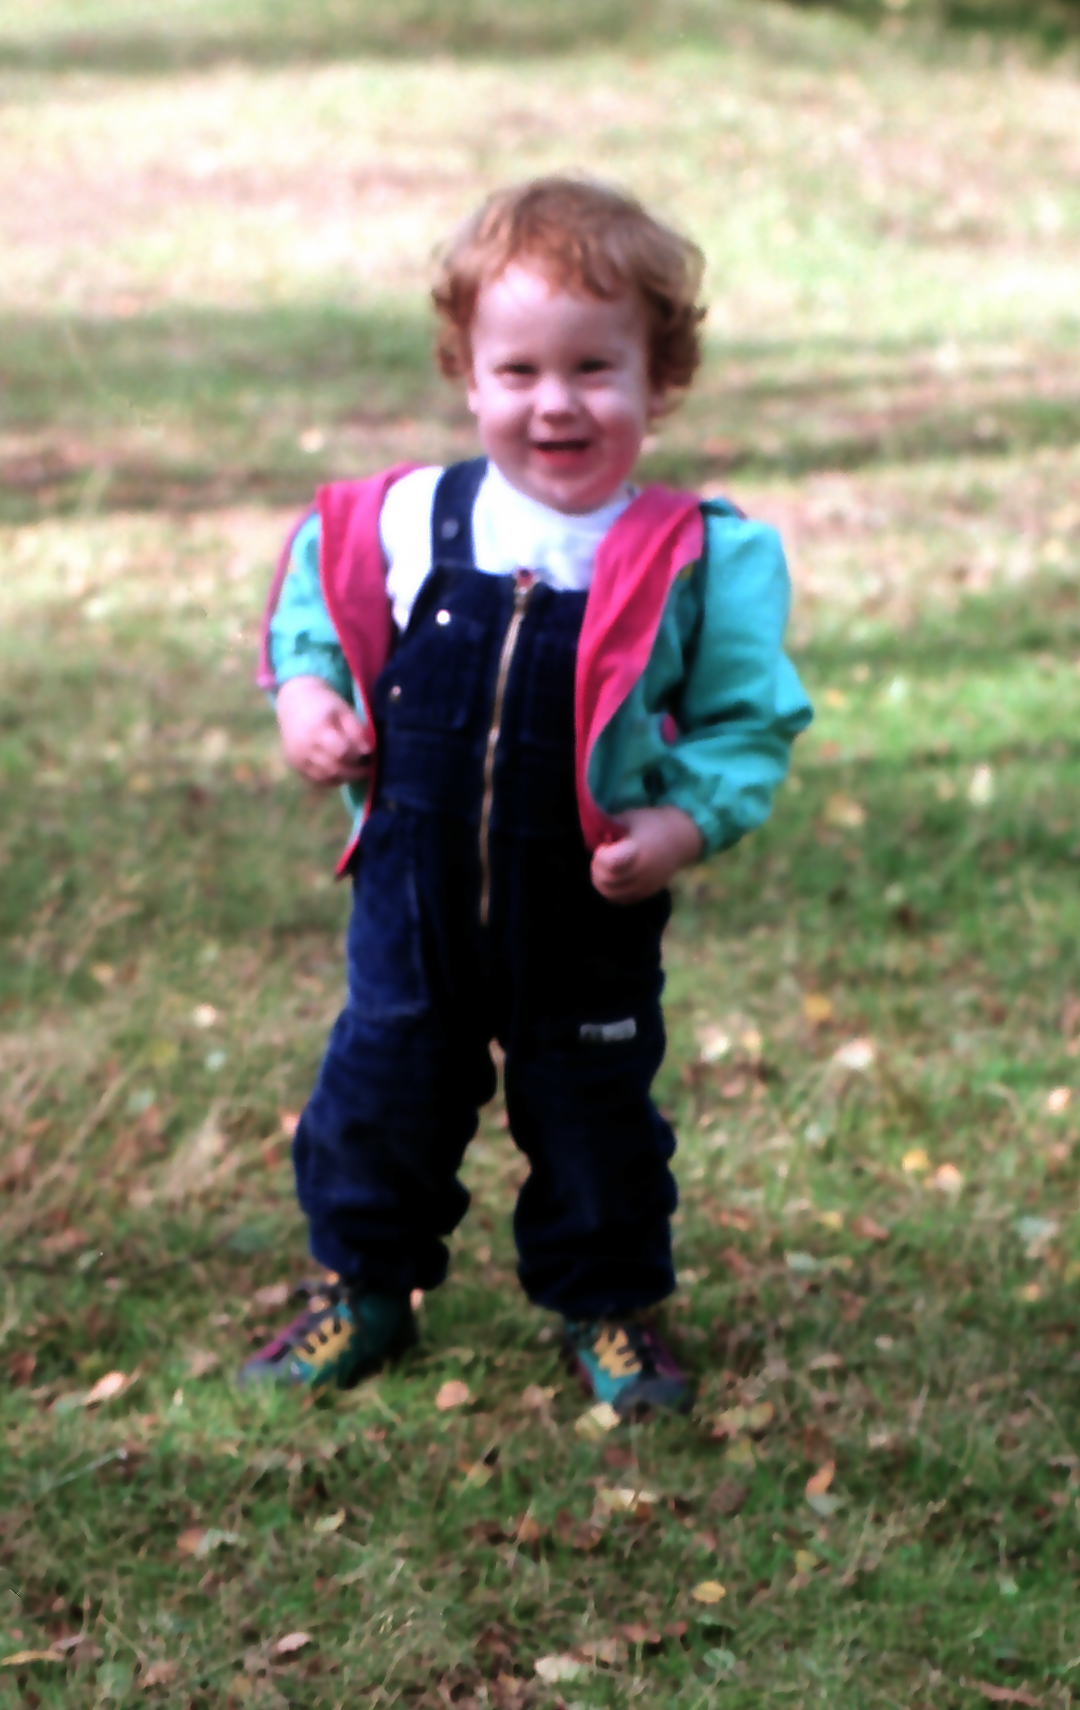
\includegraphics[width=1.0\textwidth]{images/0104.jpg}
        %\\
        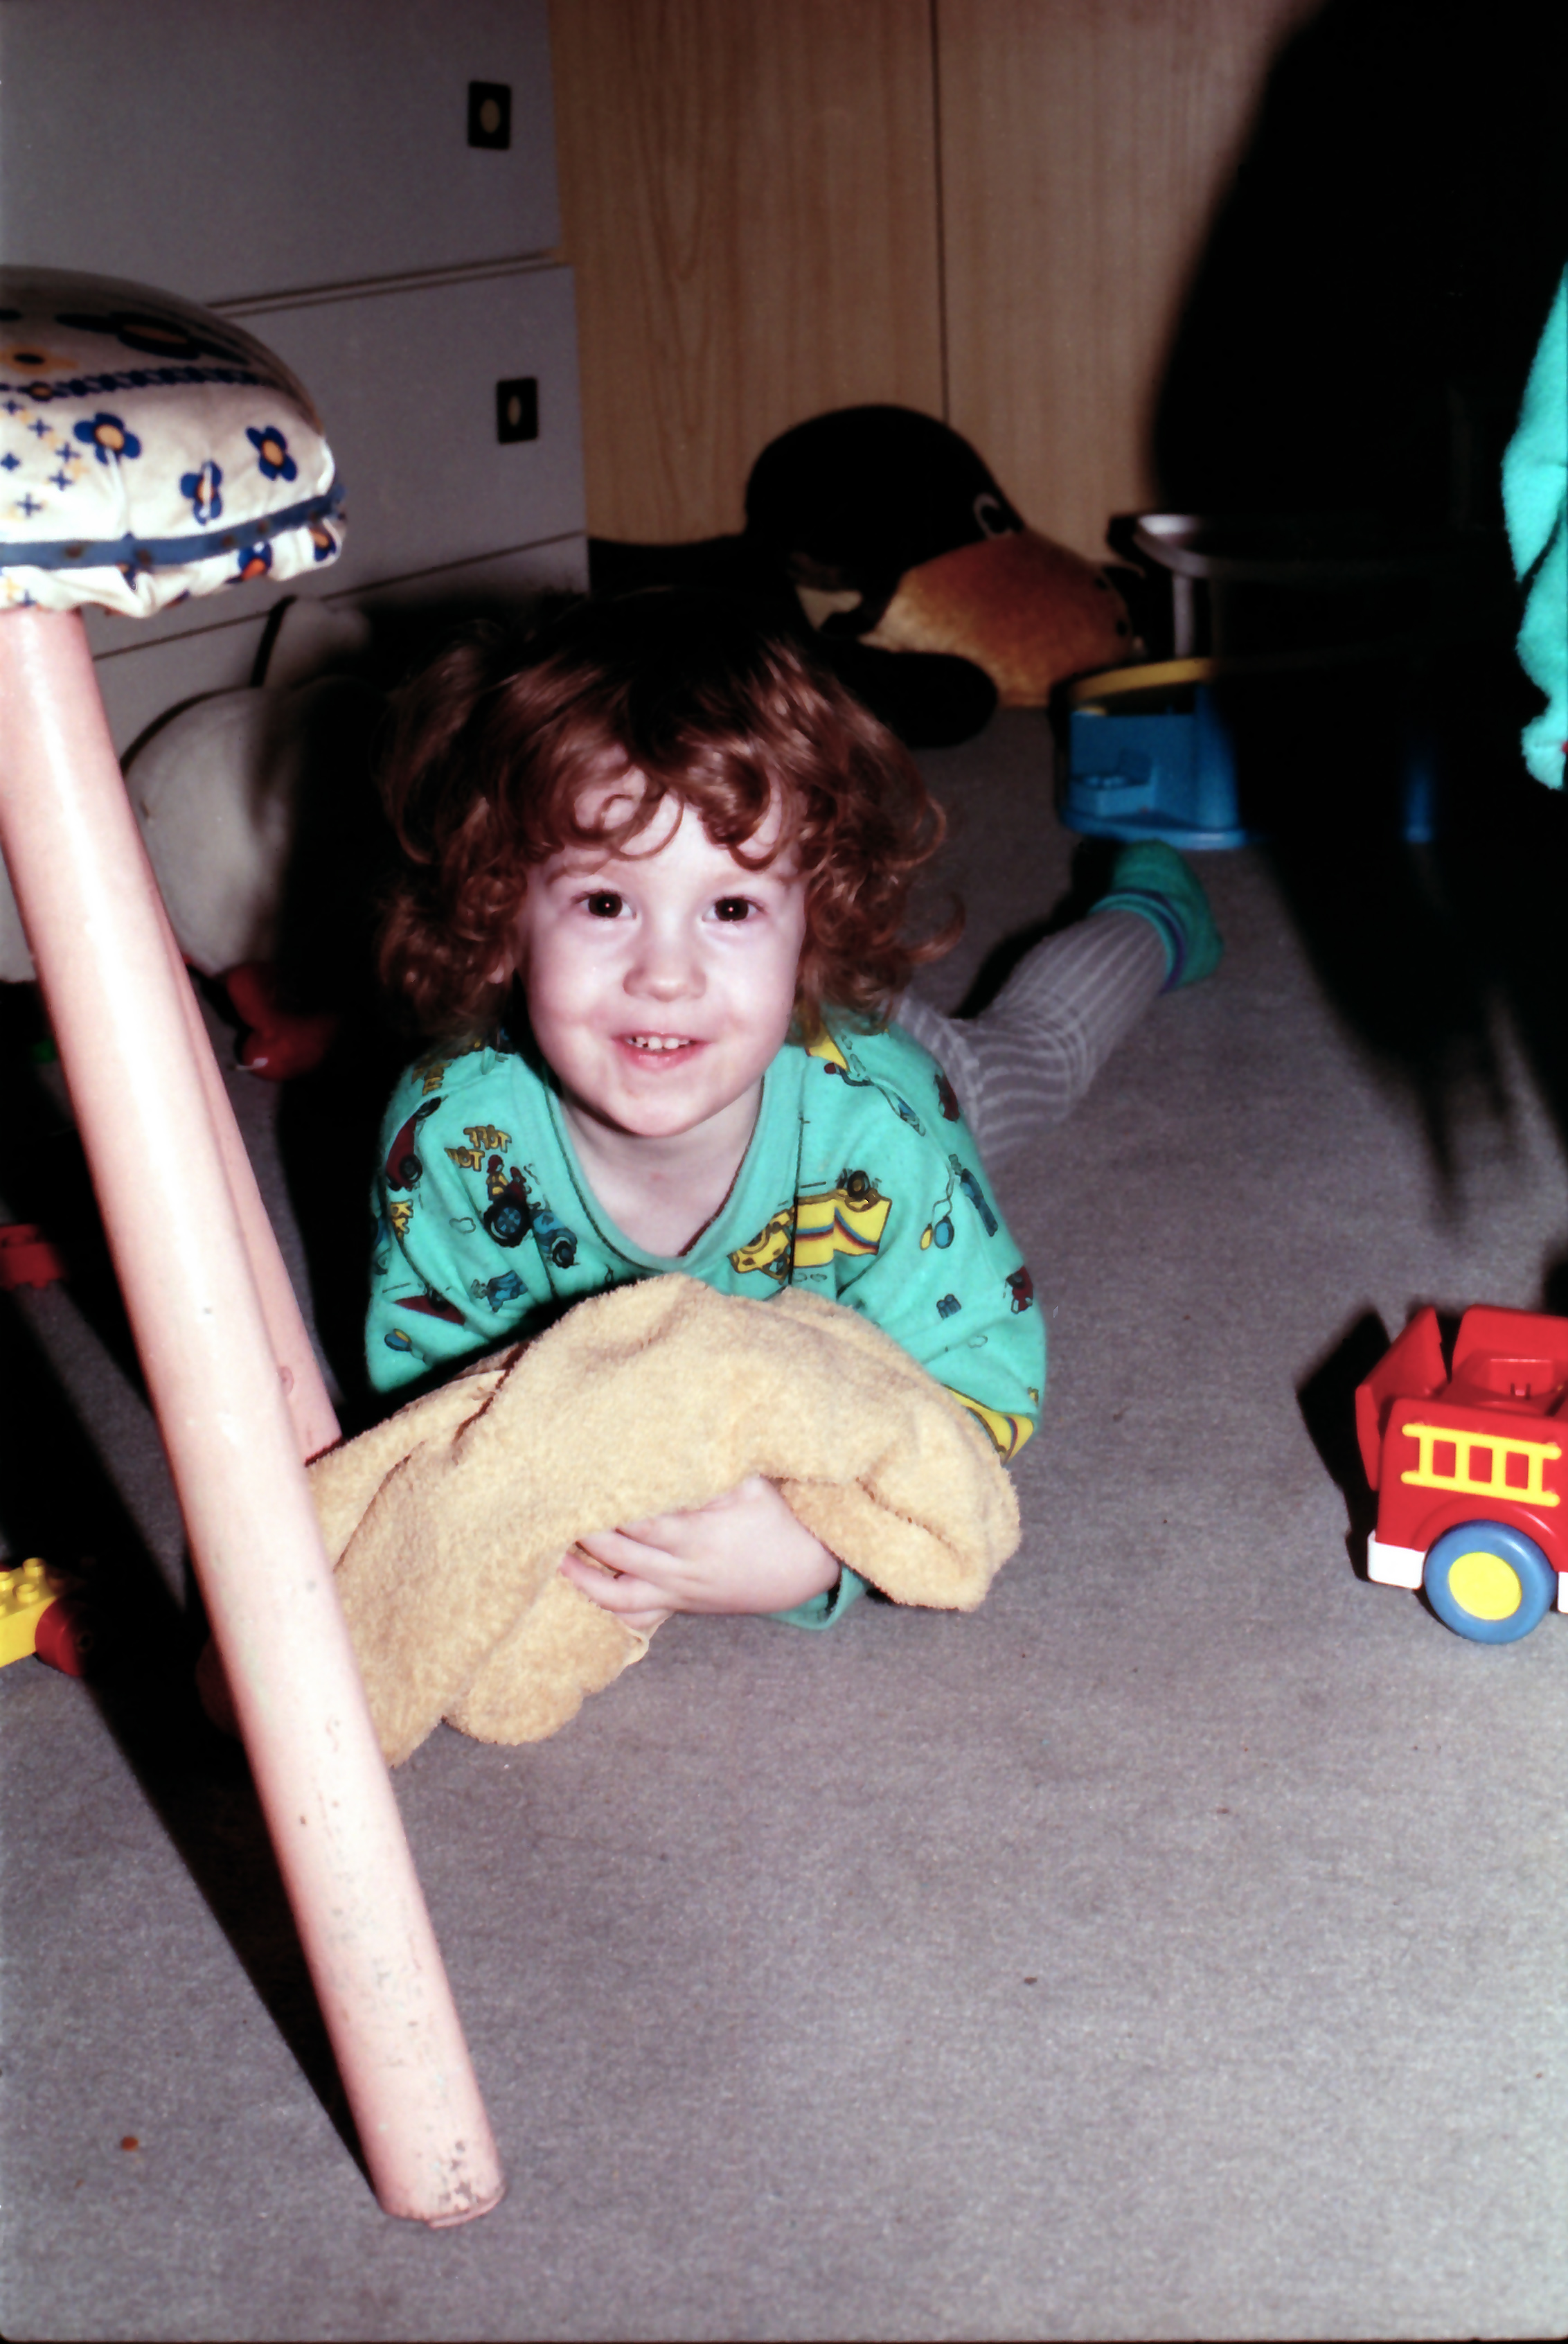
\includegraphics[width=1.0\textwidth]{images/0200.jpg}
    \end{minipage}%
    \begin{minipage}{.65\textwidth}
        \centering
        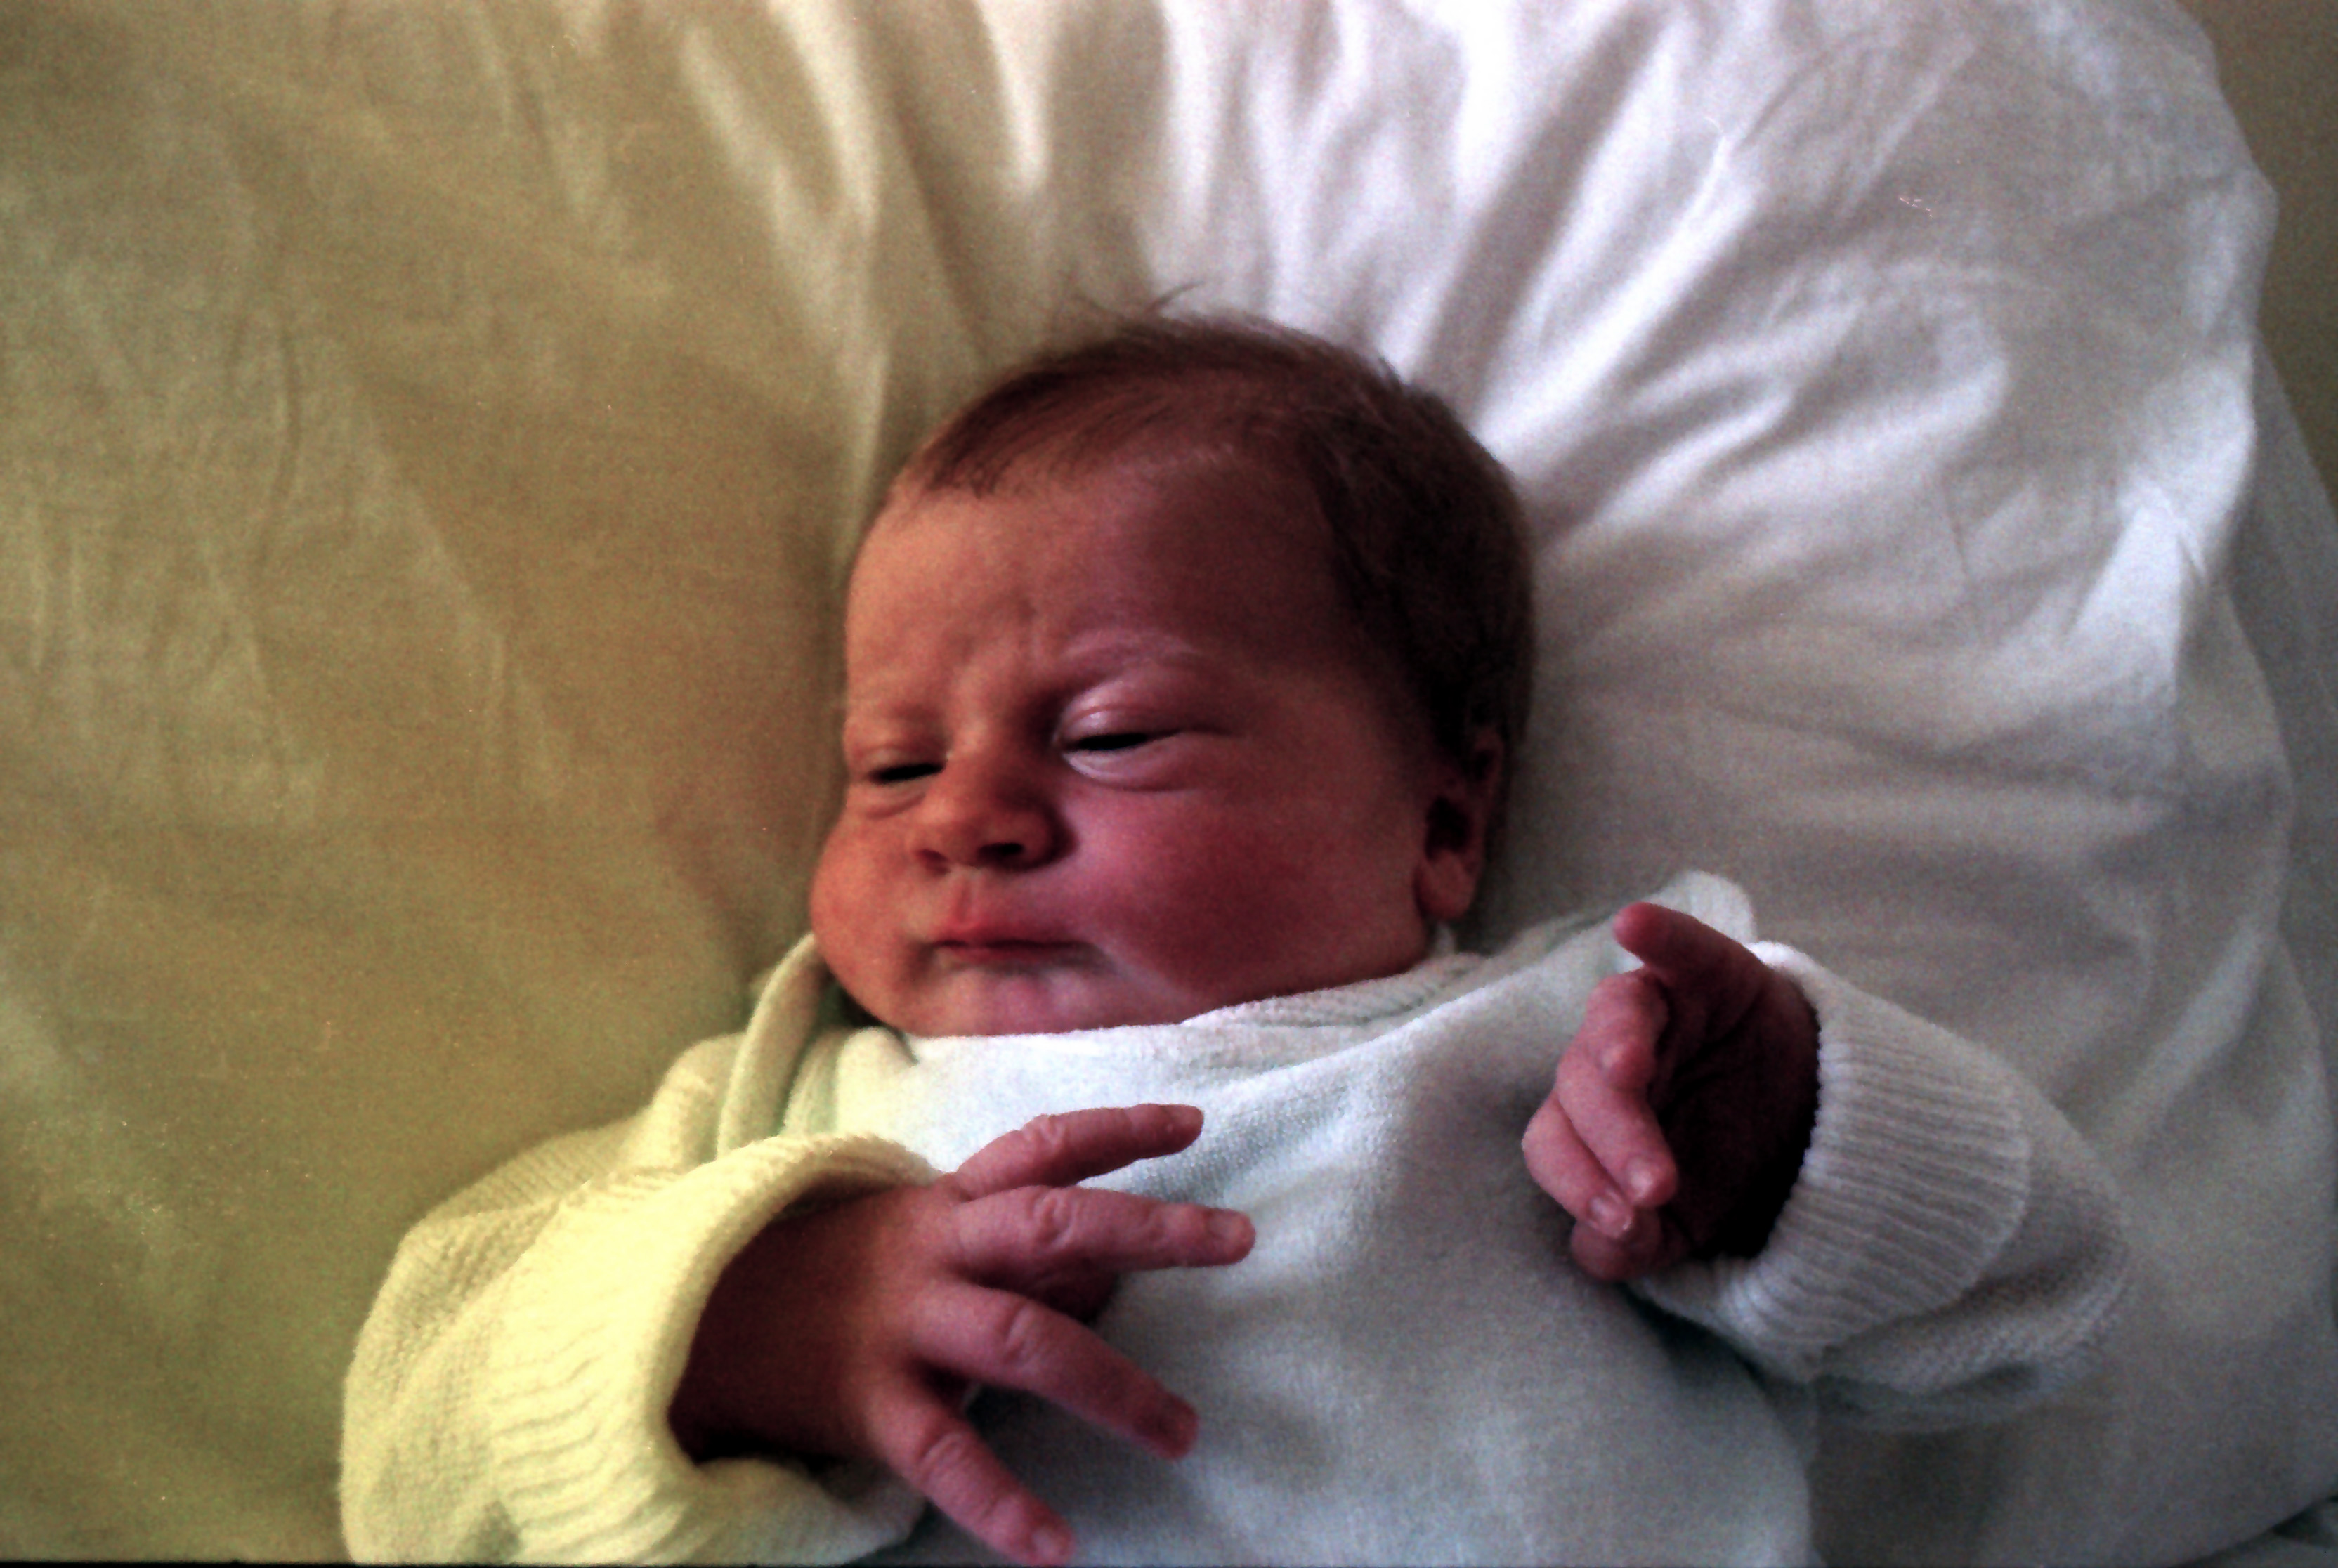
\includegraphics[width=.33\textwidth]{images/0101.jpg}%
        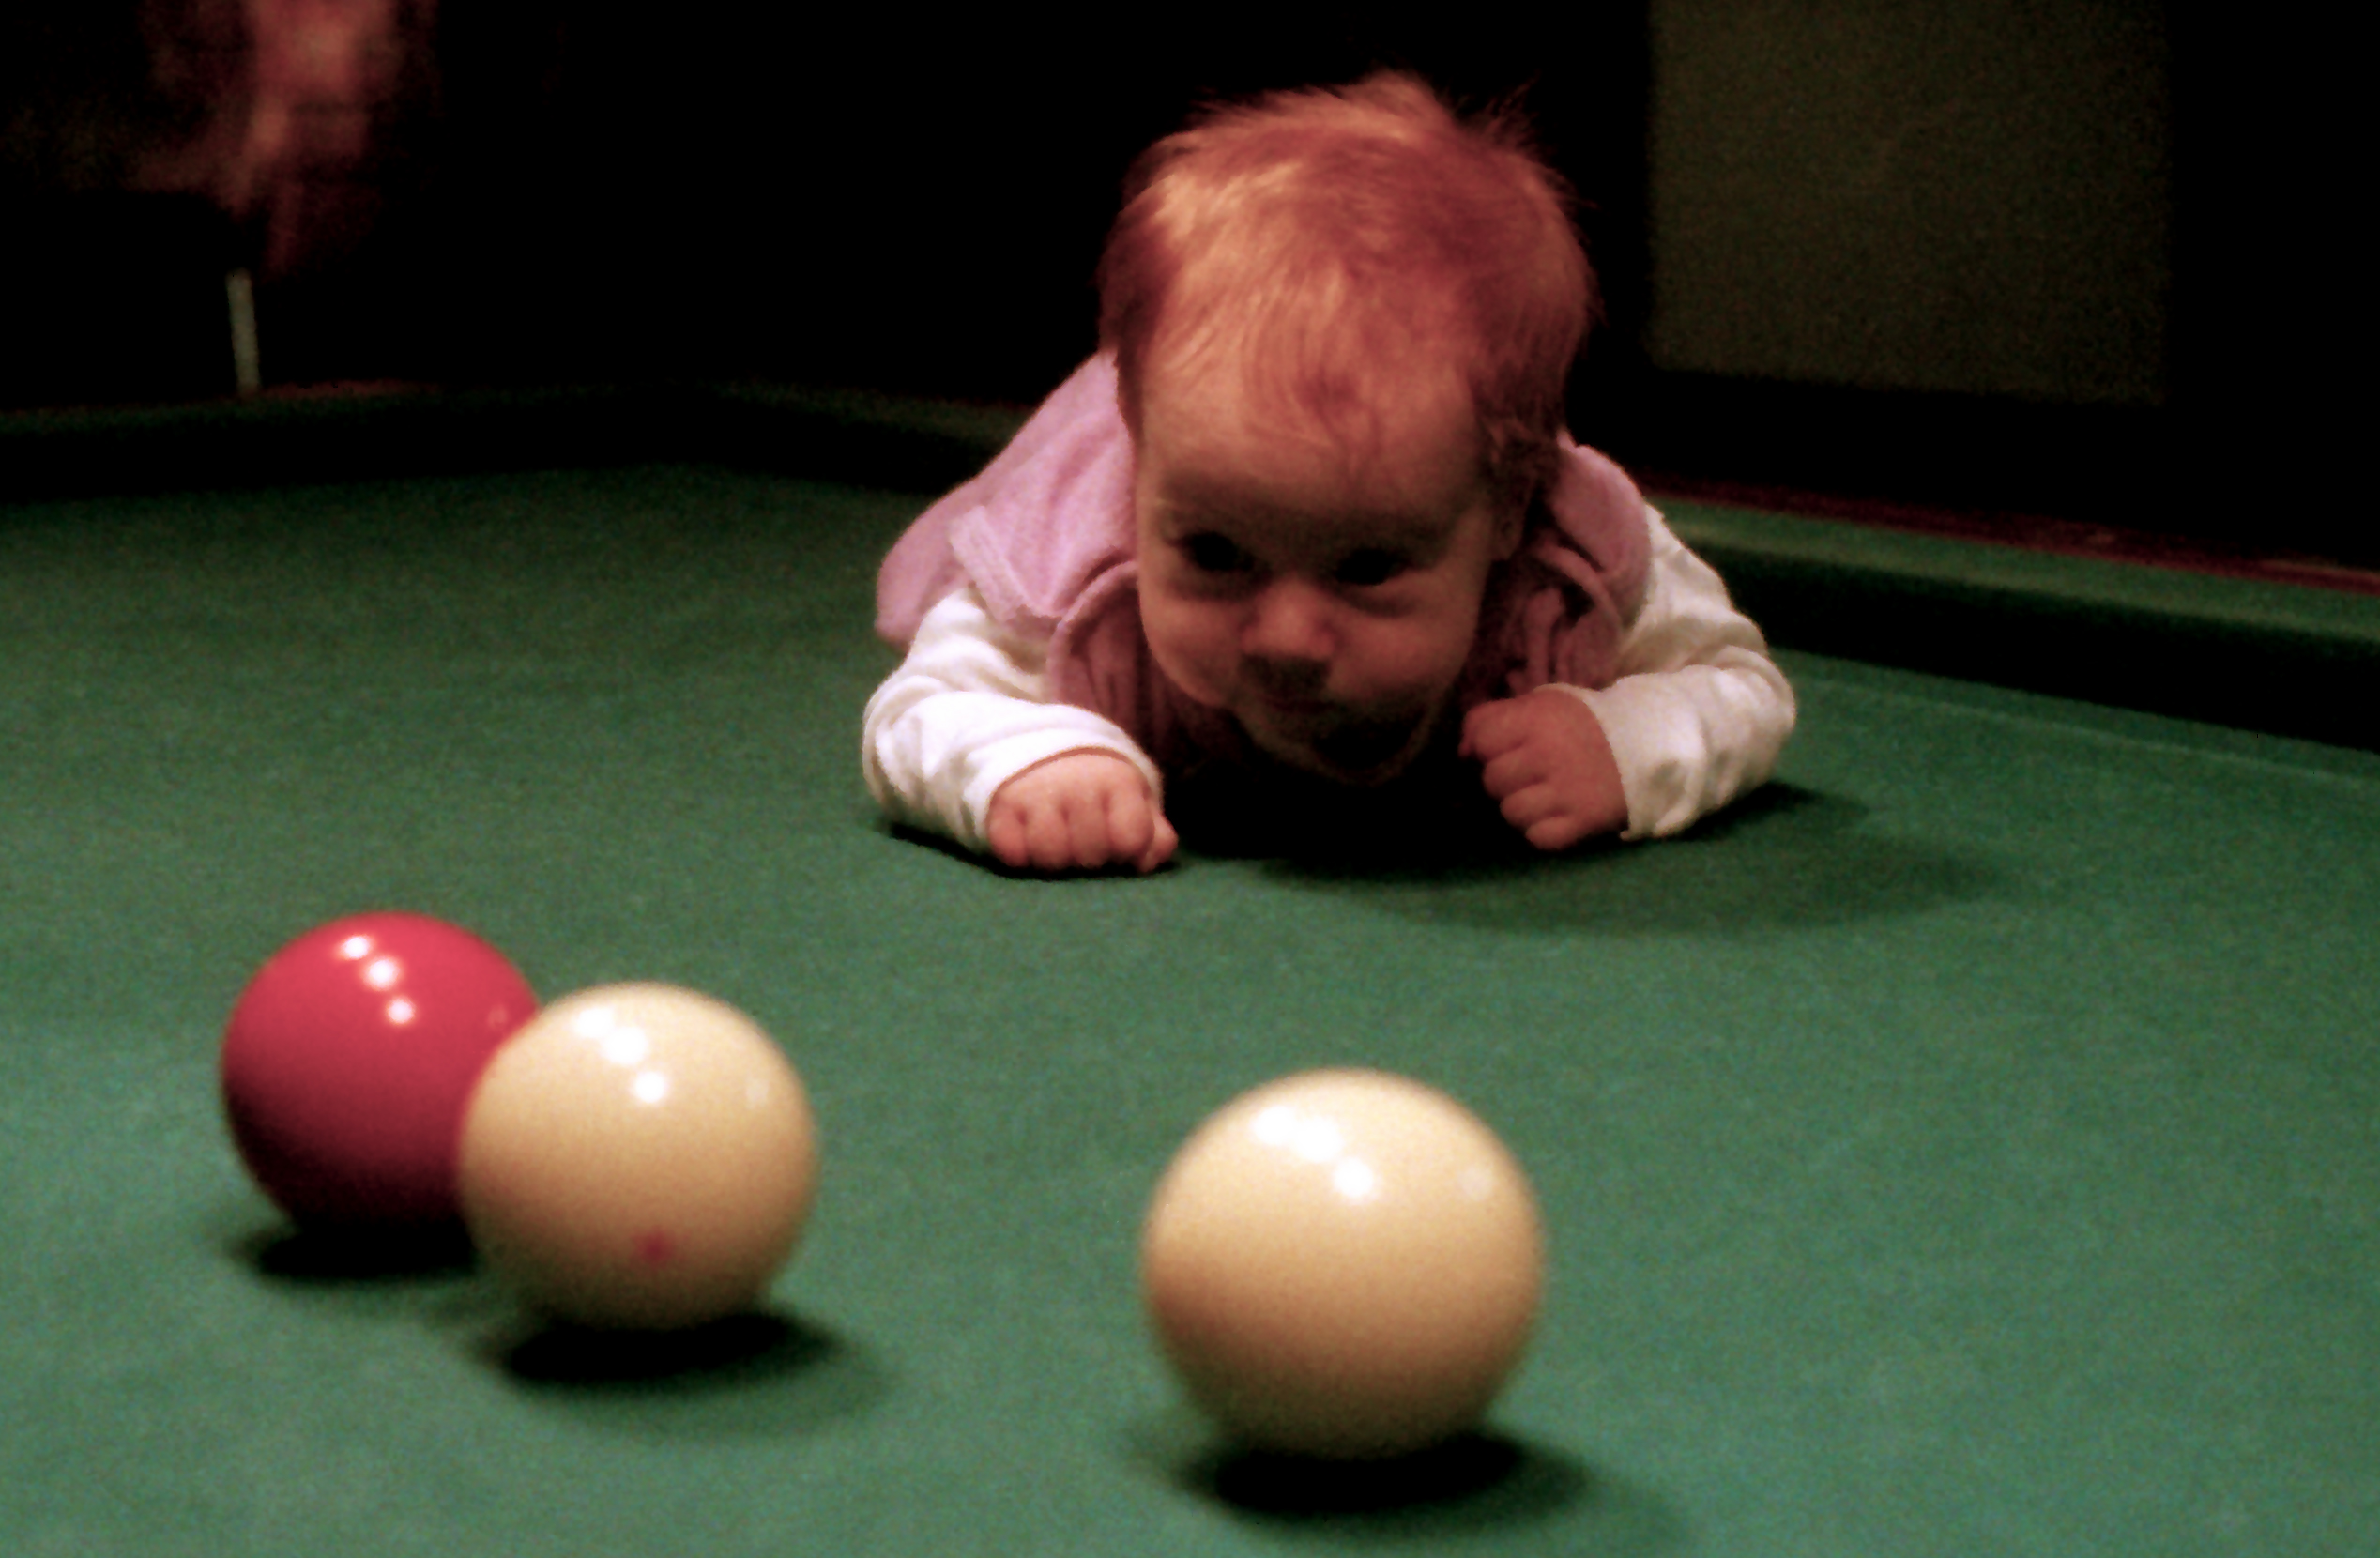
\includegraphics[width=.33\textwidth]{images/0102.jpg}%
        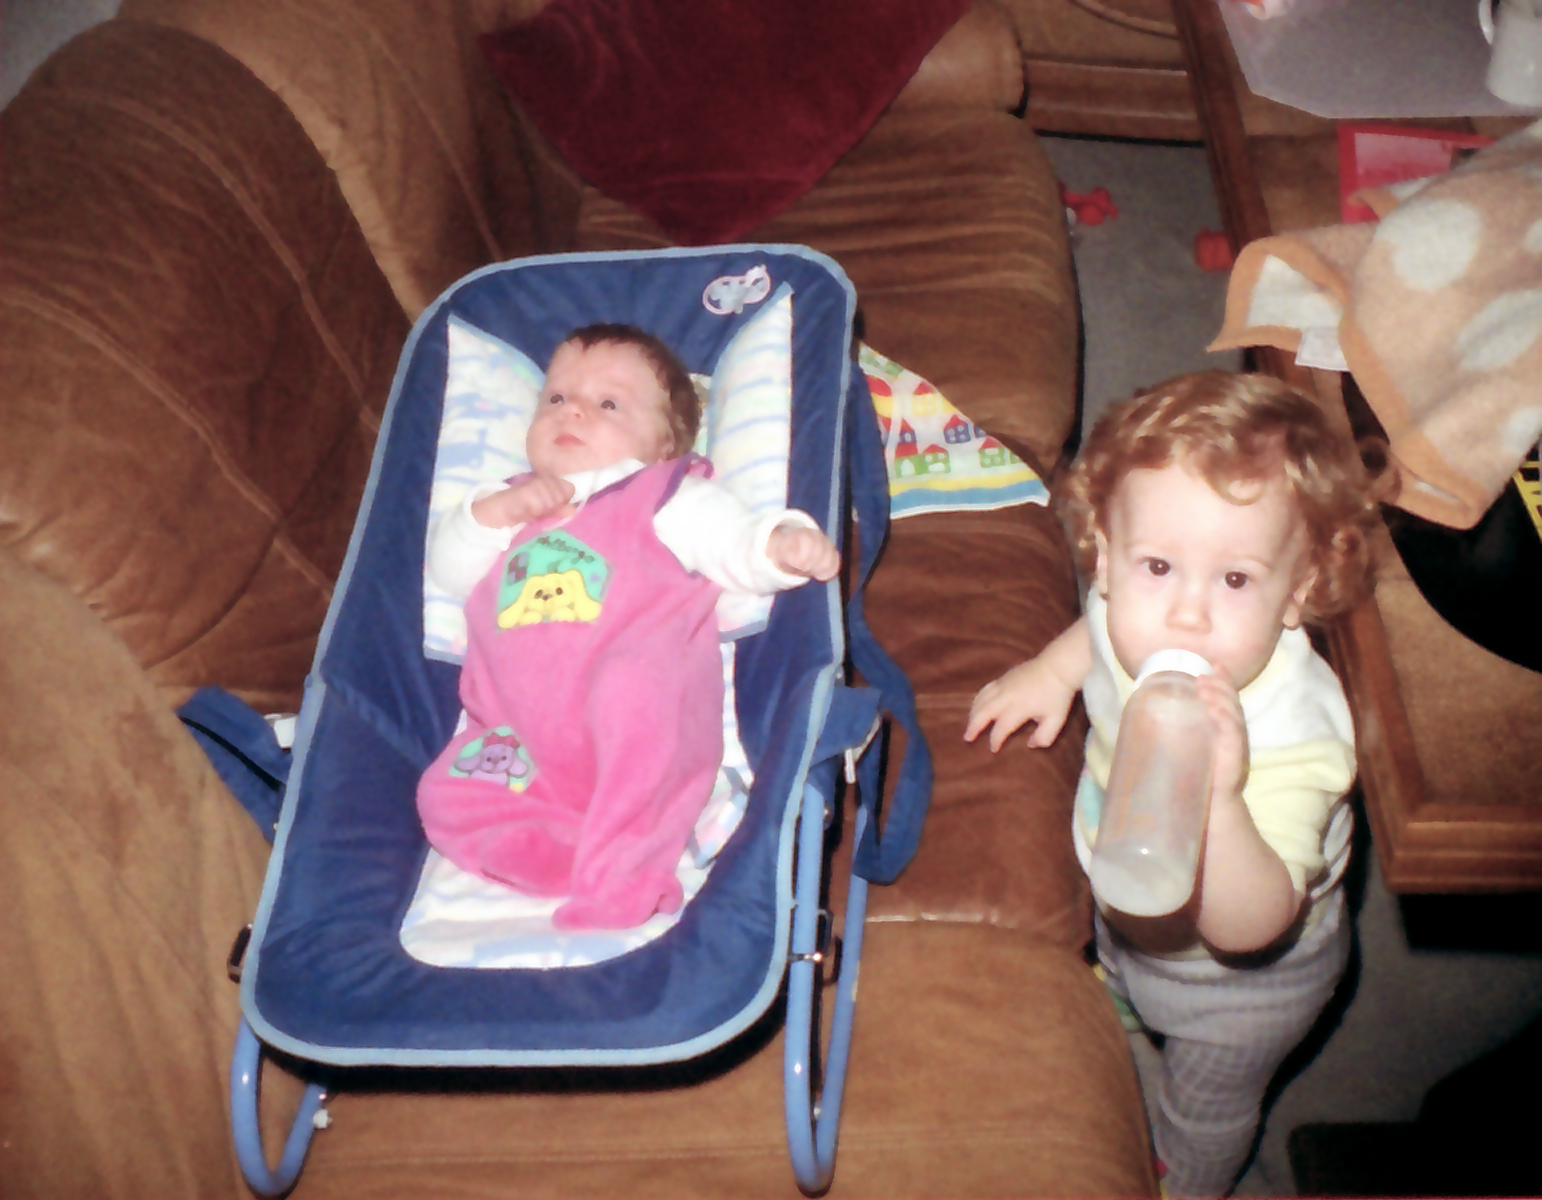
\includegraphics[width=.33\textwidth]{images/0103.jpg}
        %\\
        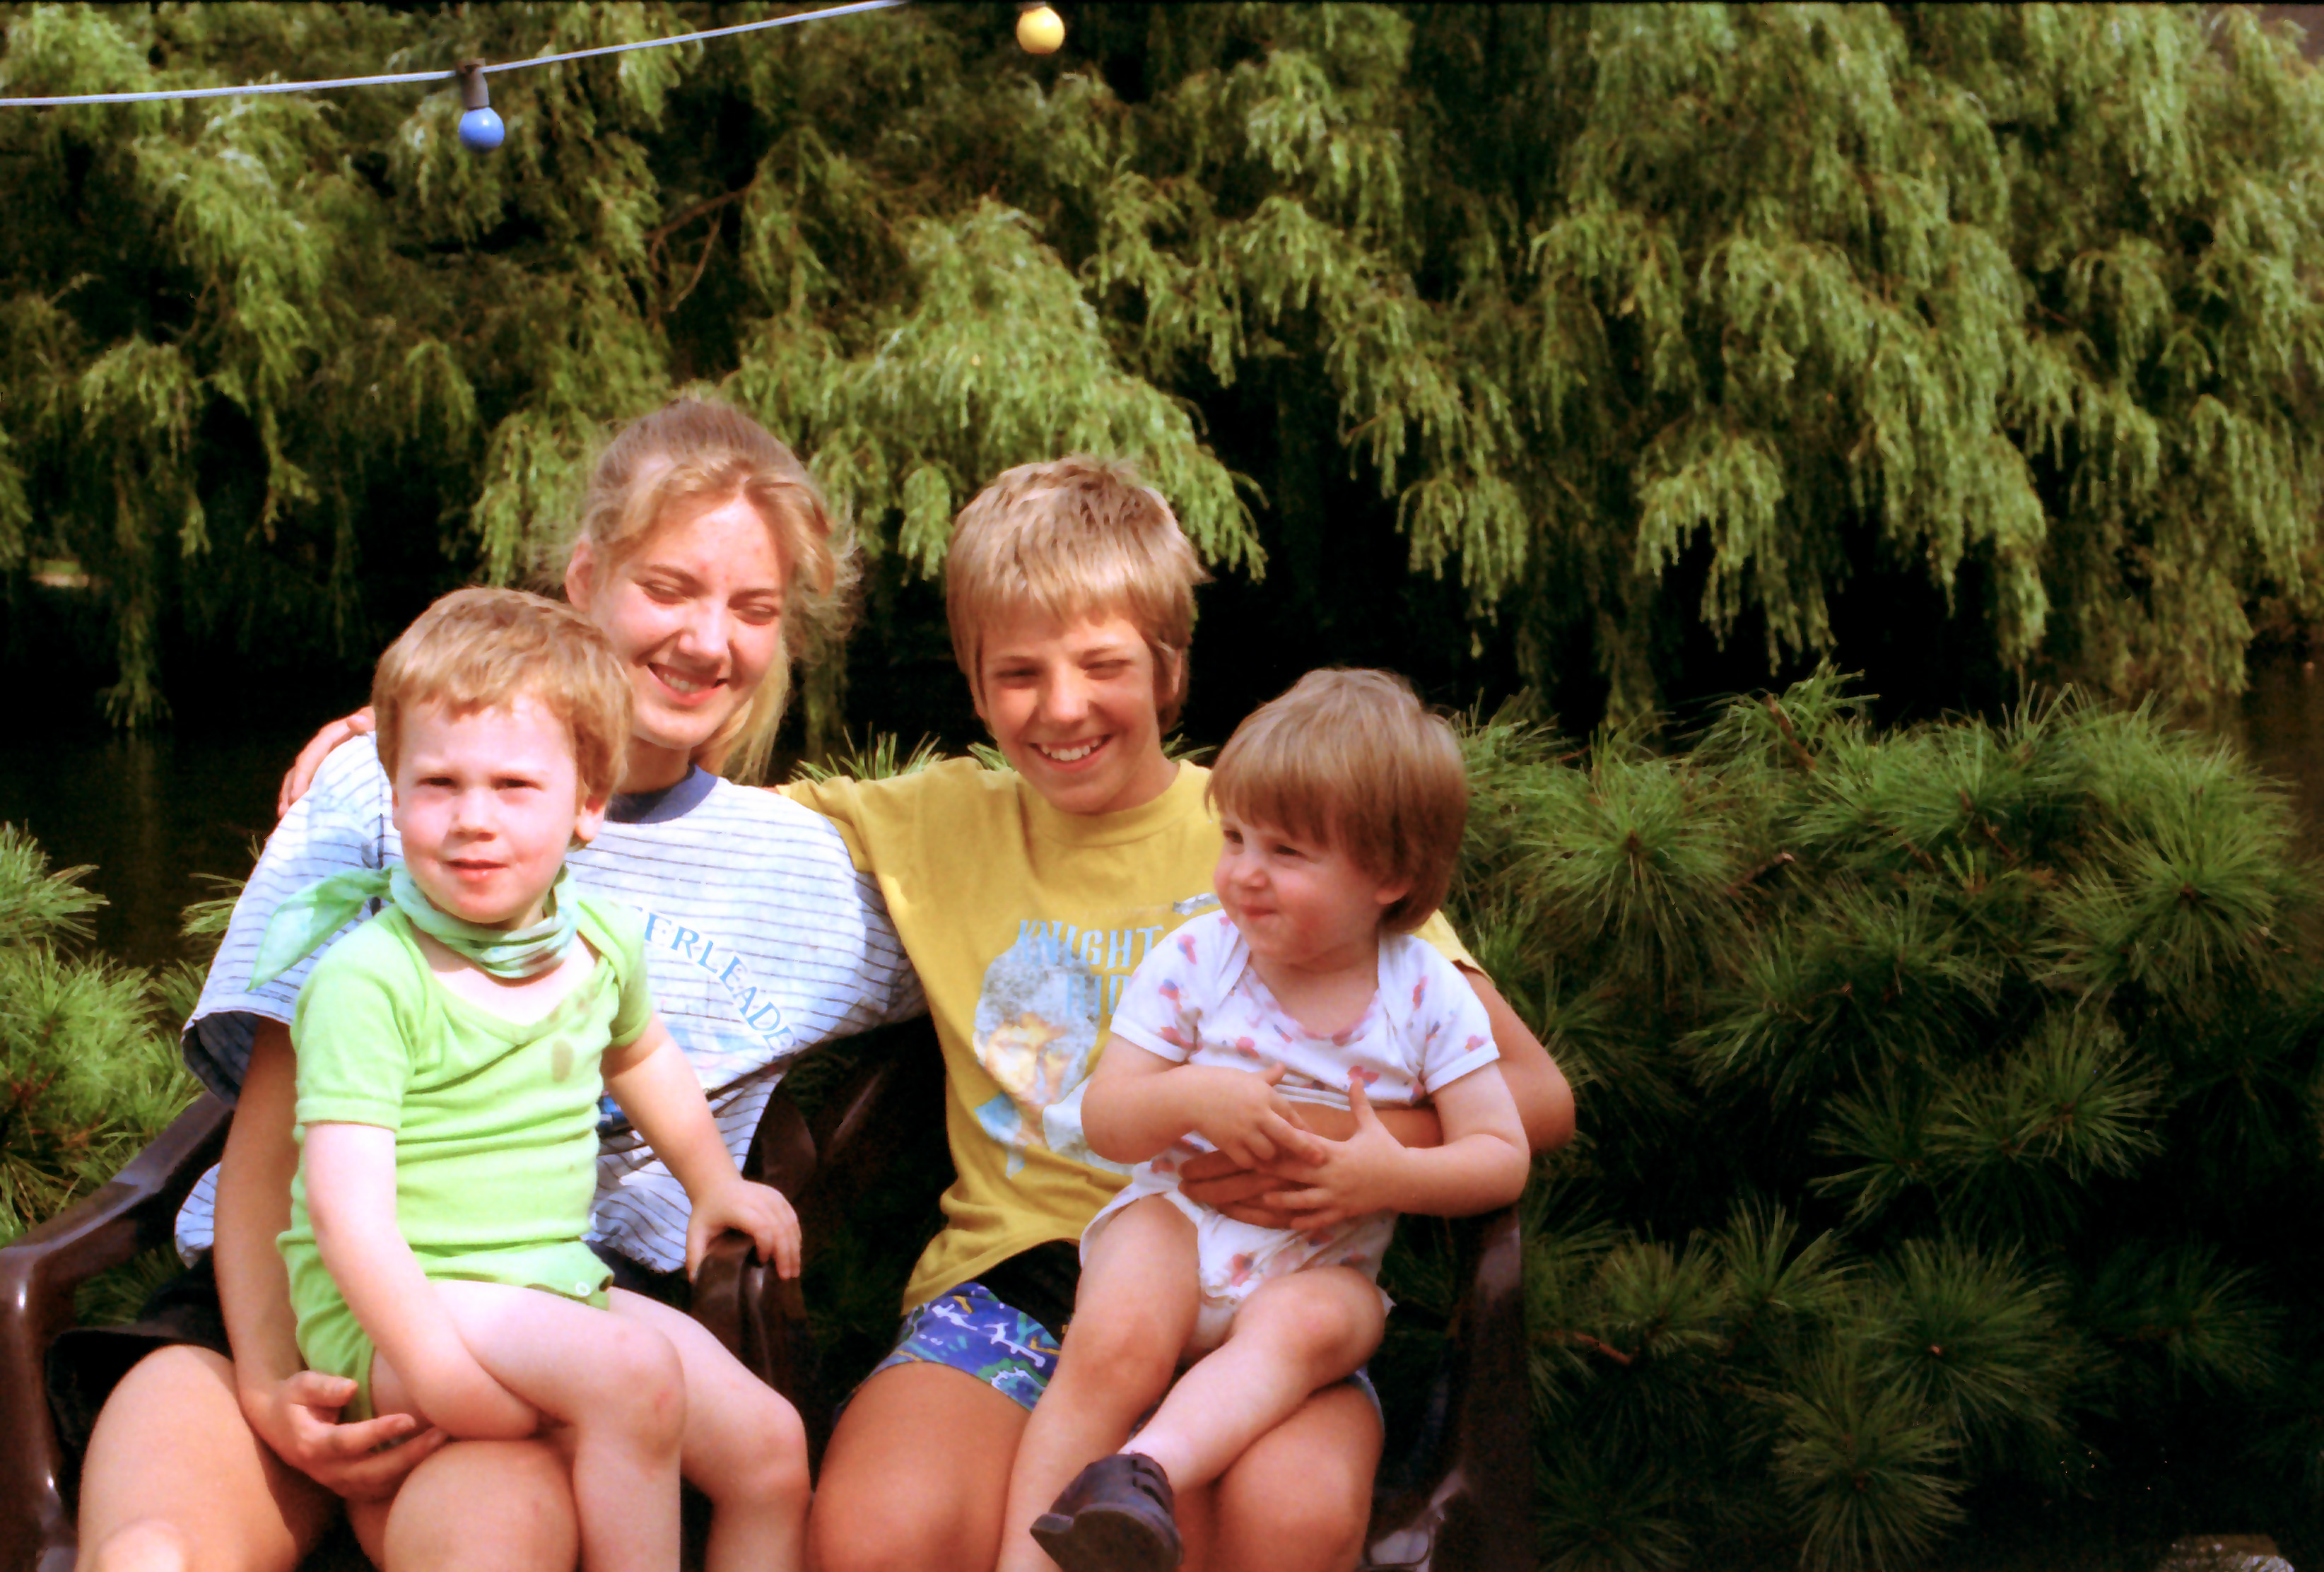
\includegraphics[width=.33\textwidth]{images/0201.jpg}%
        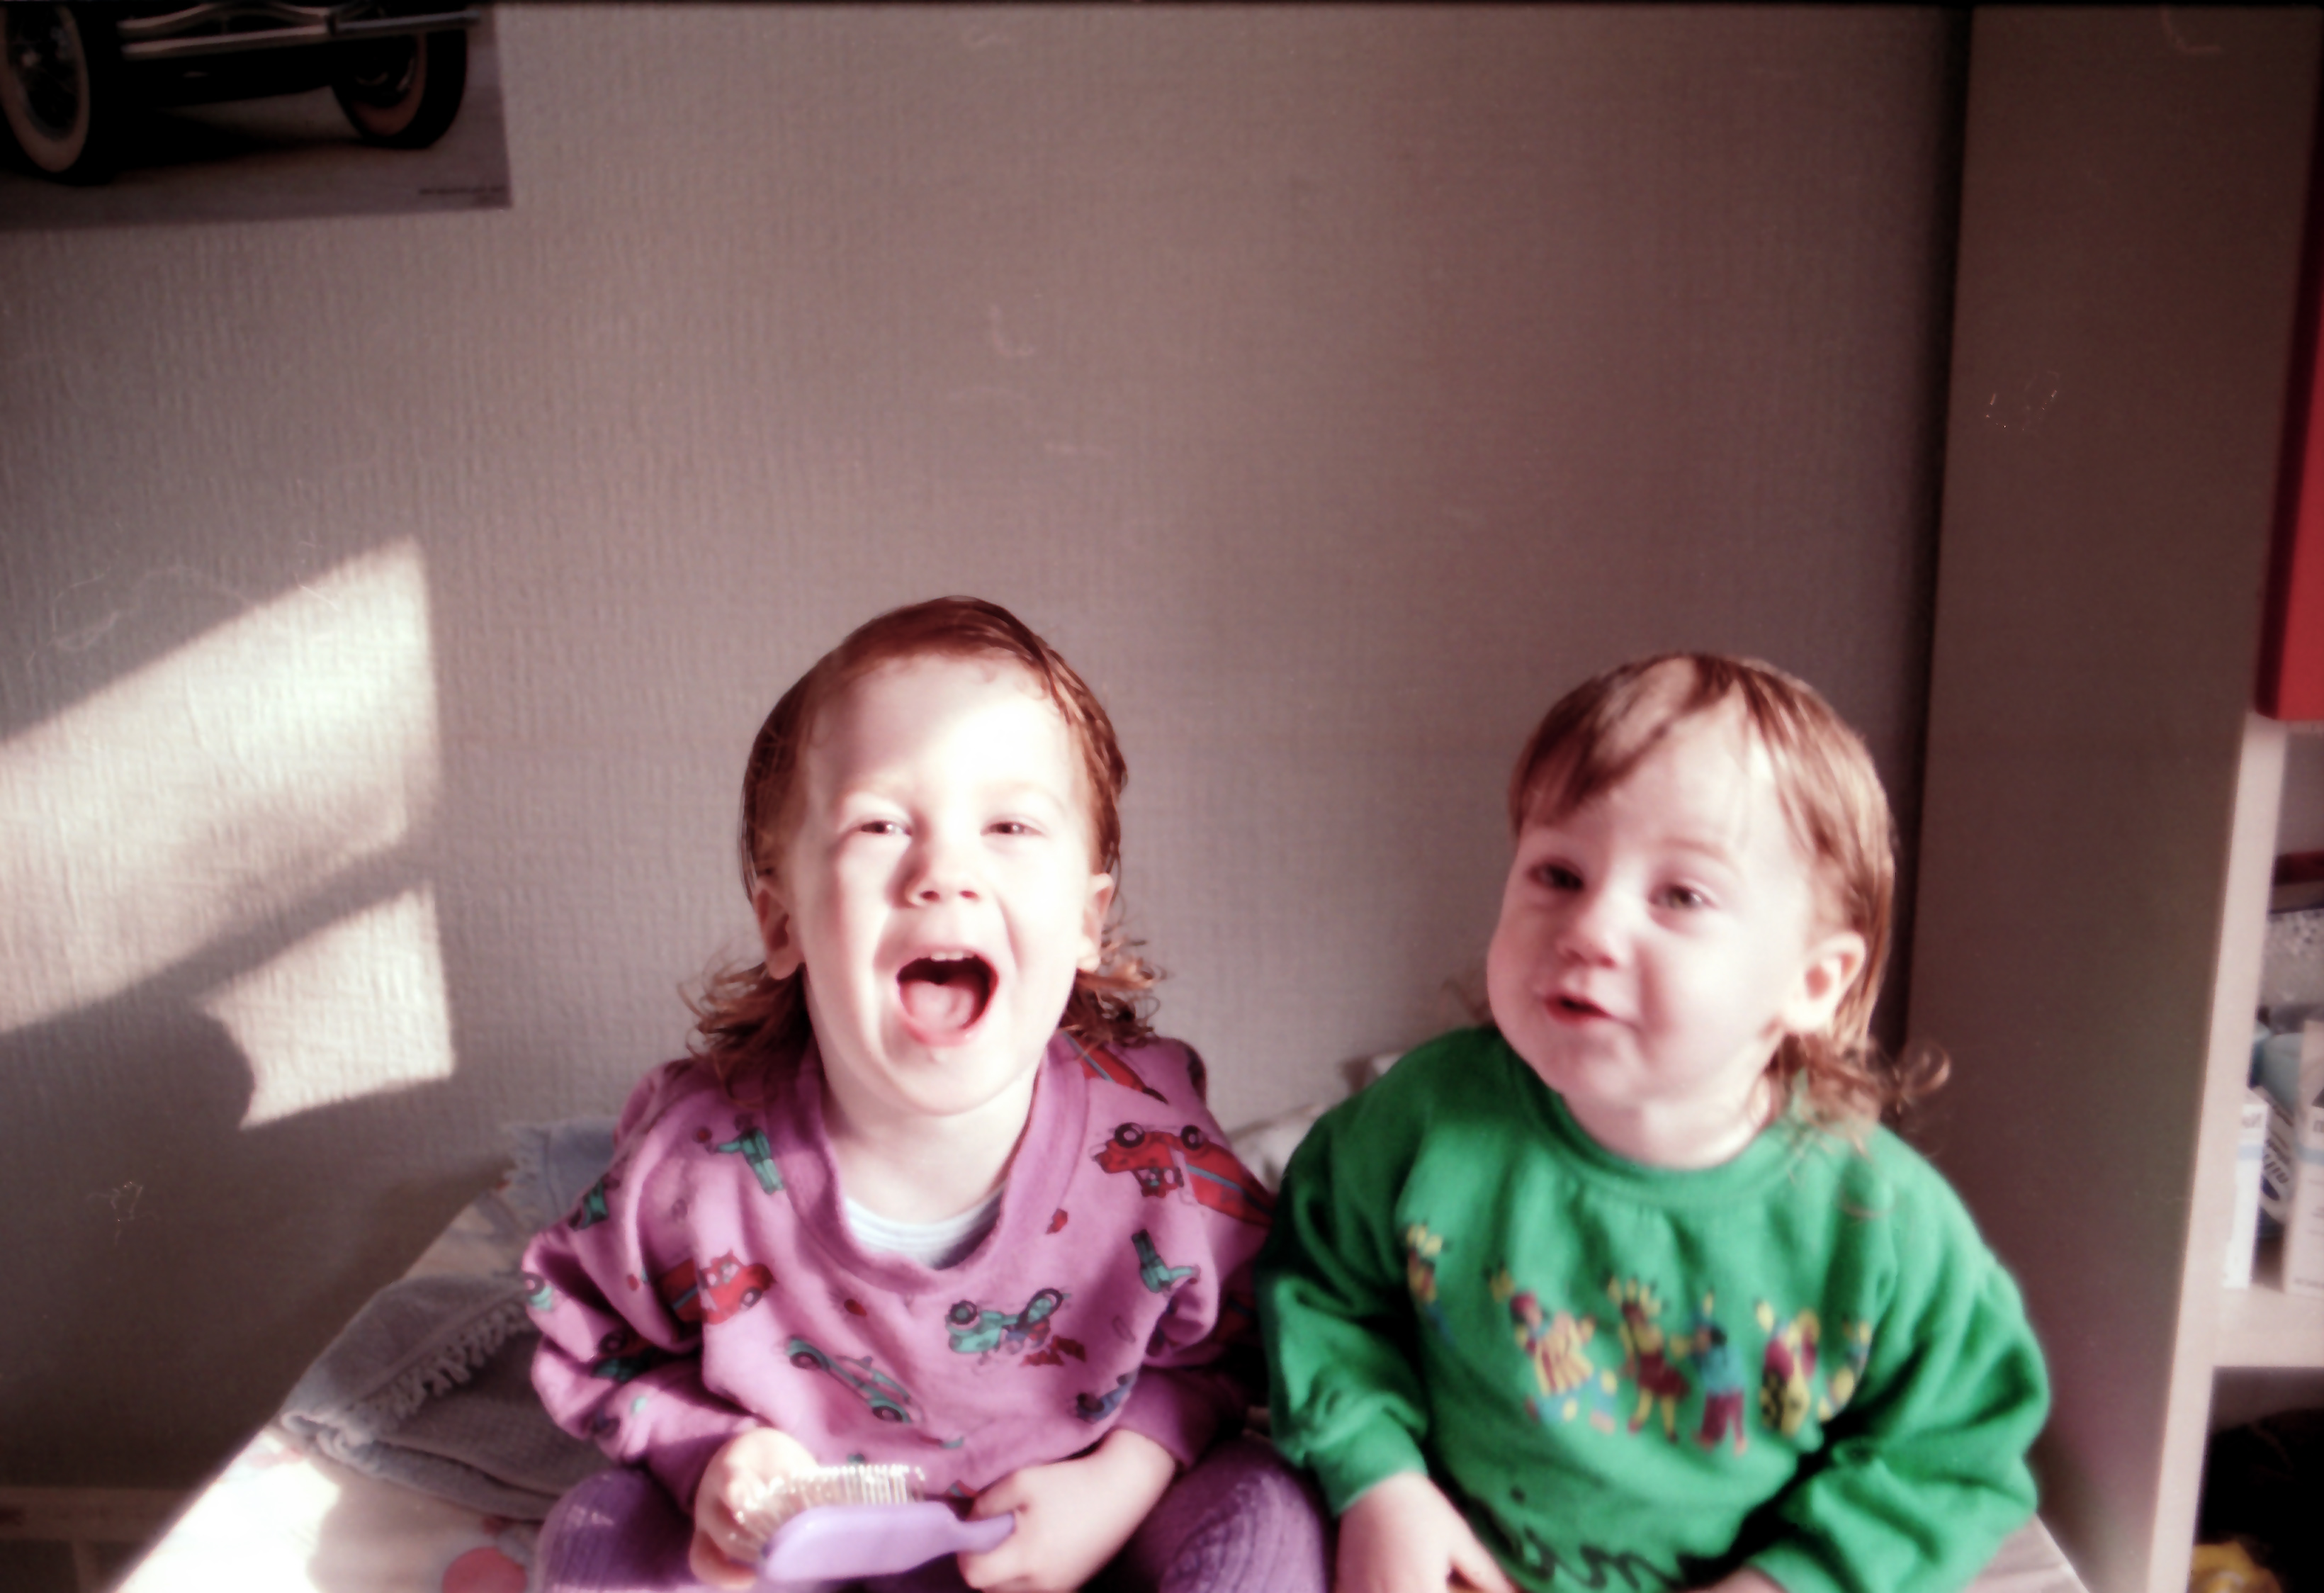
\includegraphics[width=.33\textwidth]{images/0202.jpg}%
        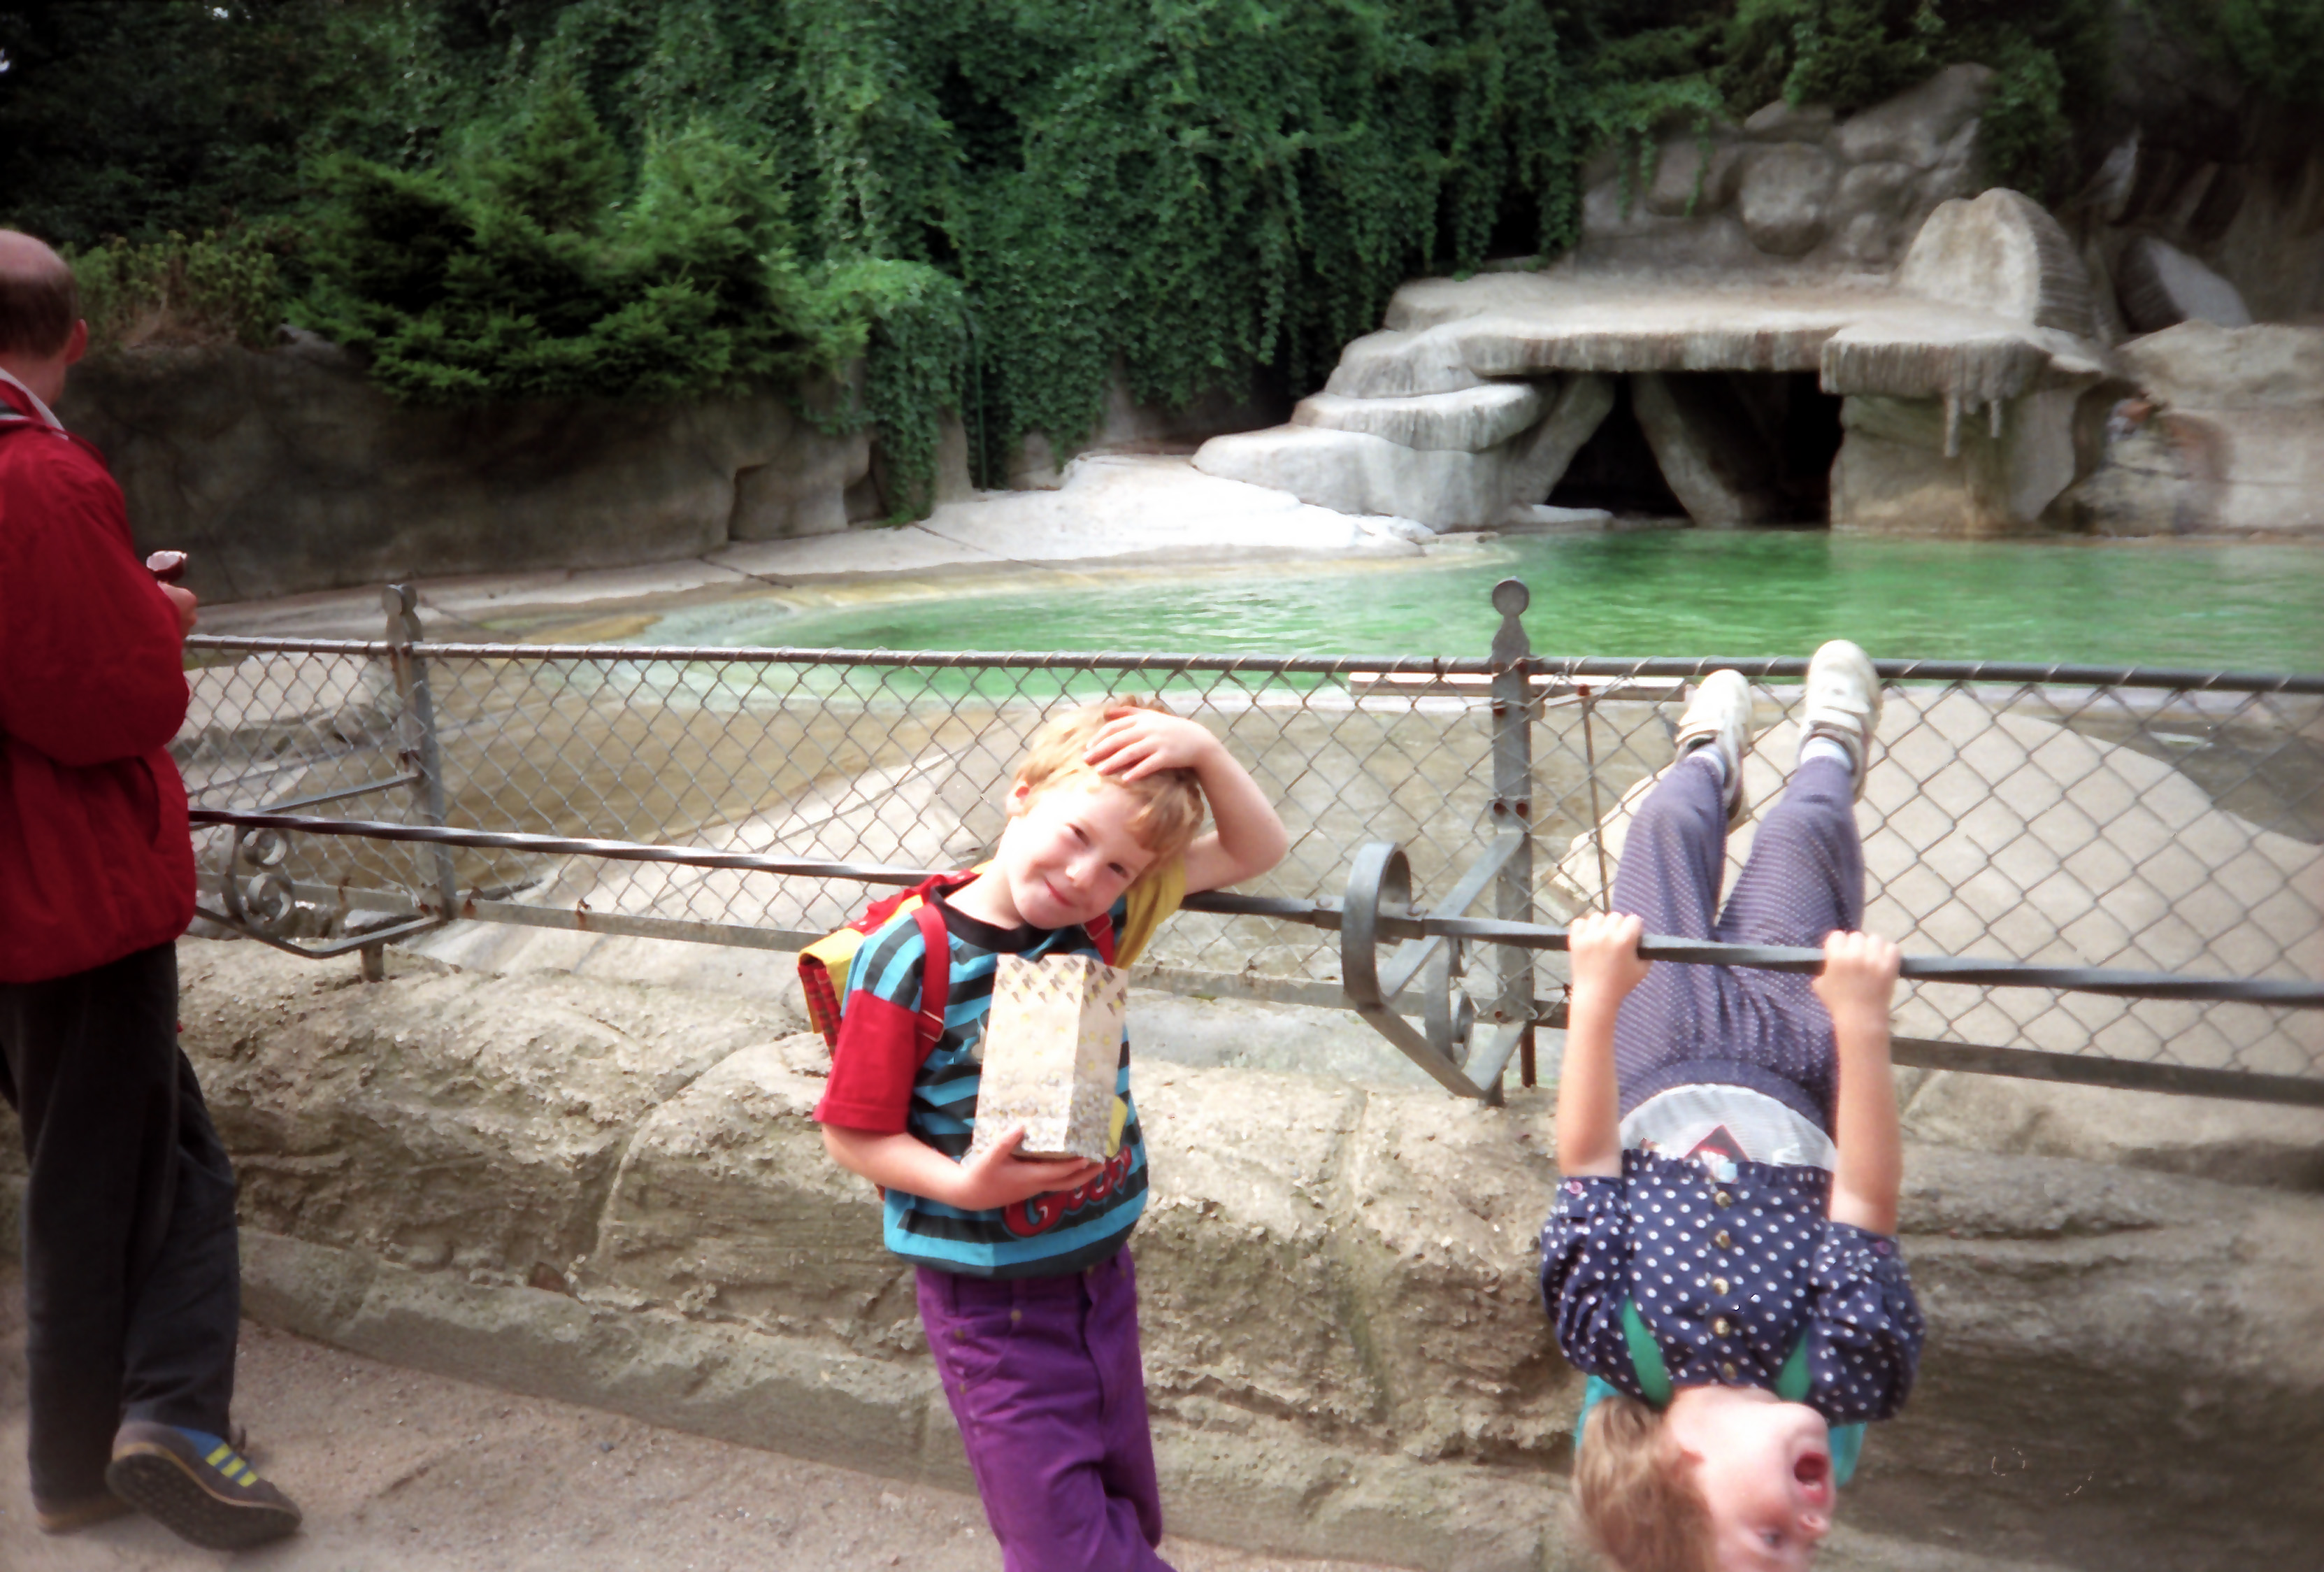
\includegraphics[width=.33\textwidth]{images/0203.jpg}
        %\\
        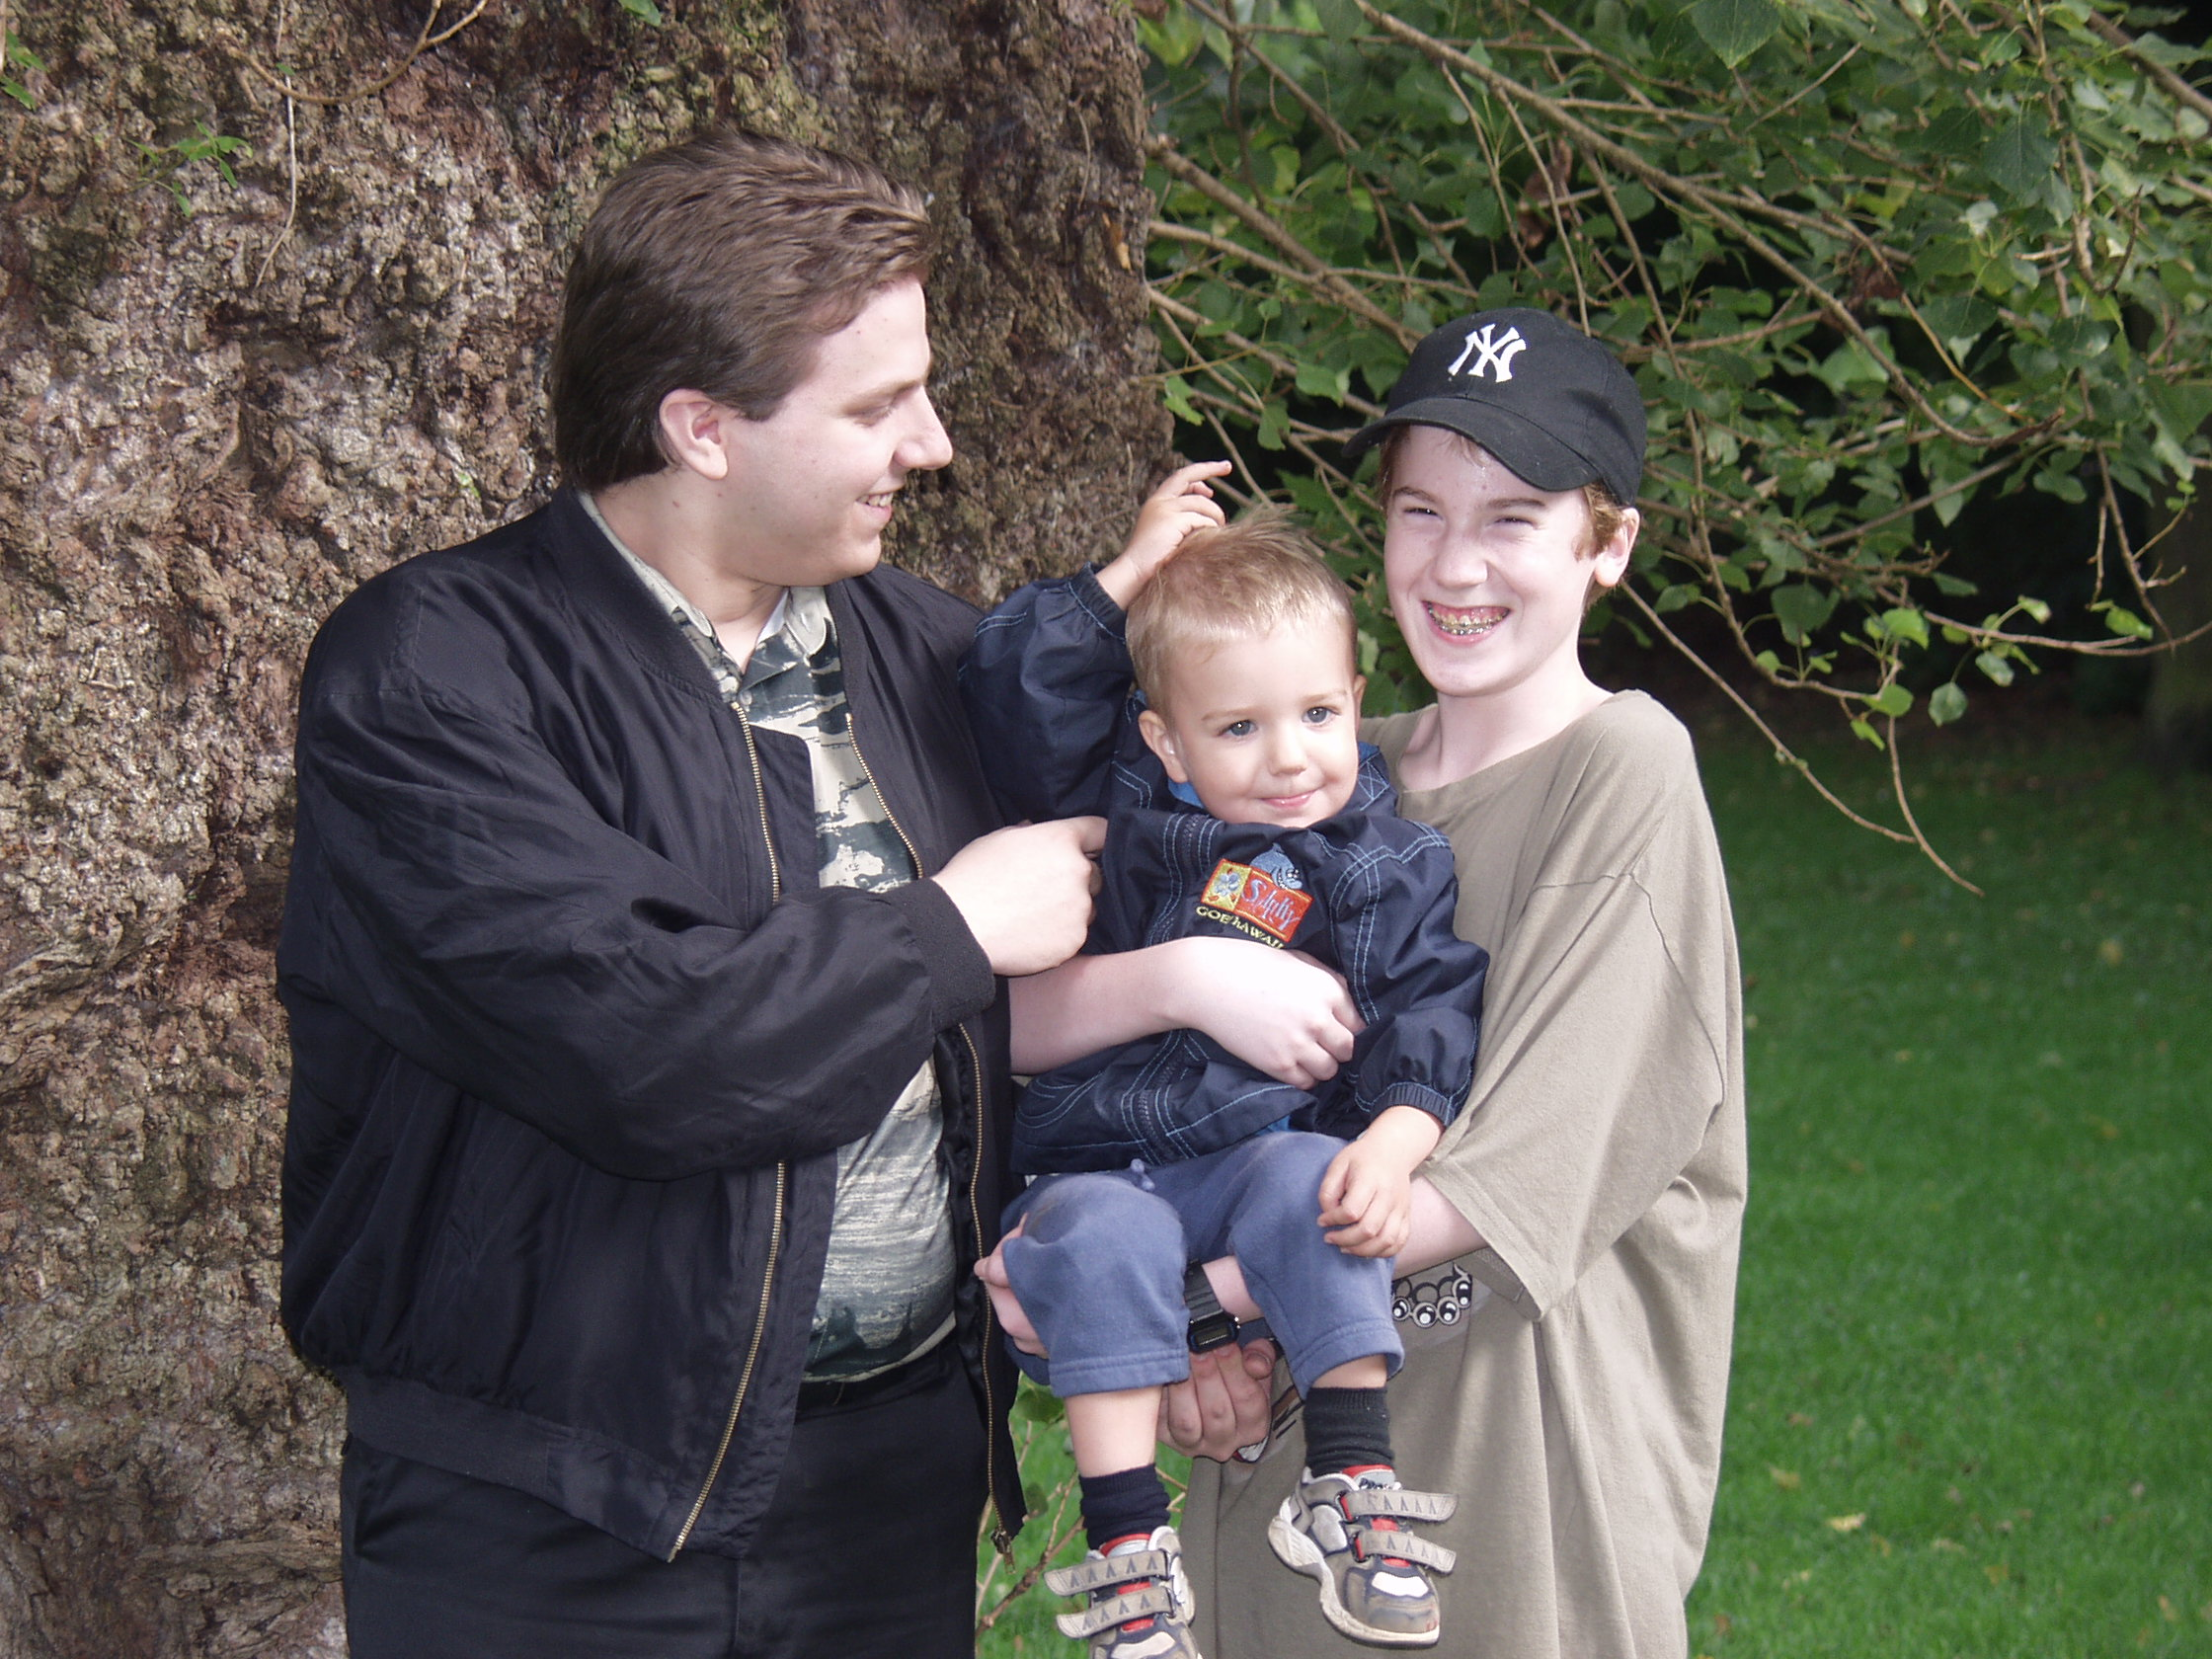
\includegraphics[width=.33\textwidth]{images/0301.jpg}%
        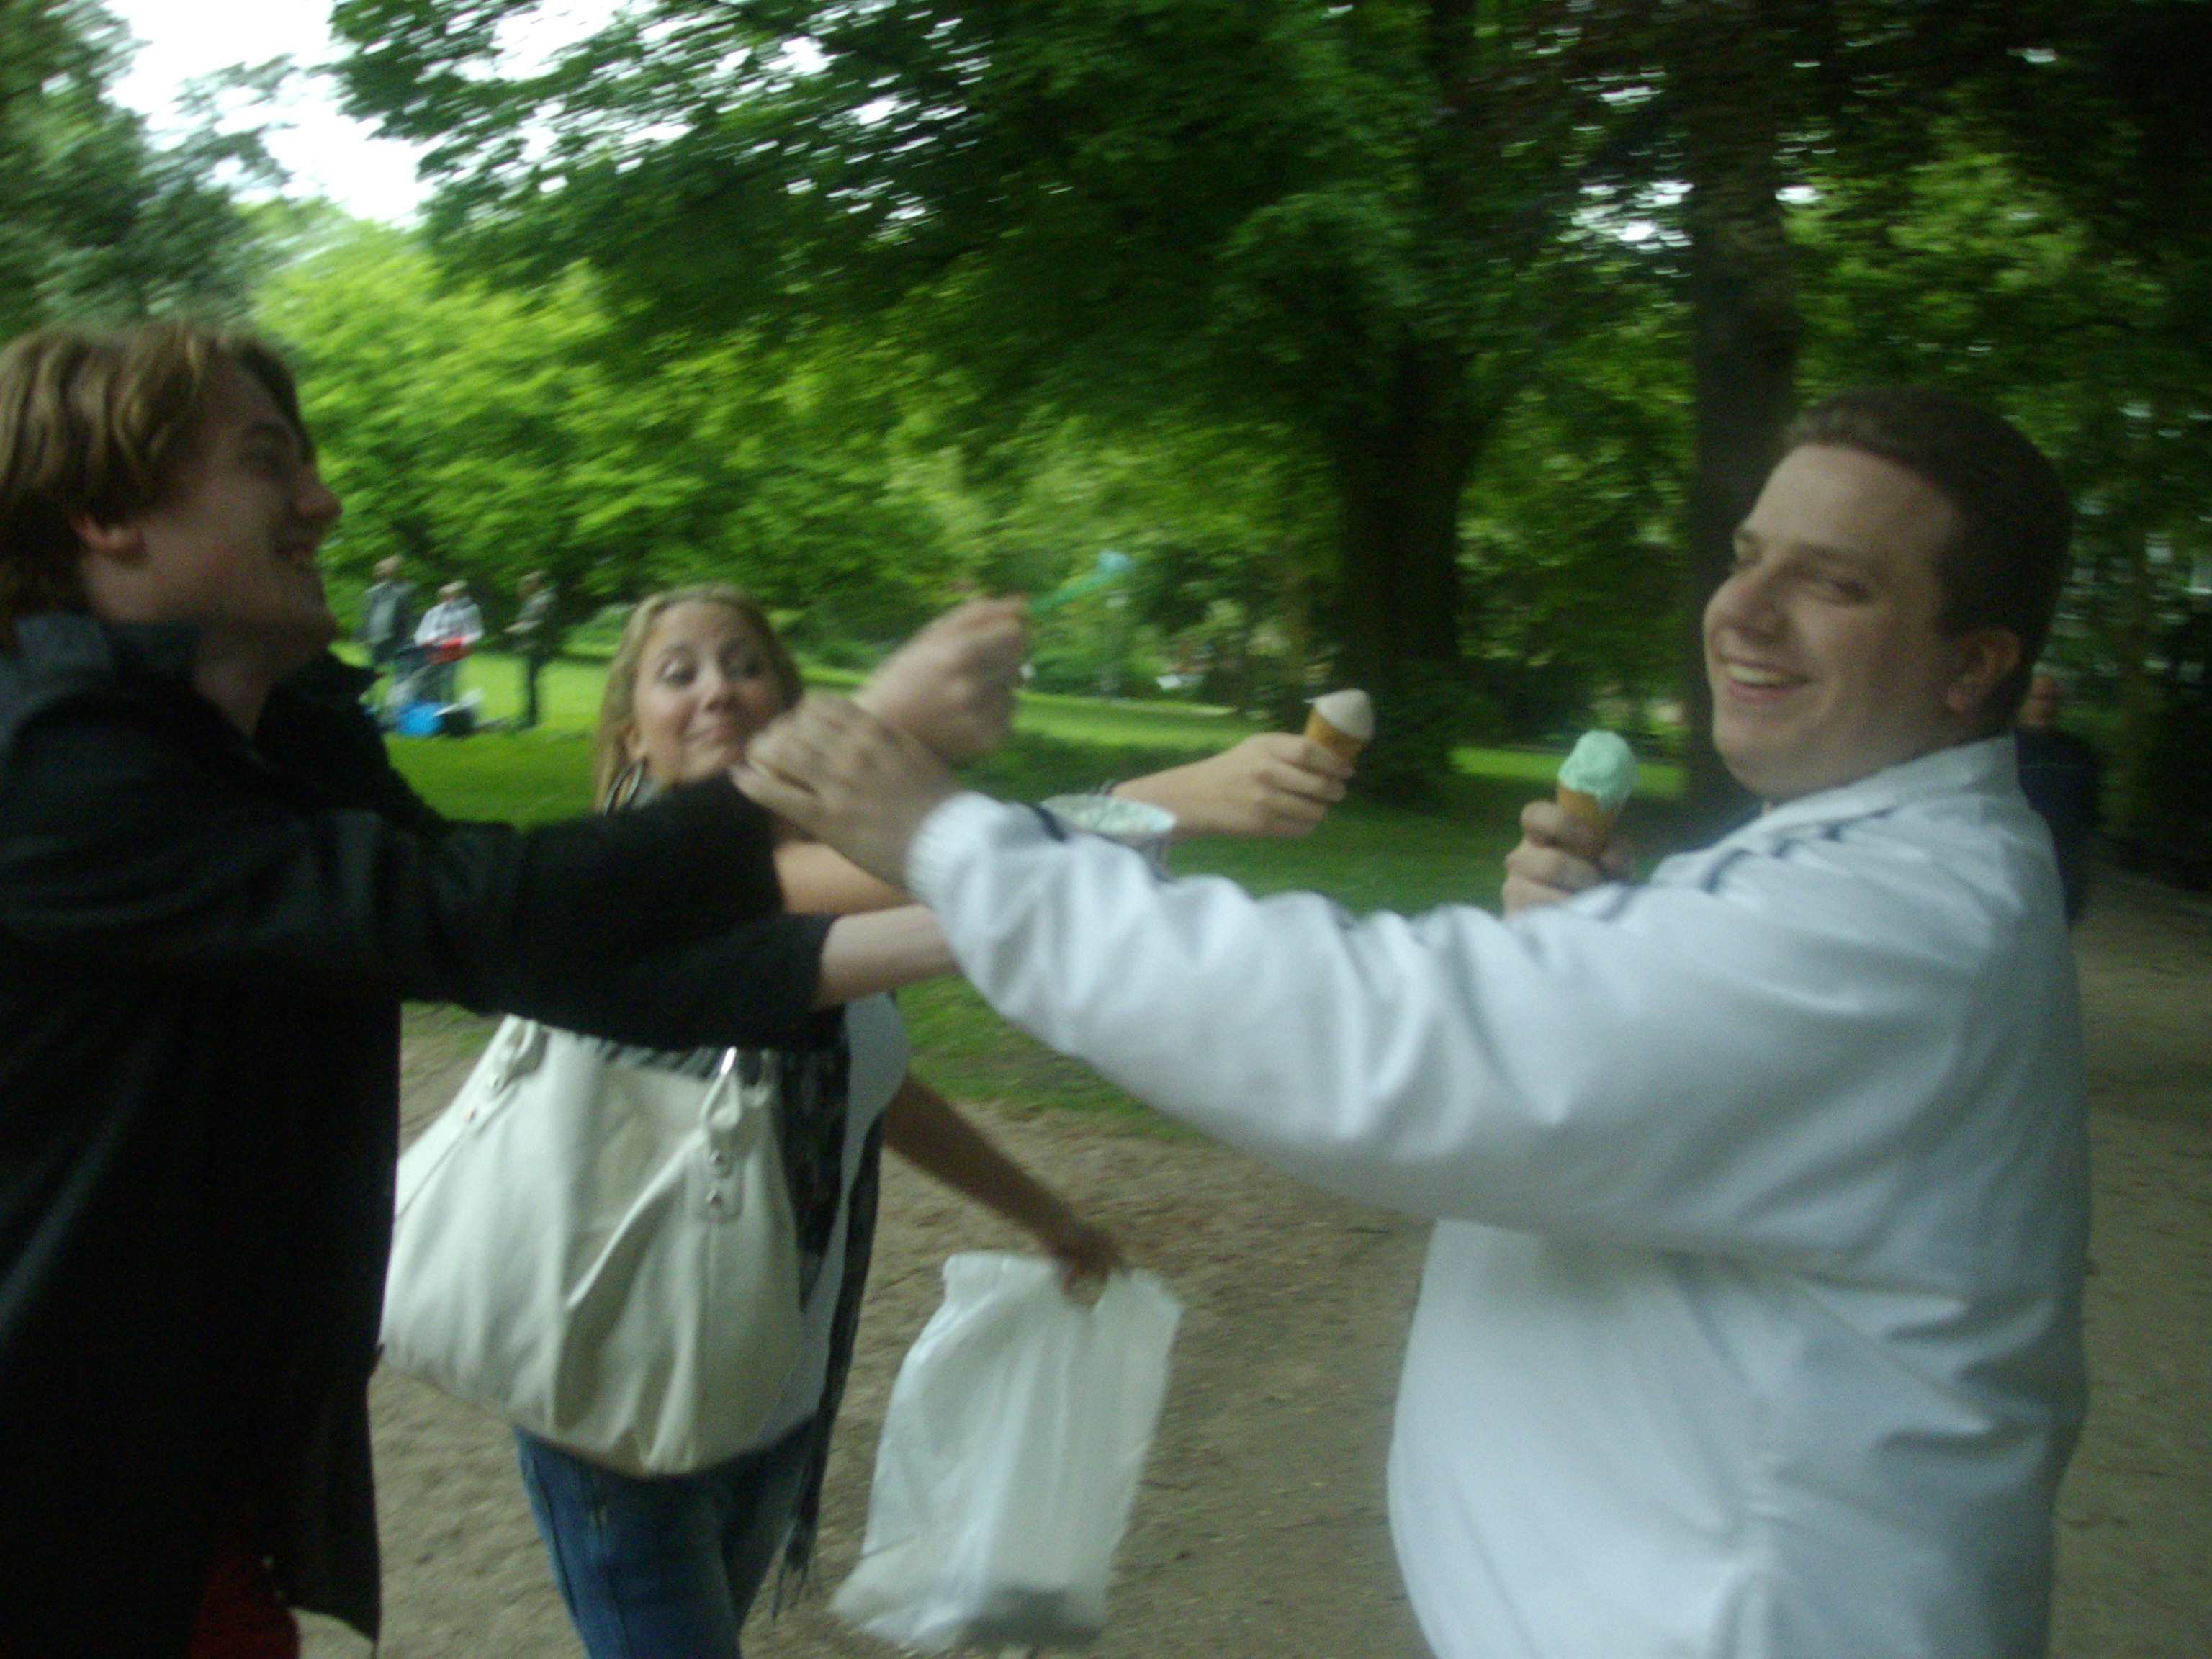
\includegraphics[width=.33\textwidth]{images/0302.jpg}%
        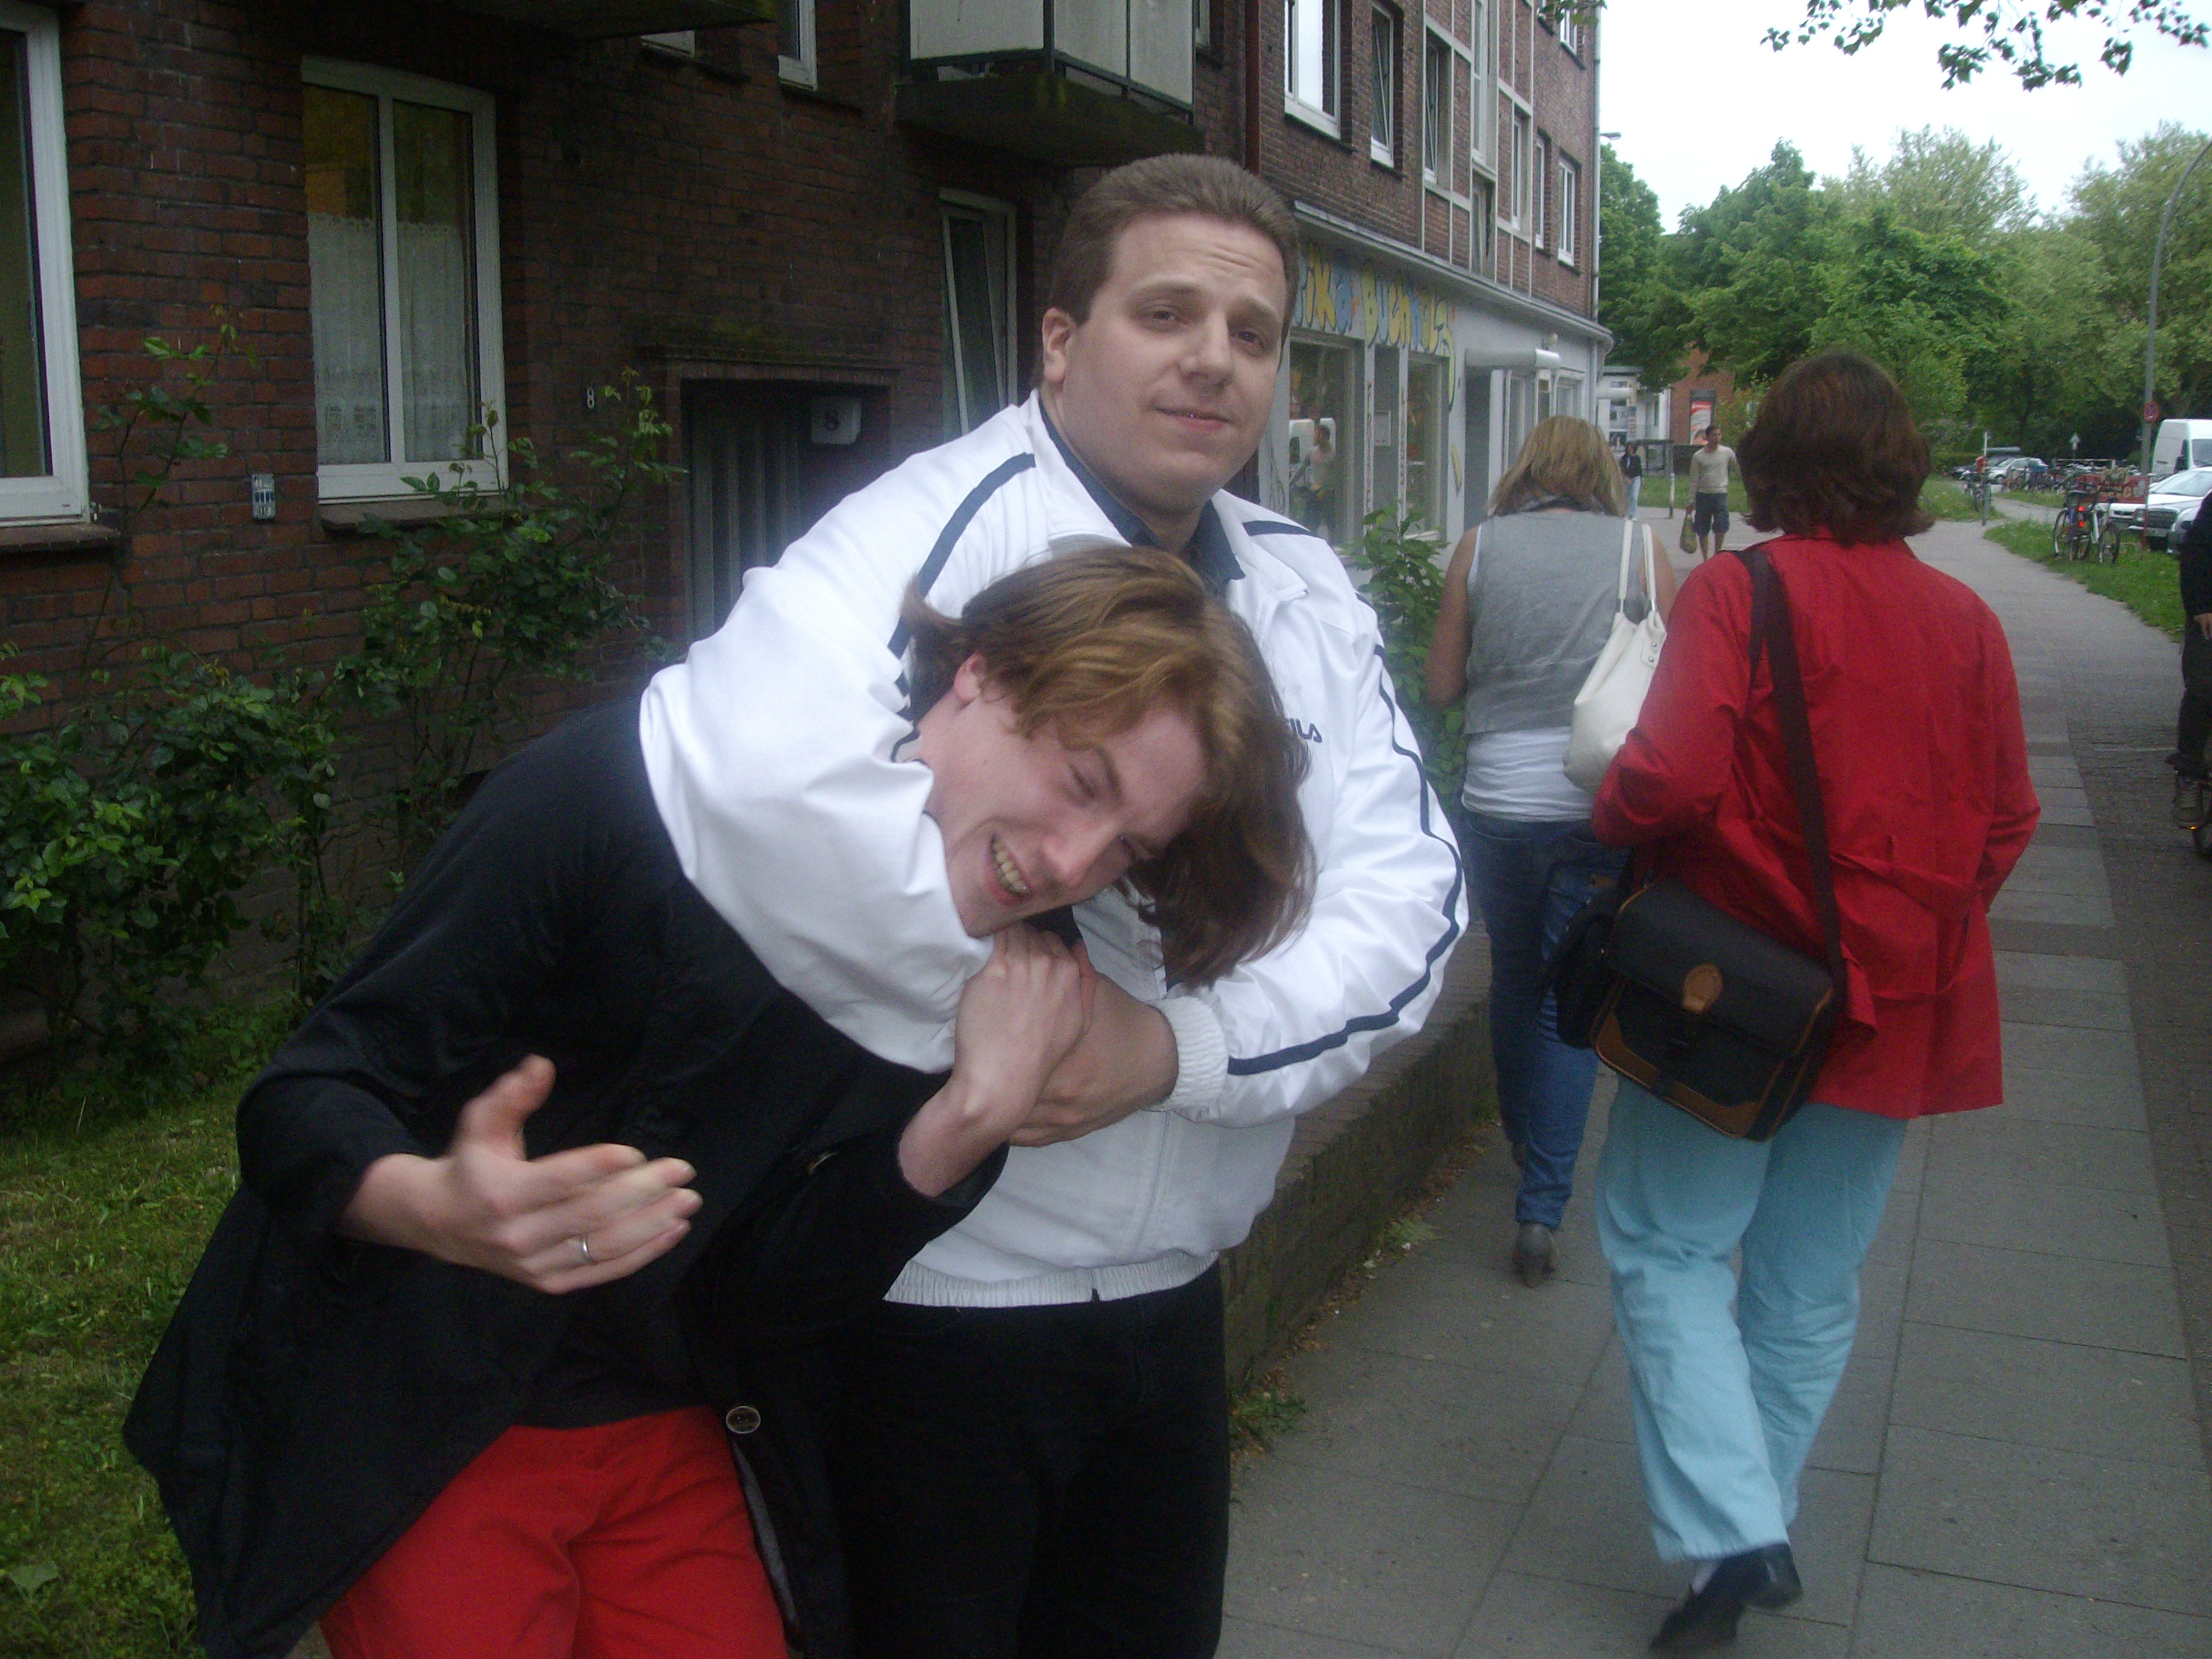
\includegraphics[width=.33\textwidth]{images/0303.jpg}
    \end{minipage}%
    \begin{minipage}{.17\textwidth}
        \centering
        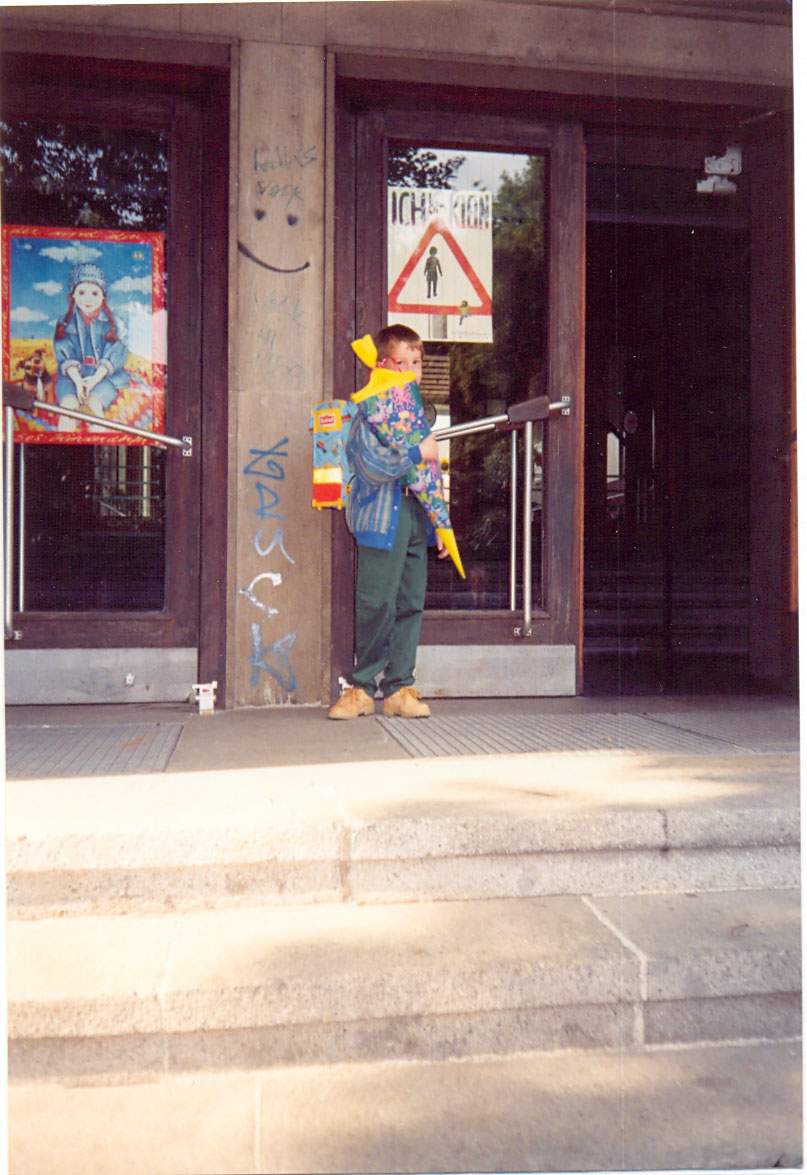
\includegraphics[width=1.0\textwidth]{images/0204.jpg}
        %\\
        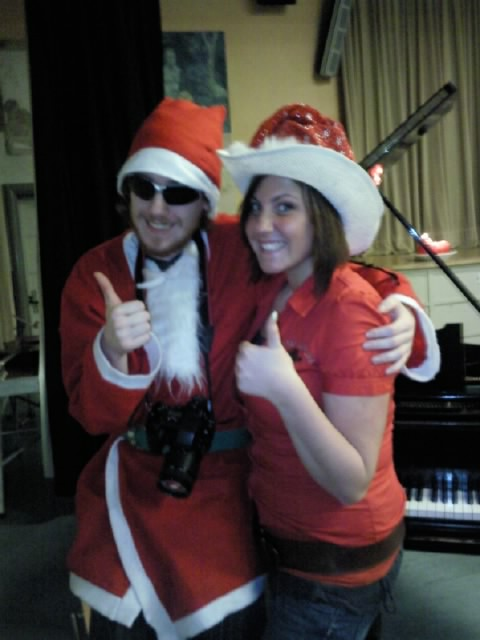
\includegraphics[width=1.0\textwidth]{images/0304.jpg}
    \end{minipage}
\end{frame}

% #############################################################################
\section{Bachelor}
\begin{frame}[fragile]
	\frametitle{Bachelor's Thesis (2022) I}
    \begin{itemize}
        \item Title: Perceptual Quality Assessment of Lip-Synchrony in Dubbing
    \end{itemize}
    \begin{minipage}{.5\textwidth}
      \begin{figure}
        \centering
        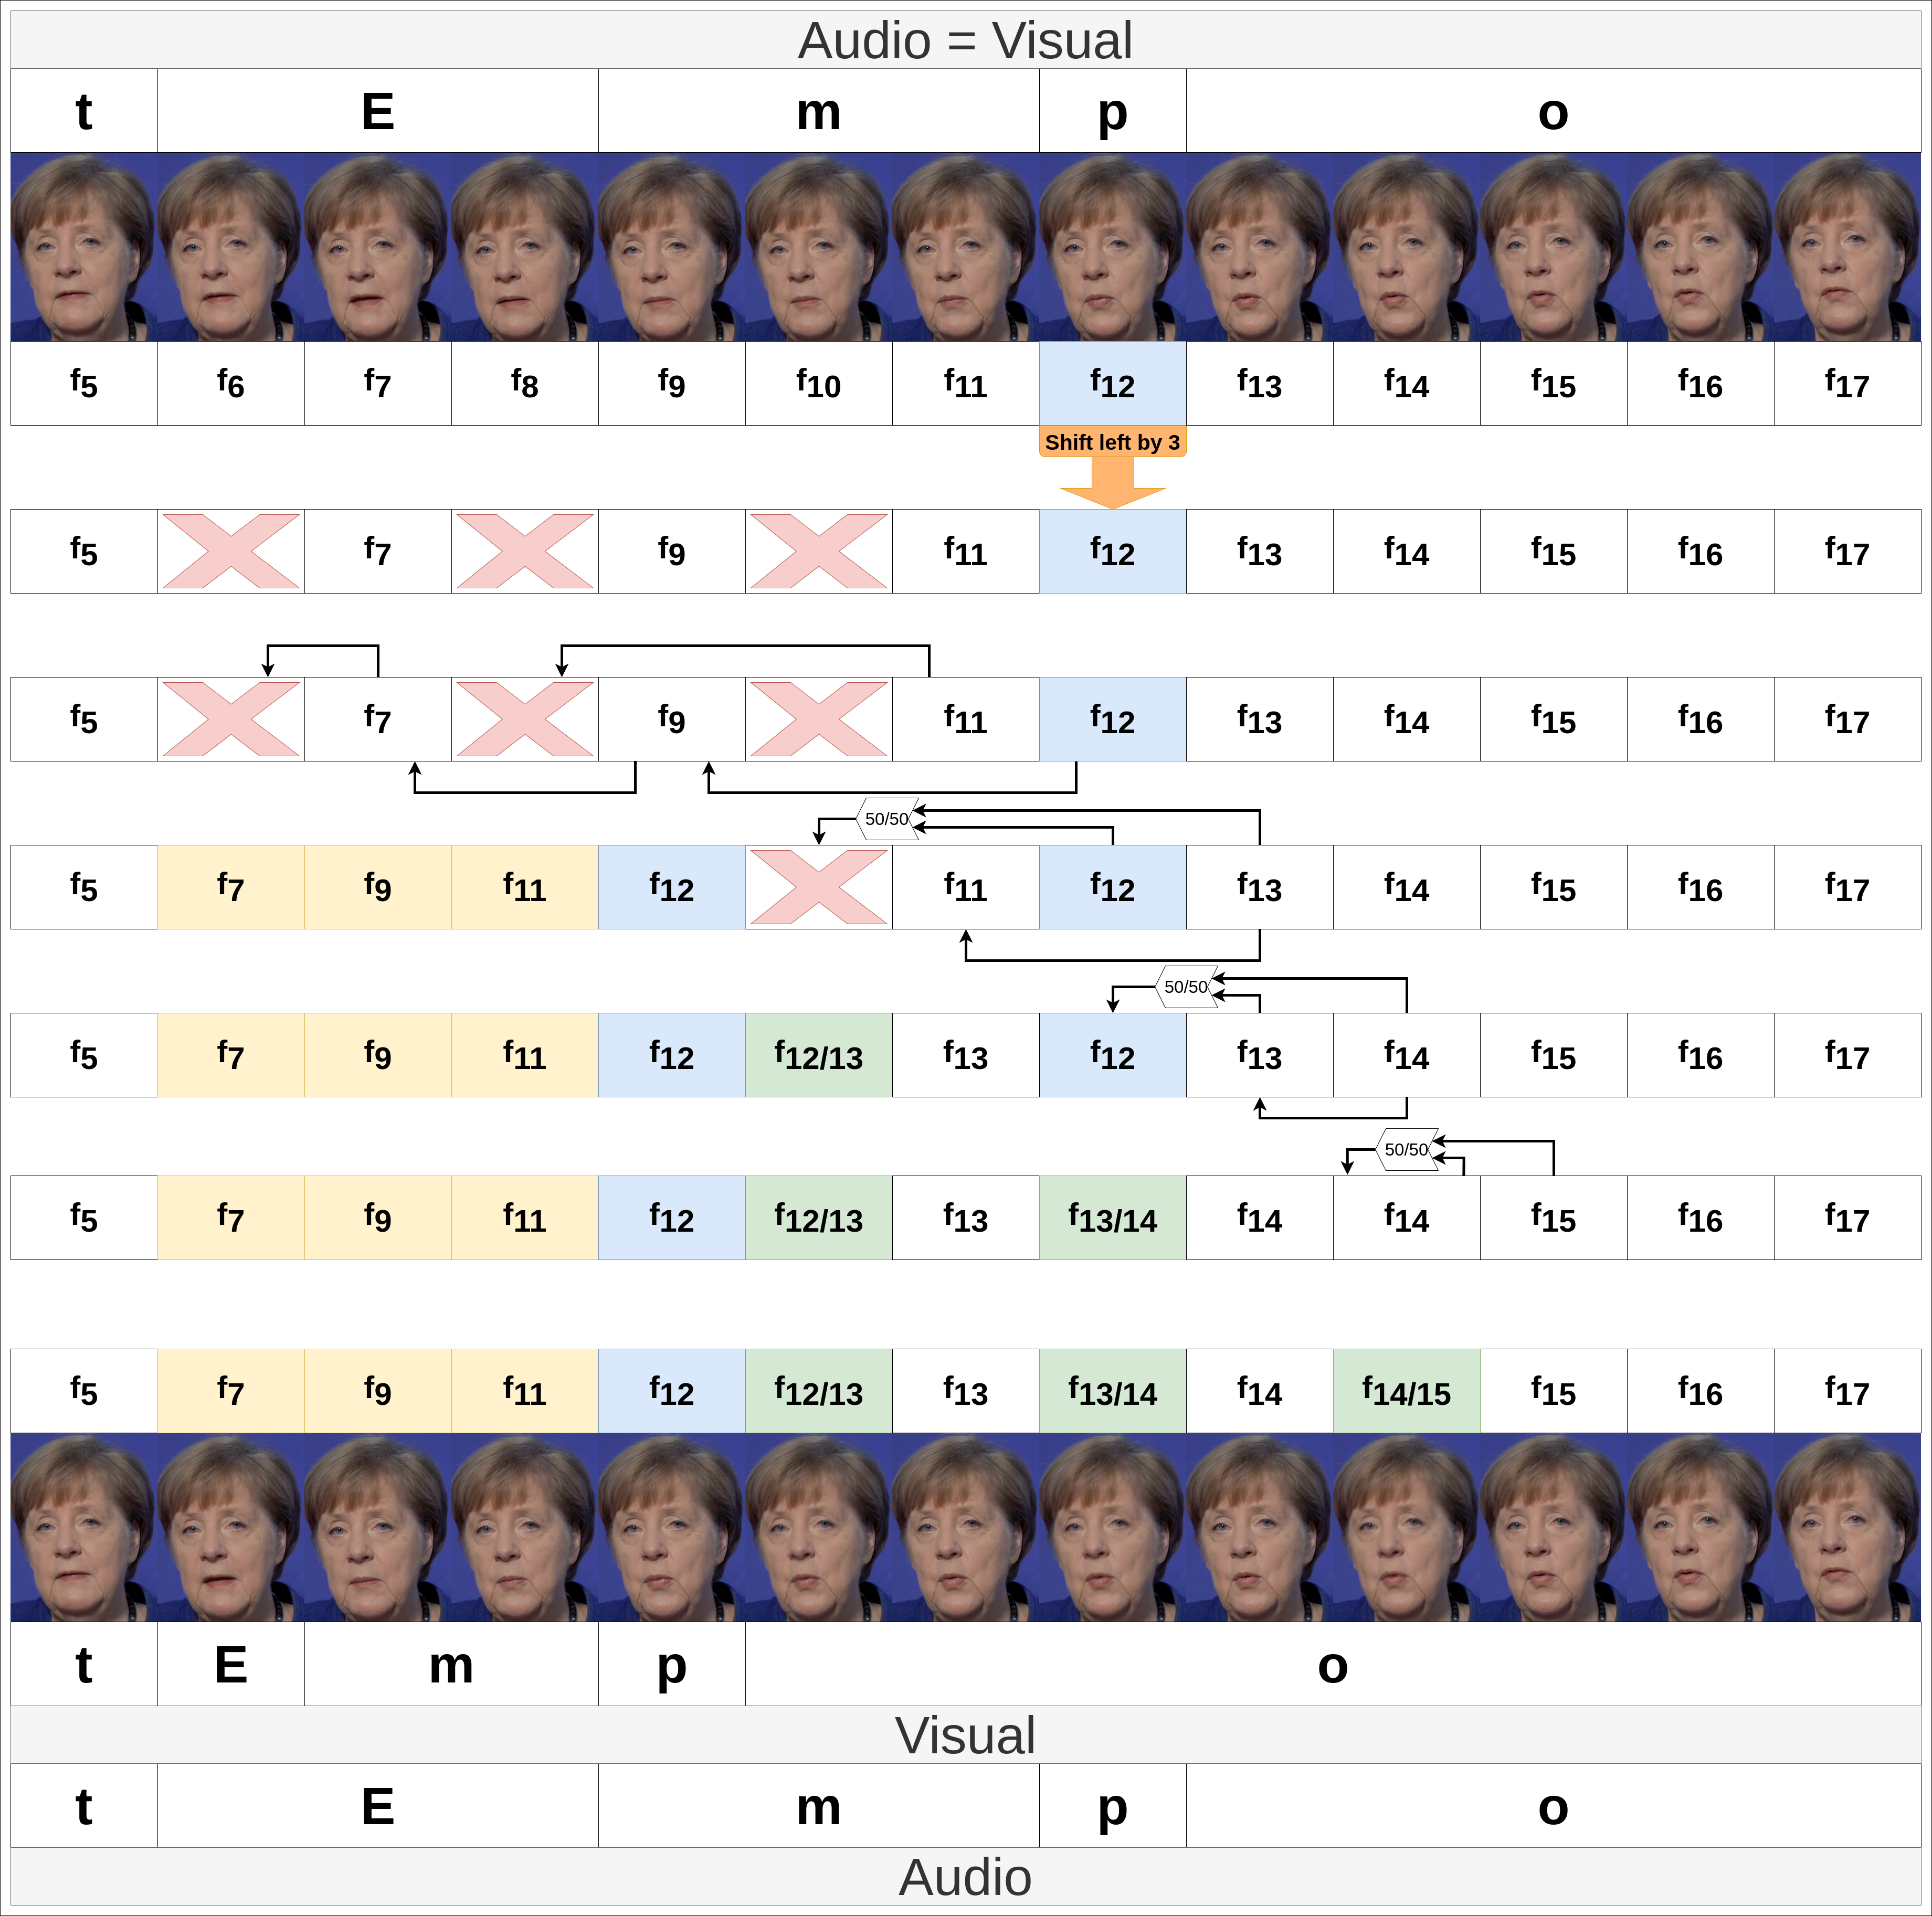
\includegraphics[width=.9\textwidth]{images/DubbingThesisEditing-vL-merkl.png} 
    \end{figure}
    \end{minipage}%
    \begin{minipage}{.5\textwidth}
    \centering
        \begin{minipage}{.3\textwidth}
            \centering
            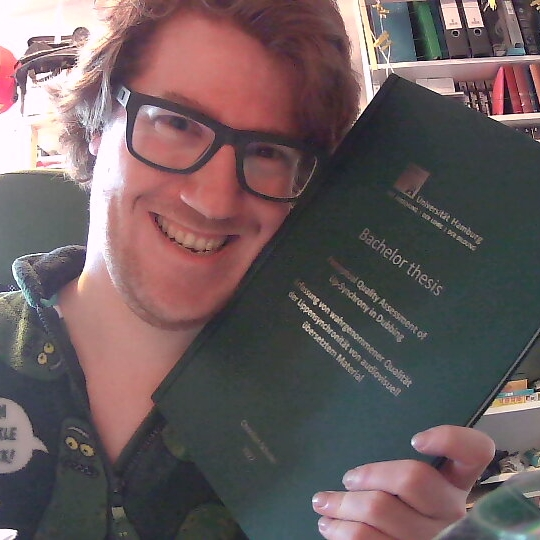
\includegraphics[height=2cm]{images/Christian_Schuler_Thesis.jpg} 
            \small{Christian Schuler}
        \end{minipage}%
        \begin{minipage}{.3\textwidth}
            \centering
            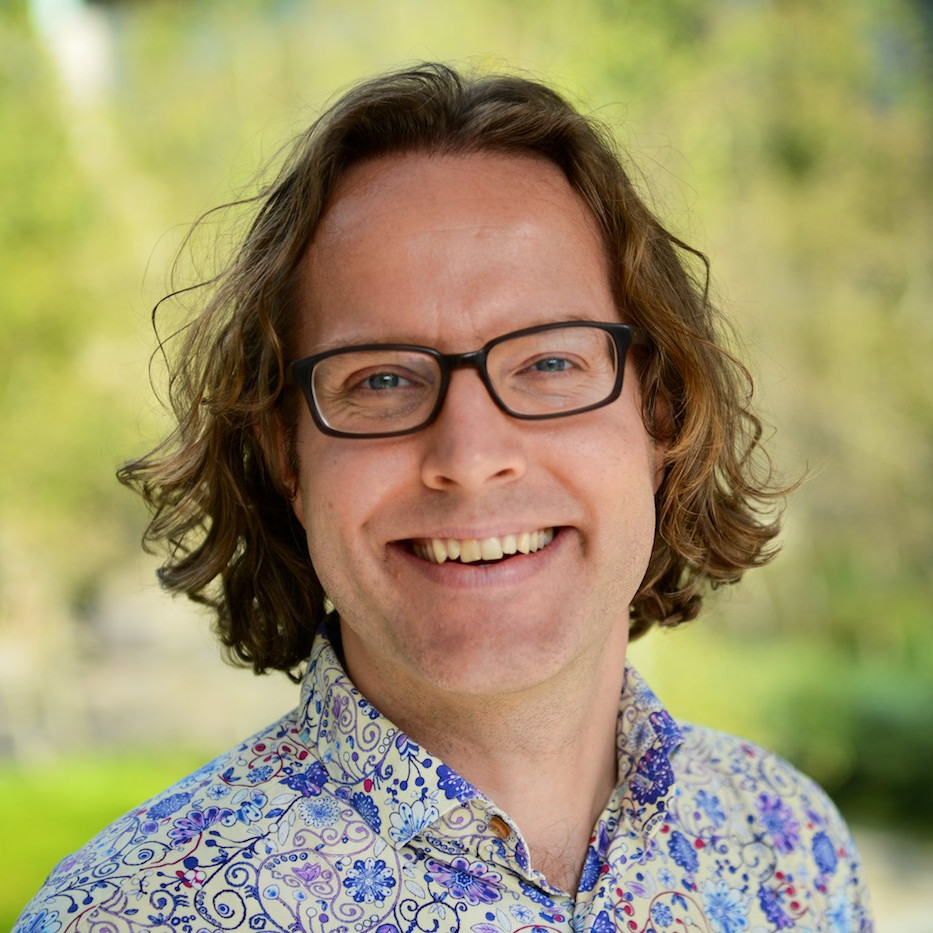
\includegraphics[height=2cm]{images/Timo_Baumann.jpg}
            \small{Dr. Timo Baumann}$^{*}$
        \end{minipage}%
        \begin{minipage}{.3\textwidth}
            \centering
            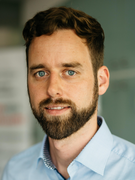
\includegraphics[height=2cm]{images/Timo_Florian_Gerkmann.png}
            \small{Prof. Timo Gerkmann}
        \end{minipage}
    \end{minipage}
    \begin{minipage}{0.9\textwidth}
        \hfill $^{*}$ since 2022 Professor.
    \end{minipage}
\end{frame}

\begin{frame}[fragile]
	\frametitle{Bachelor's Thesis (2022) II}
    \begin{minipage}{.4\textwidth}
        \centering
        \textbf{Study Setup}
        \begin{figure}
            \centering
            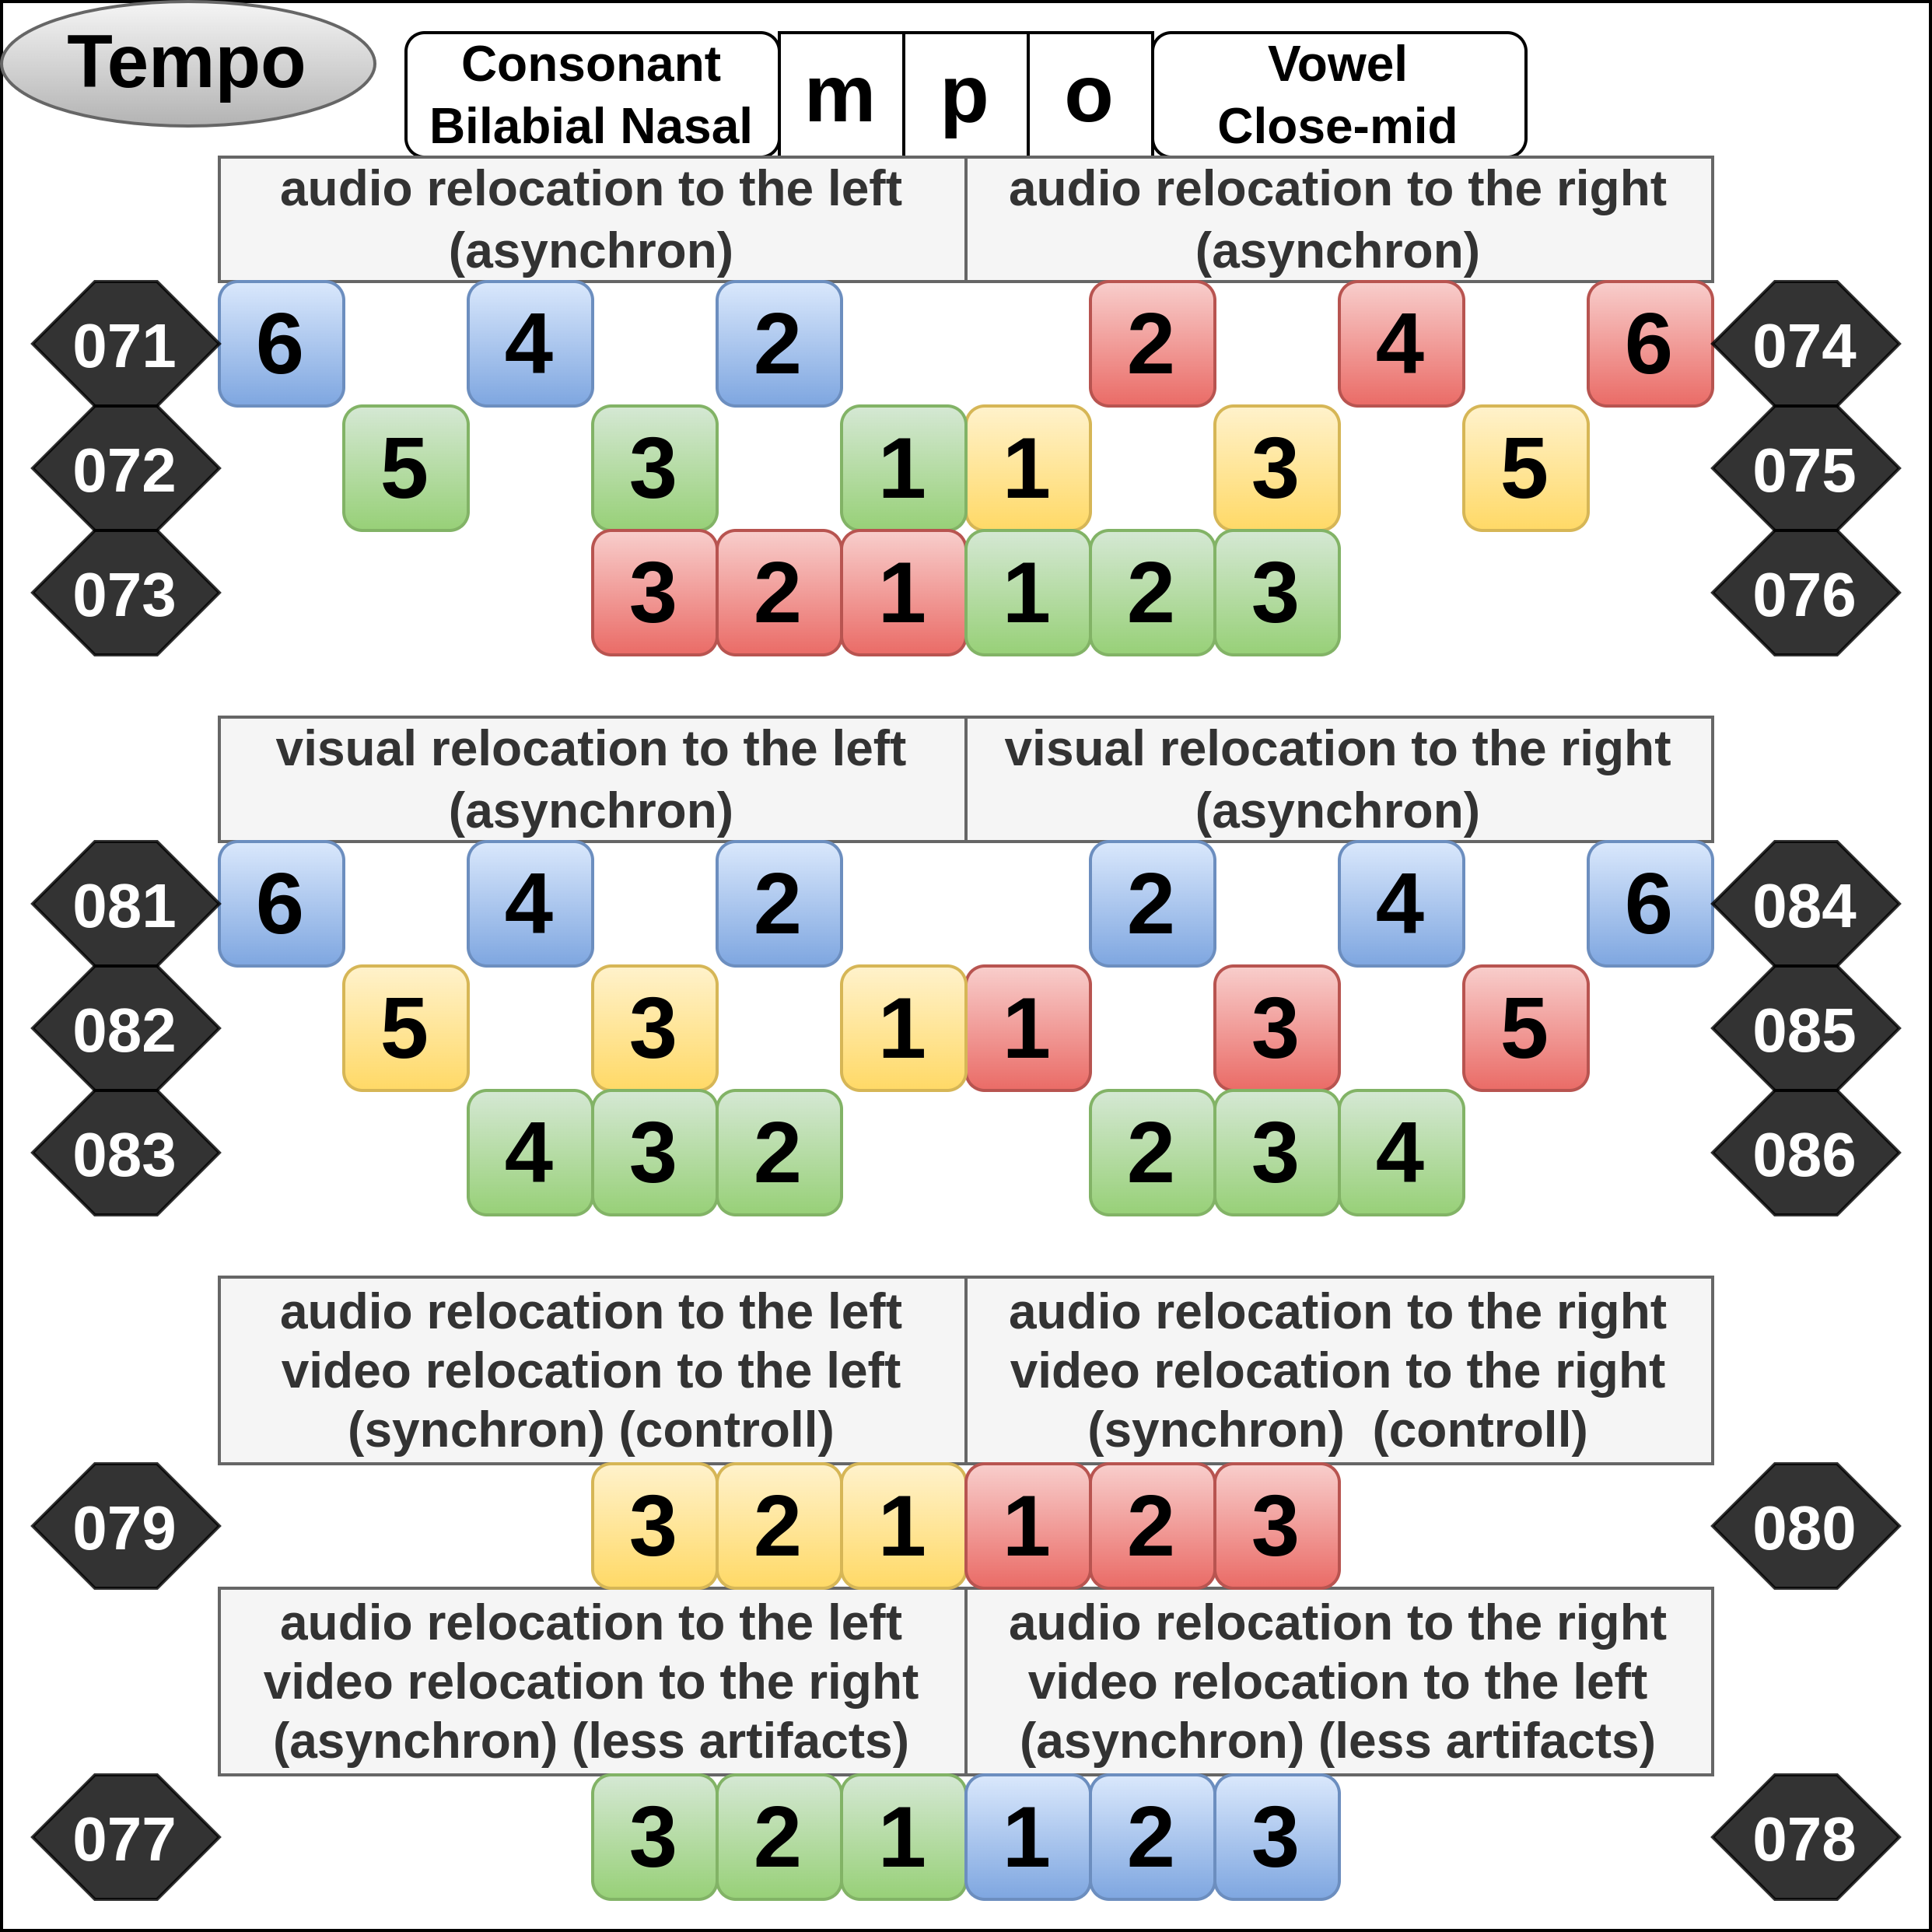
\includegraphics[width=.9\textwidth]{images/DubbingThesisTrials-sessionSingle.png} 
        \end{figure}
    \end{minipage}%
    \begin{minipage}{.6\textwidth}
        \centering
        \textbf{Anchor Items}
        \begin{figure}
            \centering
            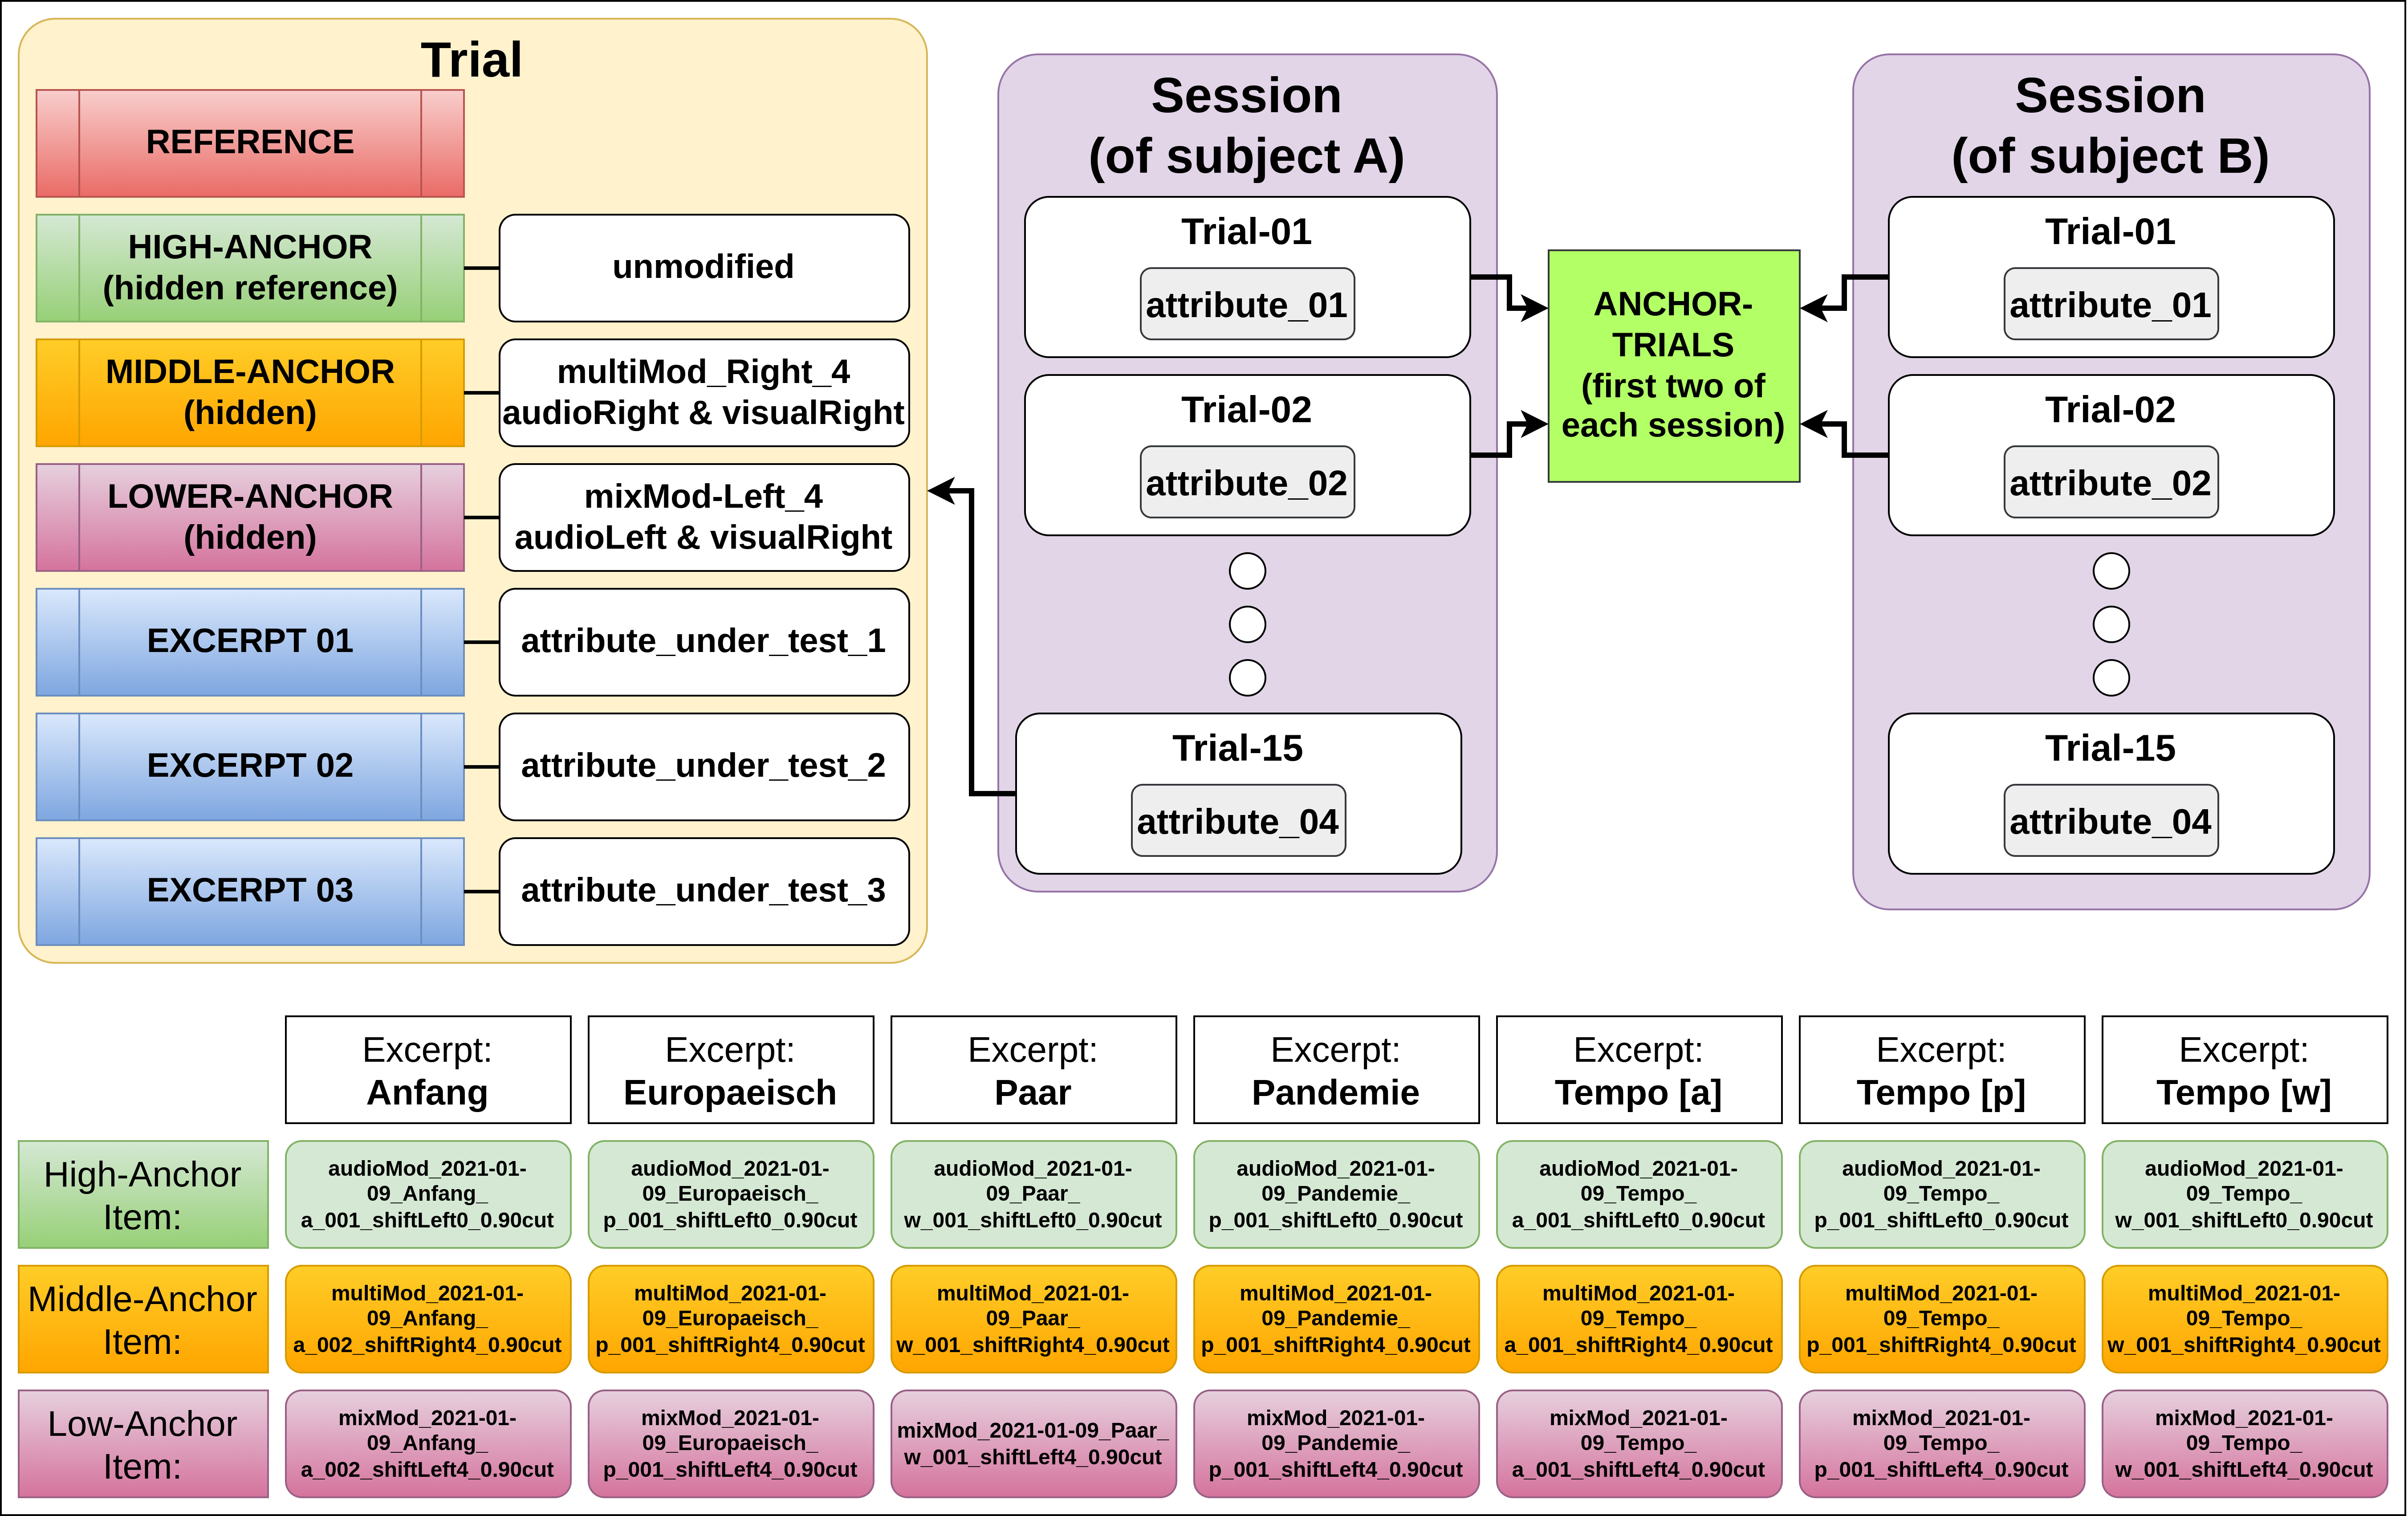
\includegraphics[width=1.0\textwidth]{images/DubbingThesisTrials-trialsConcept.png} 
        \end{figure}
    \end{minipage}
\end{frame}


\begin{frame}[fragile]
	\frametitle{Bachelor's Thesis Fallout I}
    \begin{minipage}{.63\textwidth}
        %\textbf{Linux Articles}\\
        {\color{thiscolor}$\bullet$} Natural Language Processing mit Neuronalen Netzen 
        \\ \citep{baumann2022NaturalLanguageProcessing} Linux Article
        \\ {\color{thiscolor}$\bullet$} Lip-Synched 
        \\ \citep{baumann2023LipSynchedLinuxMagazine} Linux Article
        
        \begin{minipage}{1.0\textwidth}
            \centering
                \begin{minipage}{.3\textwidth}
                    \centering
                    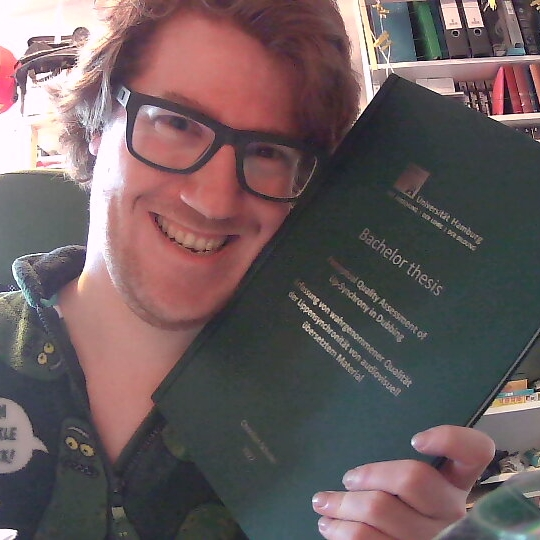
\includegraphics[height=2cm]{images/Christian_Schuler_Thesis.jpg} 
                    %\\ 
                    Christian
                \end{minipage}
                \begin{minipage}{.3\textwidth}
                    \centering
                    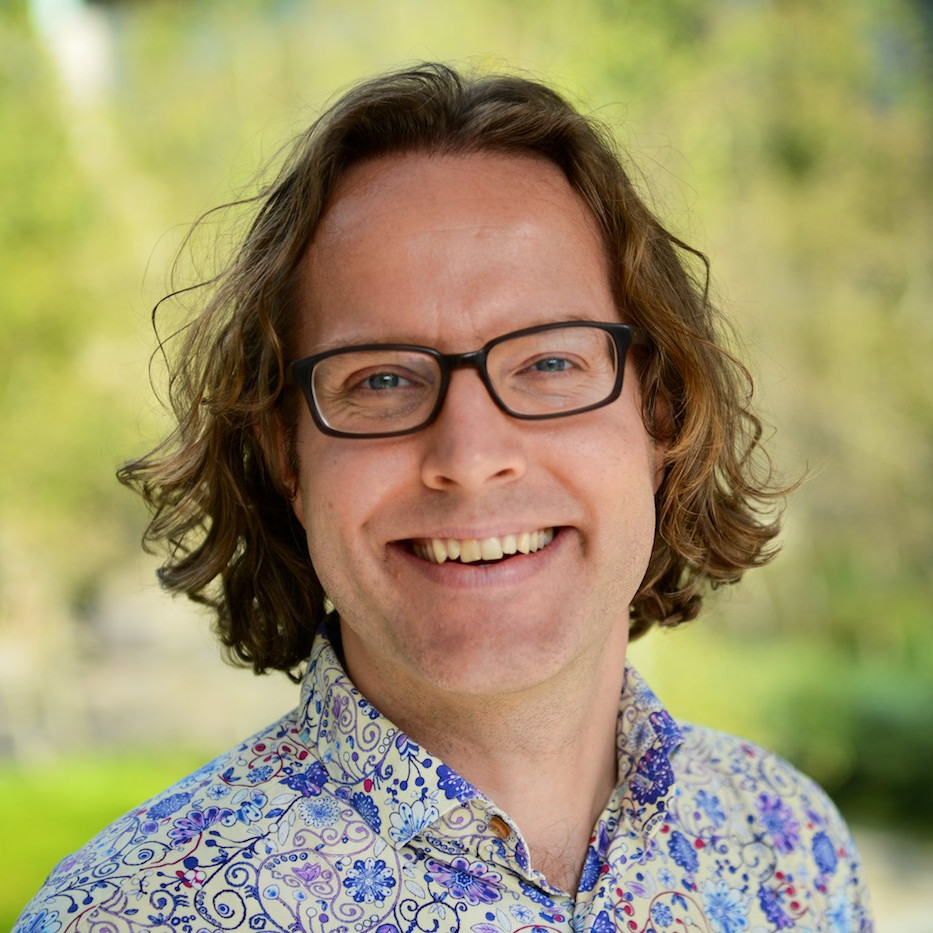
\includegraphics[height=2cm]{images/Timo_Baumann.jpg}
                    %\\ 
                    Timo
                \end{minipage}
        \end{minipage}
        % \begin{figure}
        %     \centering
        %     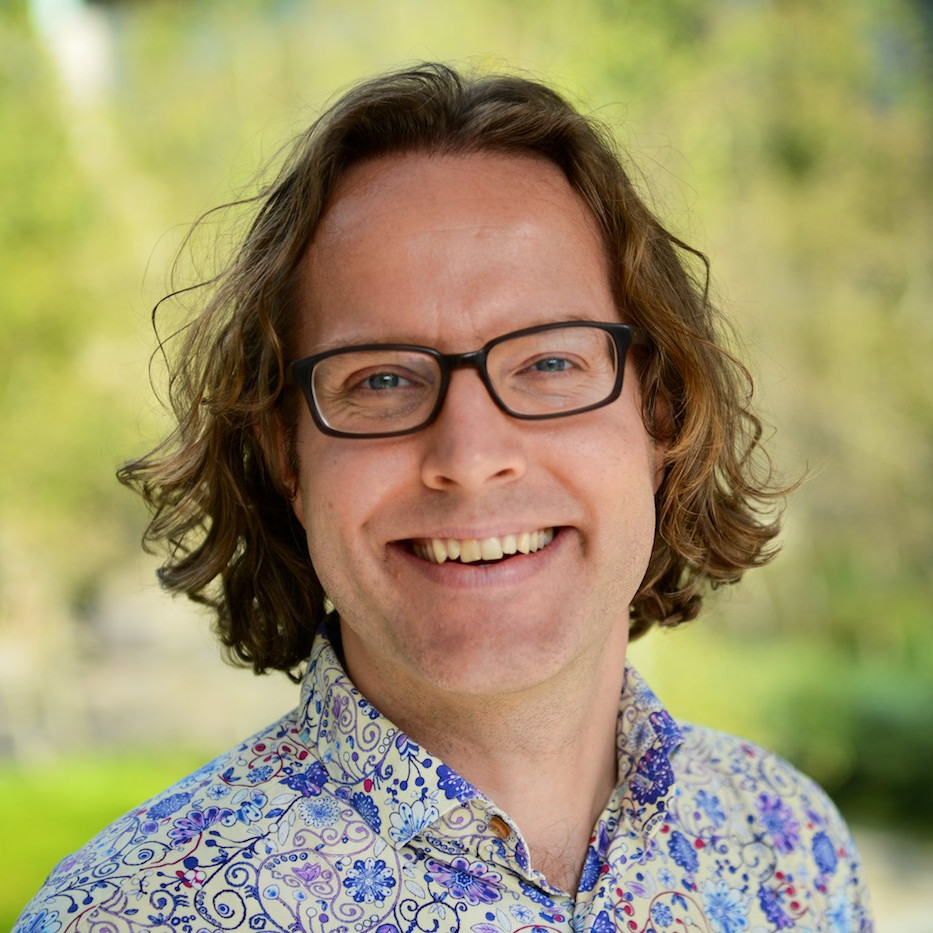
\includegraphics[width=0.3\textwidth]{images/Timo_Baumann.jpg}
        %     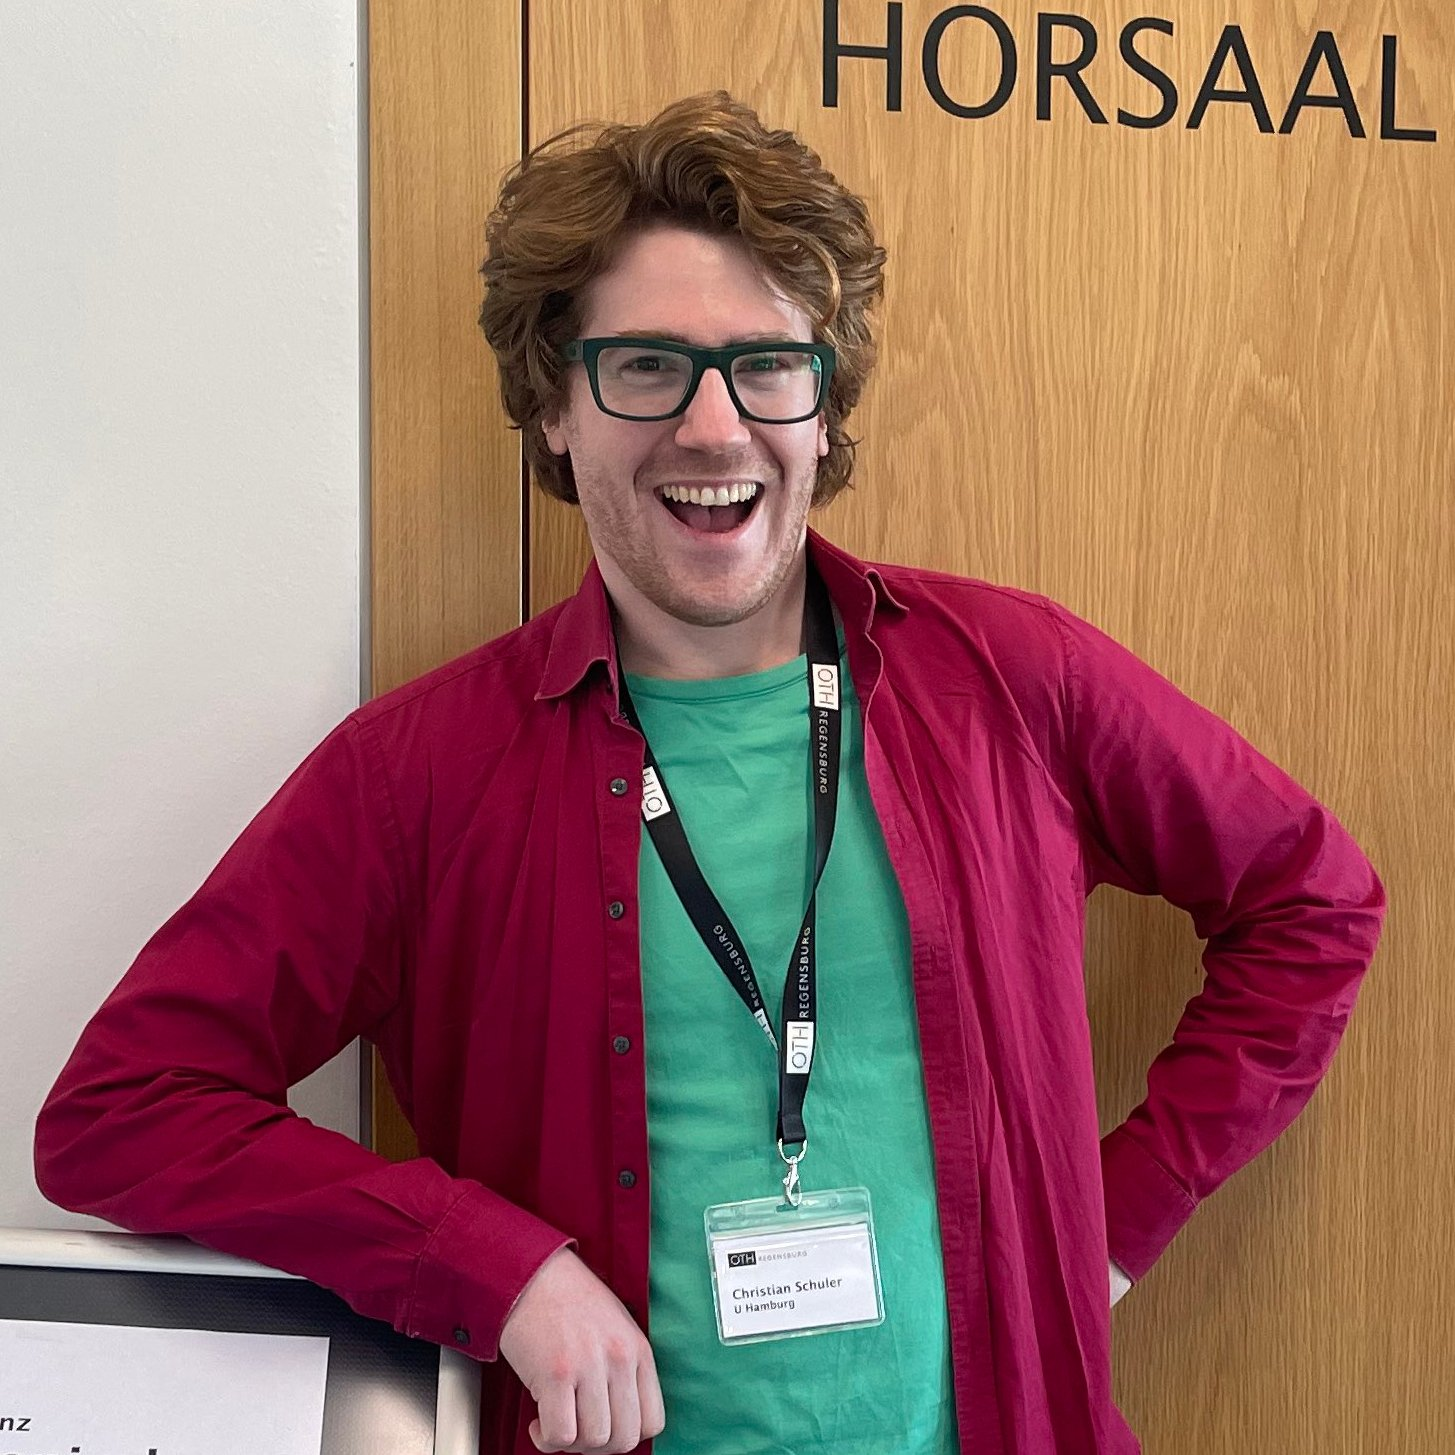
\includegraphics[width=0.3\textwidth]{images/Christian_Schuler_Essv.jpg}
        % \end{figure}
    \end{minipage}\hfill%
    \begin{minipage}{.32\textwidth}
        {\color{thiscolor}$\bullet$} StudyToolkitVid
        \\ A toolkit for creating studies to evaluate quality of videos.
        \centering
        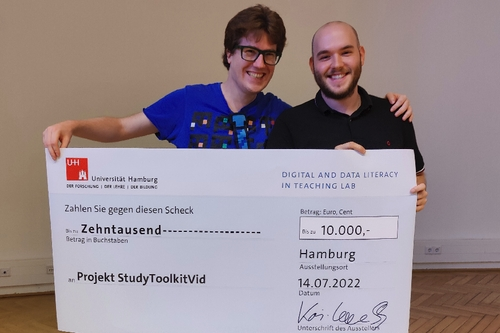
\includegraphics[width=1.0\textwidth]{images/proj-2022-ddlitlab-StudyToolkitVid-500x333.jpg} 
        Christian \& Dominik
        % \begin{figure}
        % \centering
        % 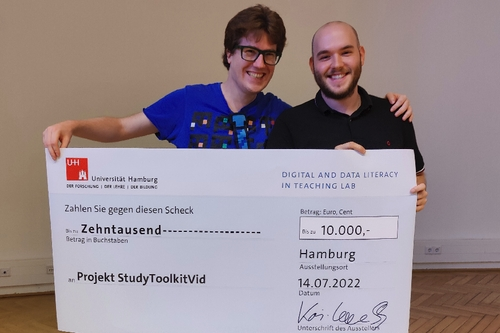
\includegraphics[width=0.8\textwidth]{images/proj-2022-ddlitlab-StudyToolkitVid-500x333.jpg} 
        % \end{figure}
    \end{minipage}
\end{frame}

\begin{frame}[fragile]
	\frametitle{Bachelor's Thesis Fallout II}
    \begin{minipage}{1.0\textwidth}
        \begin{minipage}{.55\textwidth}
            \textbf{Neural audio-visual synchrony evaluation}
            \par\noindent\rule{\textwidth}{0.4pt}
            {\color{thiscolor}$\bullet$} A Deep Dive Into Neural Synchrony Evaluation for Audio-visual Translation
            \\ \citep{nayak2022DeepDiveNeural}
            %\vspace{-8mm}
        \end{minipage}
        \begin{minipage}{.44\textwidth}
            \centering
            \begin{minipage}{.24\textwidth}
                \centering
                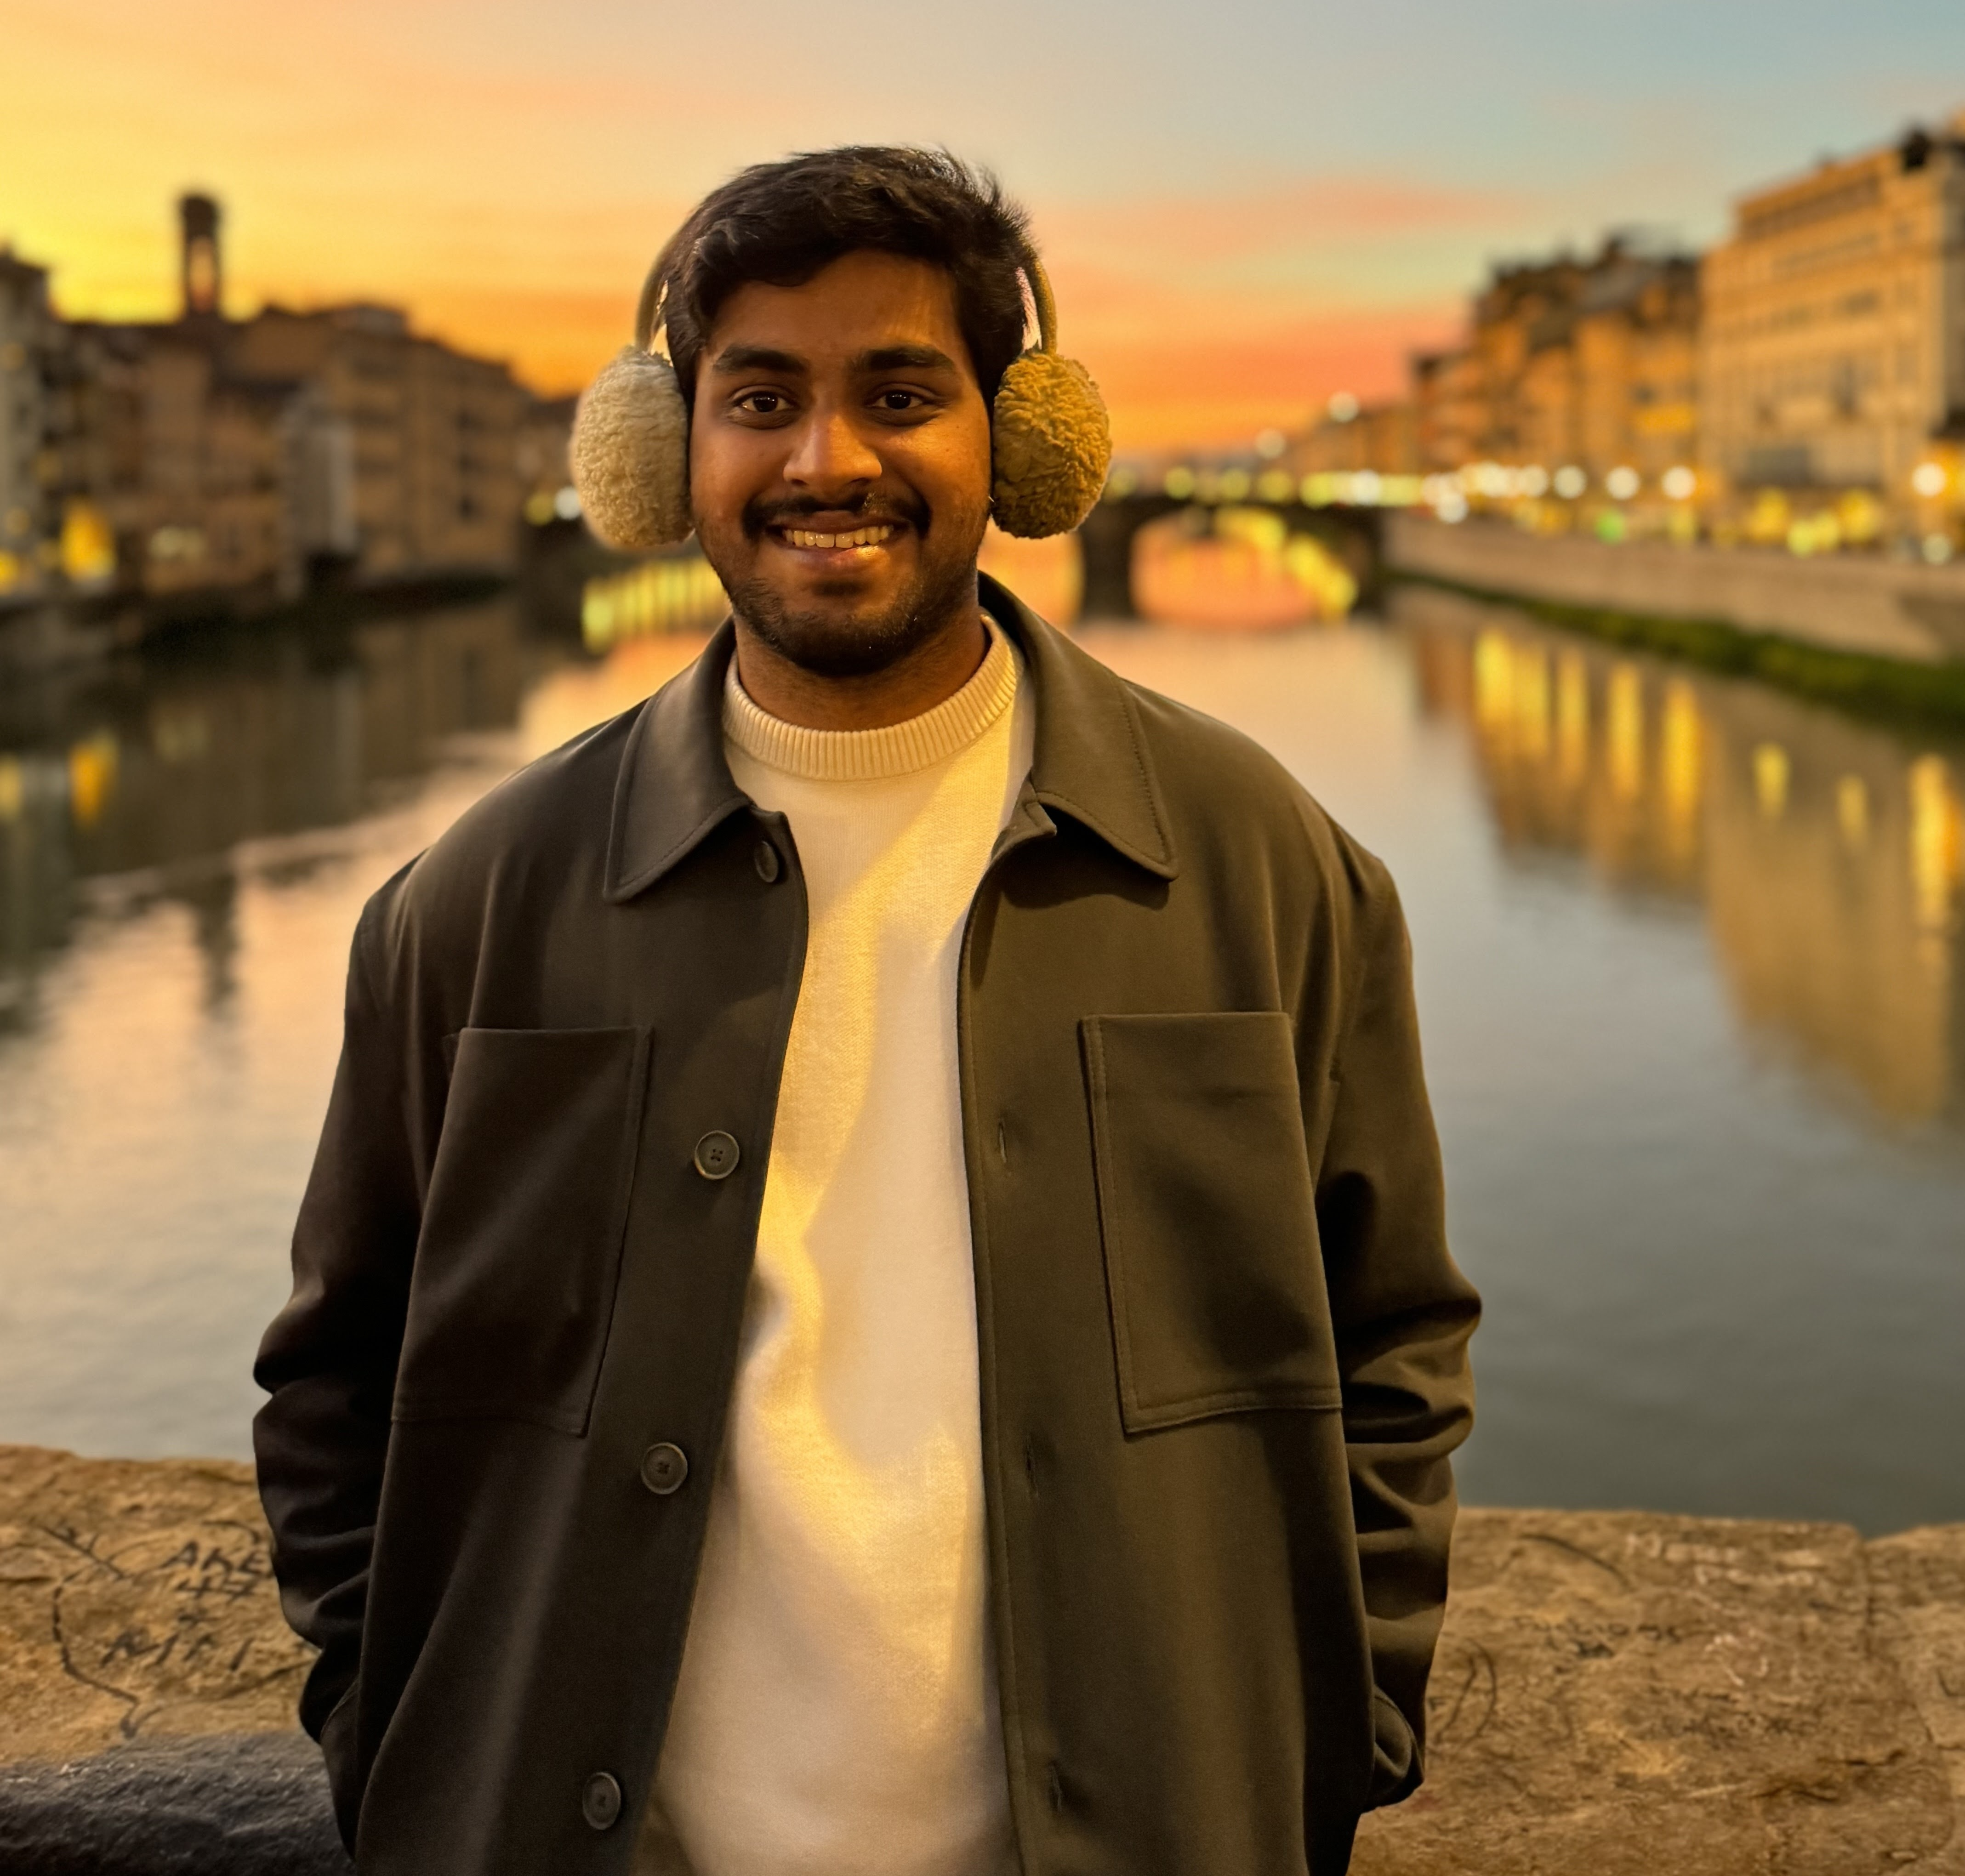
\includegraphics[height=1.4cm]{images/Shravan_Nayak.jpg} 
                Shravan
            \end{minipage}%
            \begin{minipage}{.24\textwidth}
                \centering
                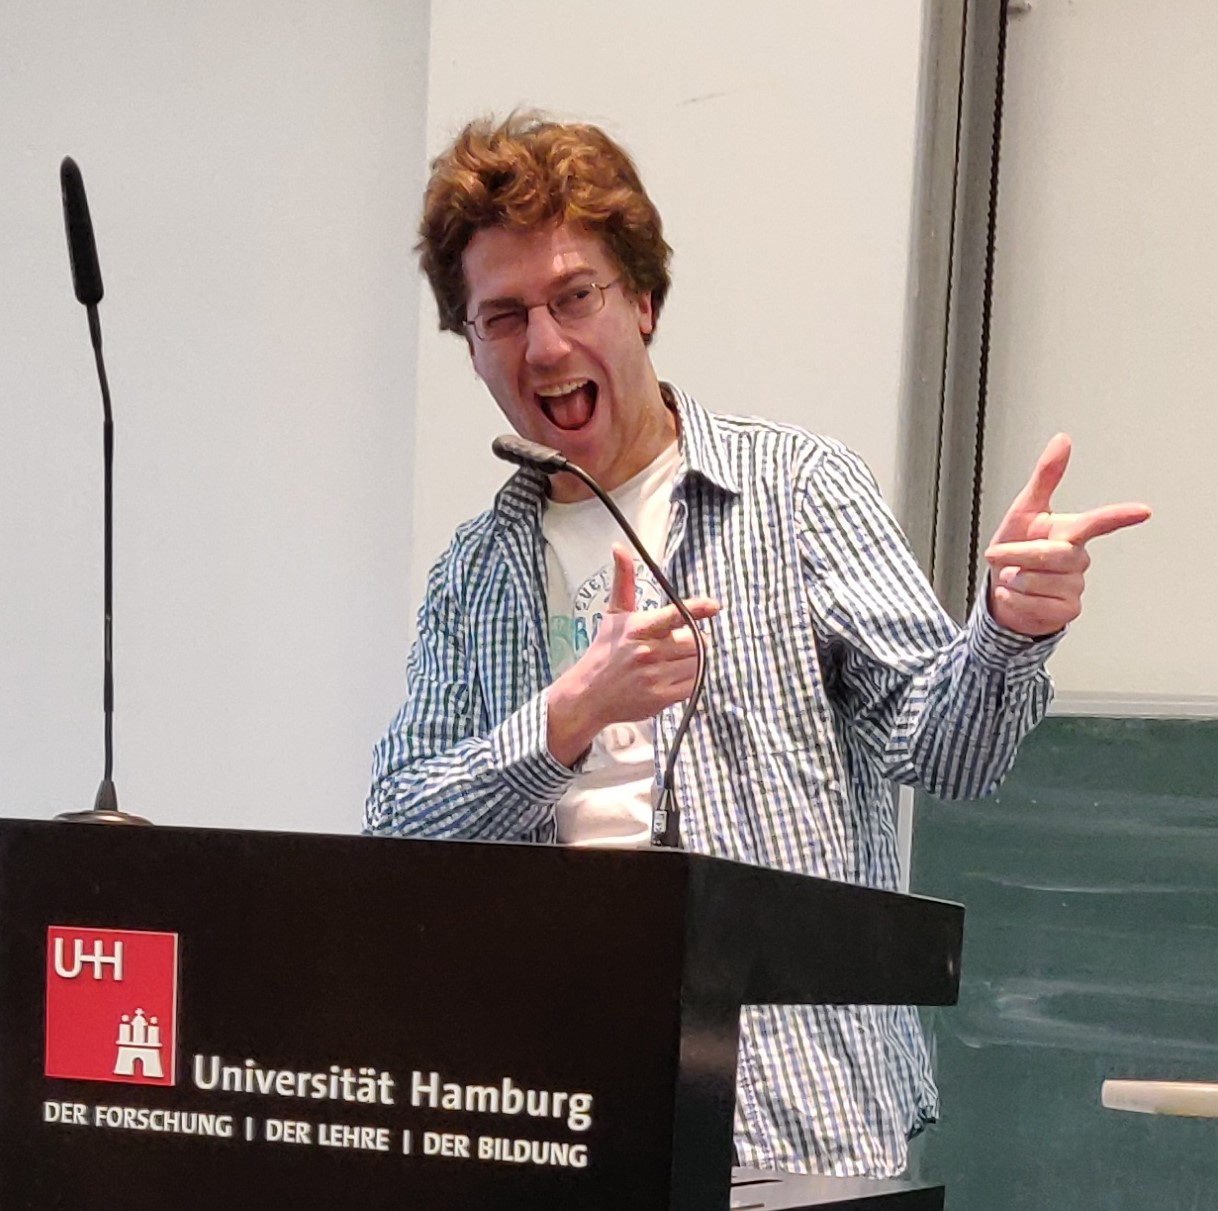
\includegraphics[height=1.4cm]{images/Christian_Schuler_Lecture.jpg}
                Christian
            \end{minipage}%
            \begin{minipage}{.24\textwidth}
                \centering
                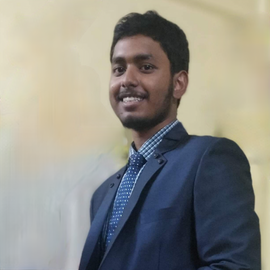
\includegraphics[height=1.4cm]{images/Debjoy_Saha.png}
                Debjoy
            \end{minipage}%
            \begin{minipage}{.24\textwidth}
                \centering
                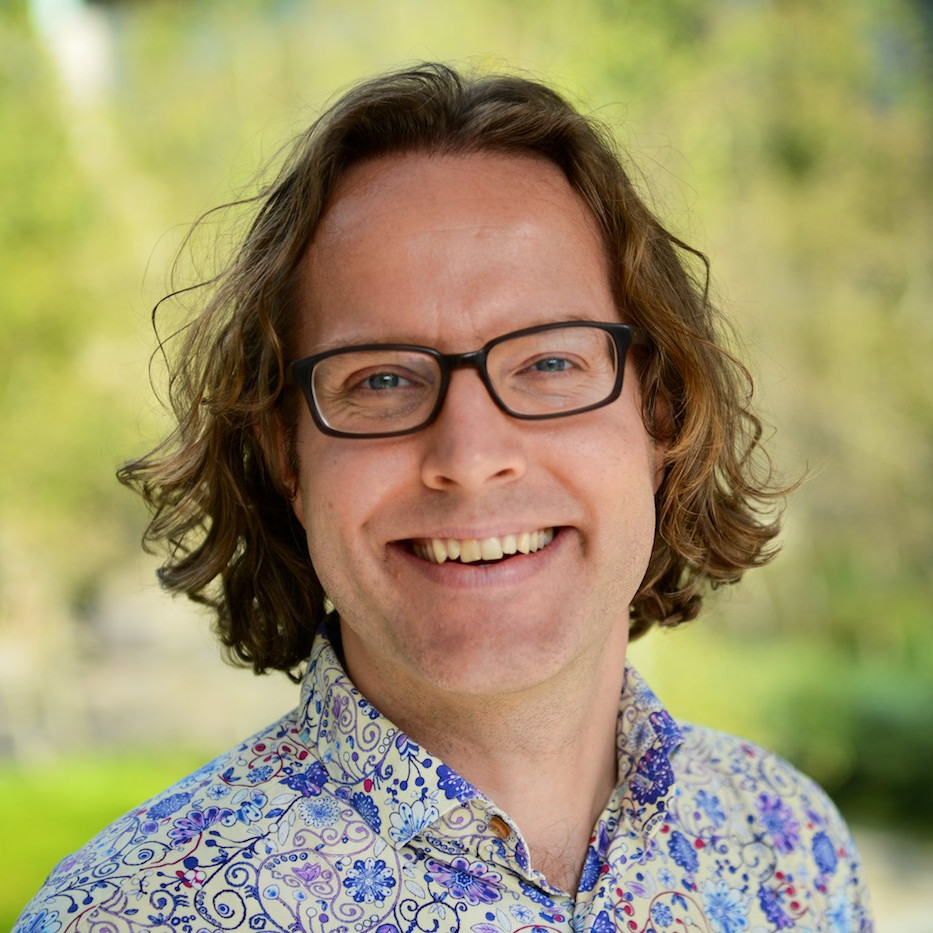
\includegraphics[height=1.4cm]{images/Timo_Baumann.jpg}
                Timo
            \end{minipage}
            % \begin{figure}
            % \centering
            % \captionsetup[subfigure]{labelformat=empty}
            %     \subfloat[]{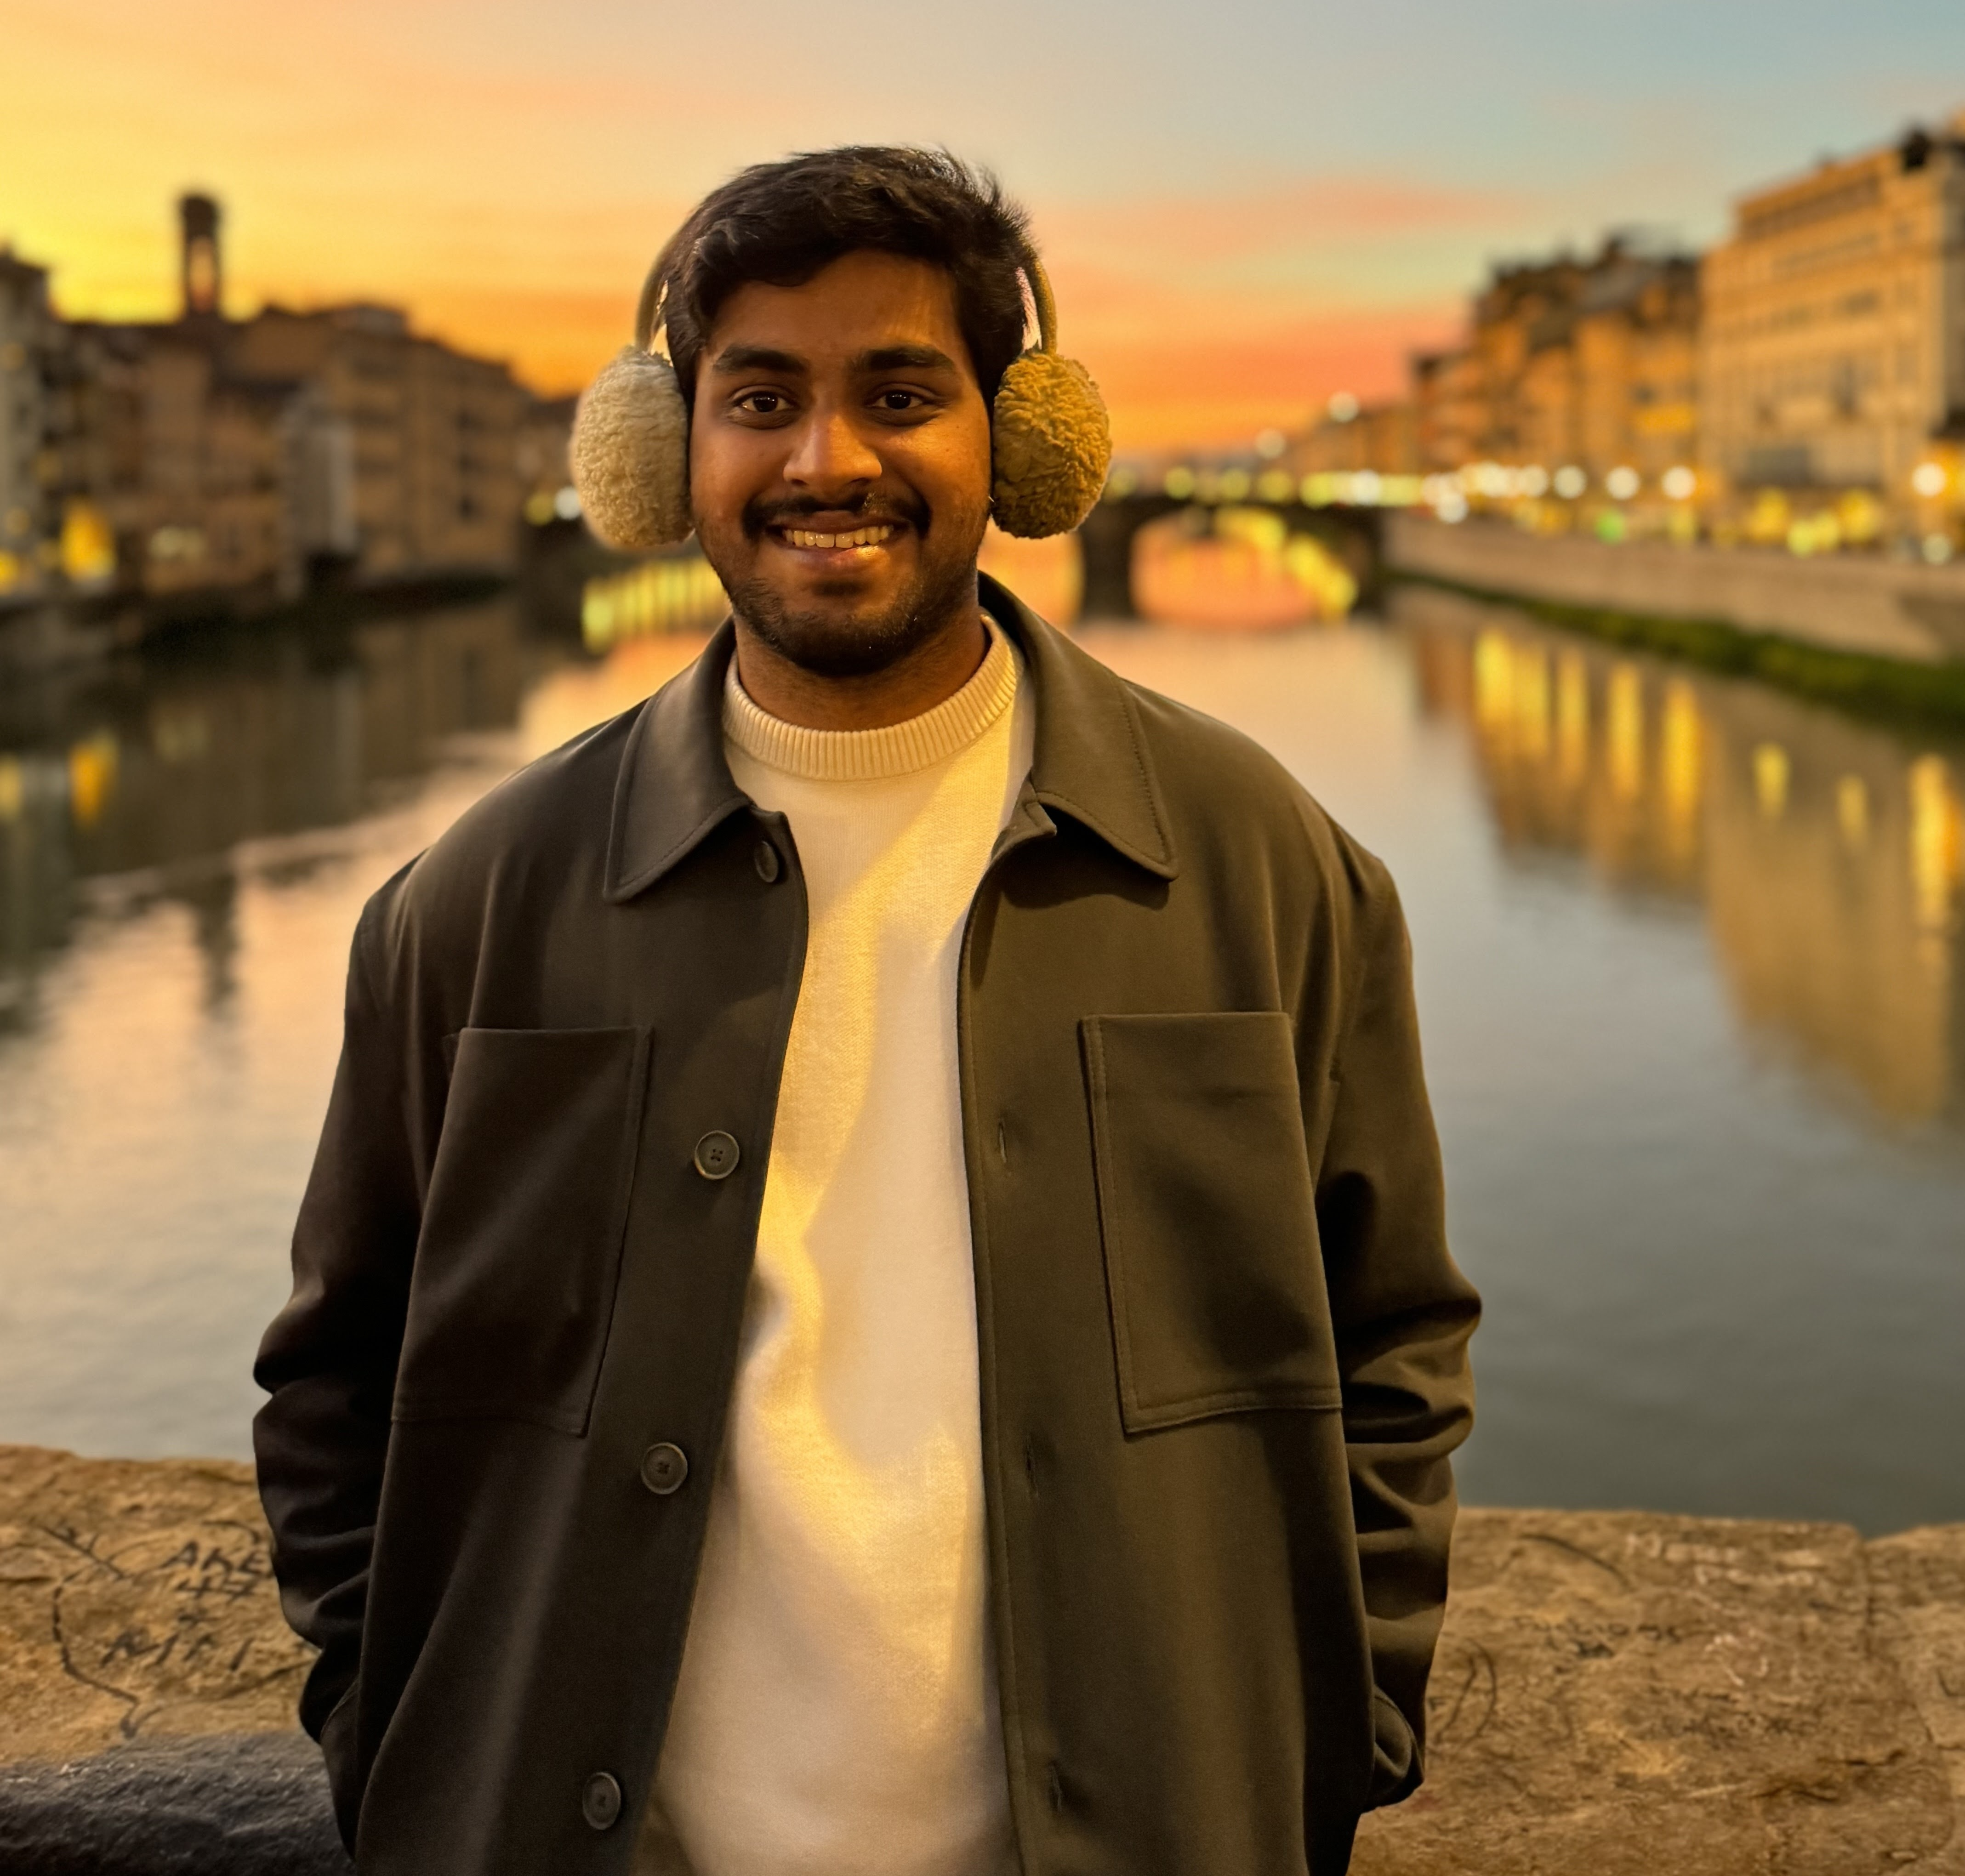
\includegraphics[height=1cm]{images/Shravan_Nayak.jpg}}
            %     \subfloat[]{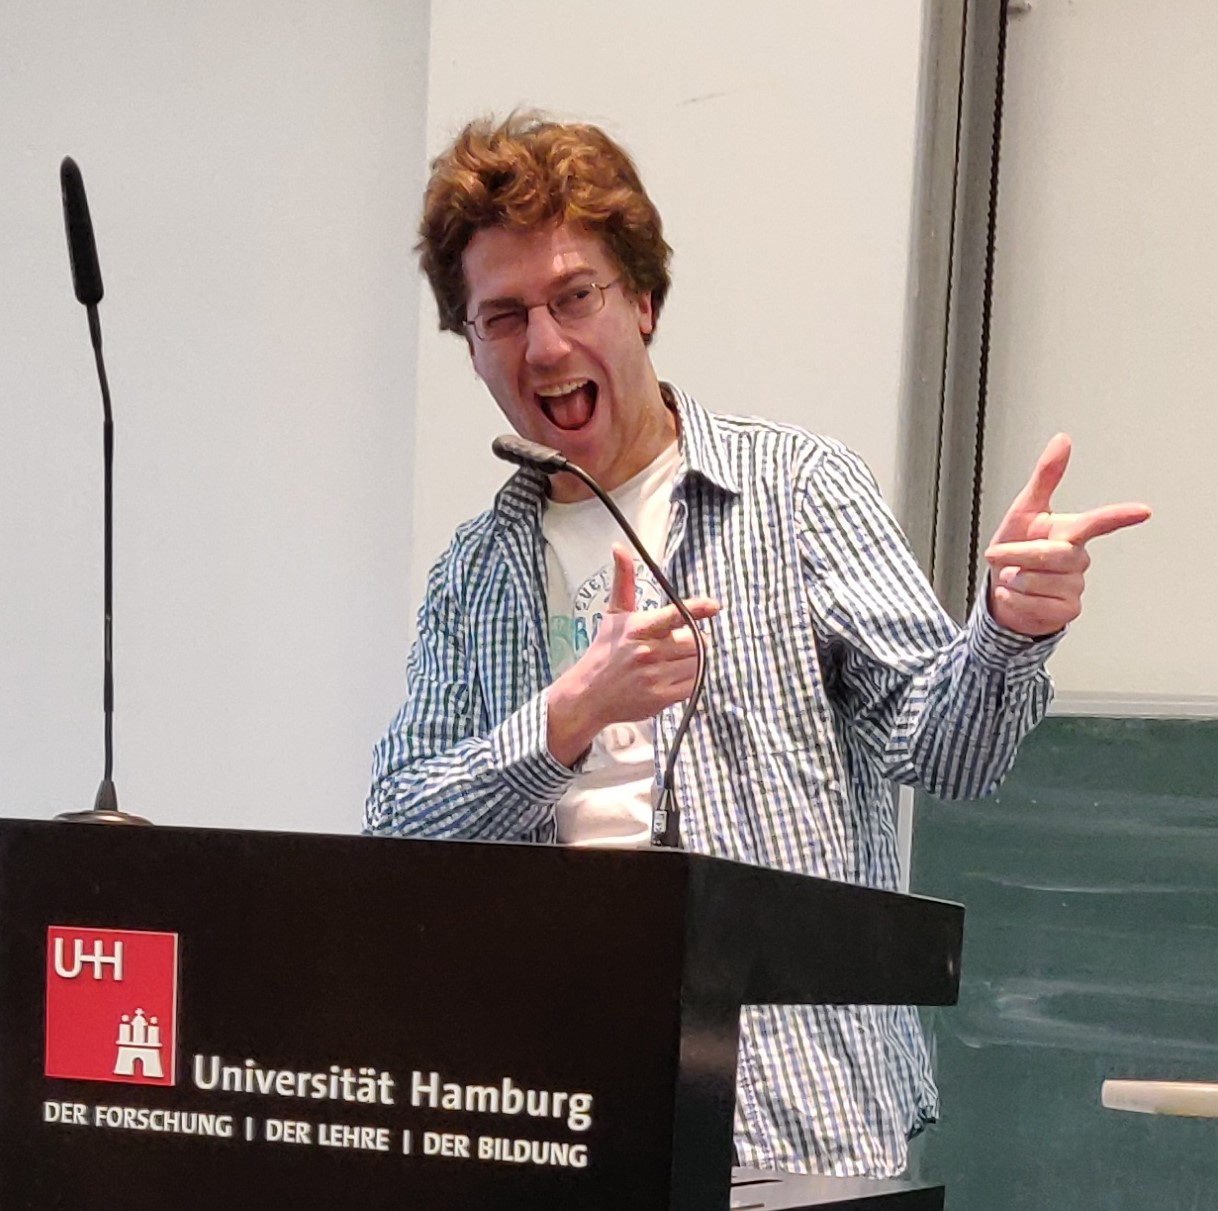
\includegraphics[height=1cm]{images/Christian_Schuler_Lecture.jpg}}
            %     \subfloat[]{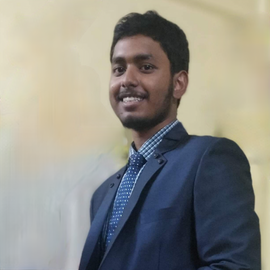
\includegraphics[height=1cm]{images/Debjoy_Saha.png}}
            %     \subfloat[]{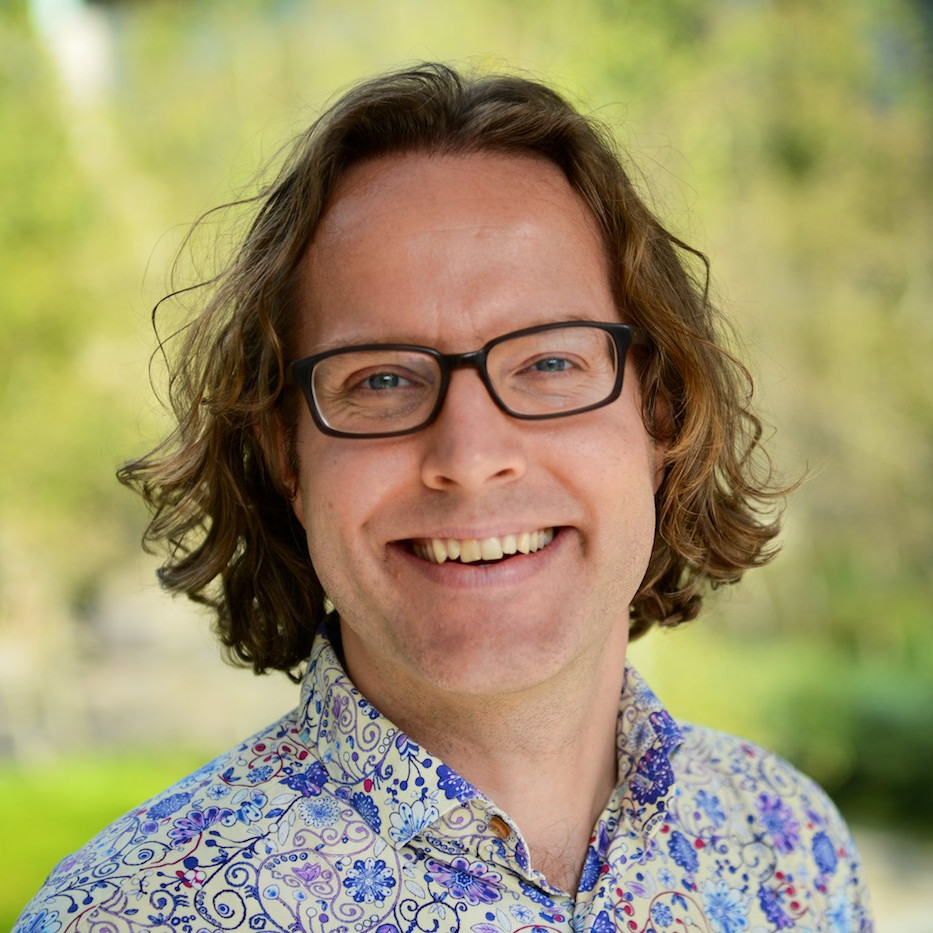
\includegraphics[height=1cm]{images/Timo_Baumann.jpg}}
            % \end{figure}
            %\\ Shravan, Christian, Debjoy, Timo
        \end{minipage}
    \end{minipage}

    \vspace{5mm}

    \begin{minipage}{1.0\textwidth}
        \begin{minipage}{.55\textwidth}
            \textbf{Linguistic information in pauses}
            \par\noindent\rule{\textwidth}{0.4pt}
            {\color{thiscolor}$\bullet$} Can We See Your Response Before You Speak? Exploring Linguistic Information Found in Inter-Utterance Pauses 
            \\ \citep{schuler2024CanWeSee}
            %\vspace{-10mm}
        \end{minipage}
        \begin{minipage}{.44\textwidth}
            \centering
            \begin{minipage}{.24\textwidth}
                \centering
                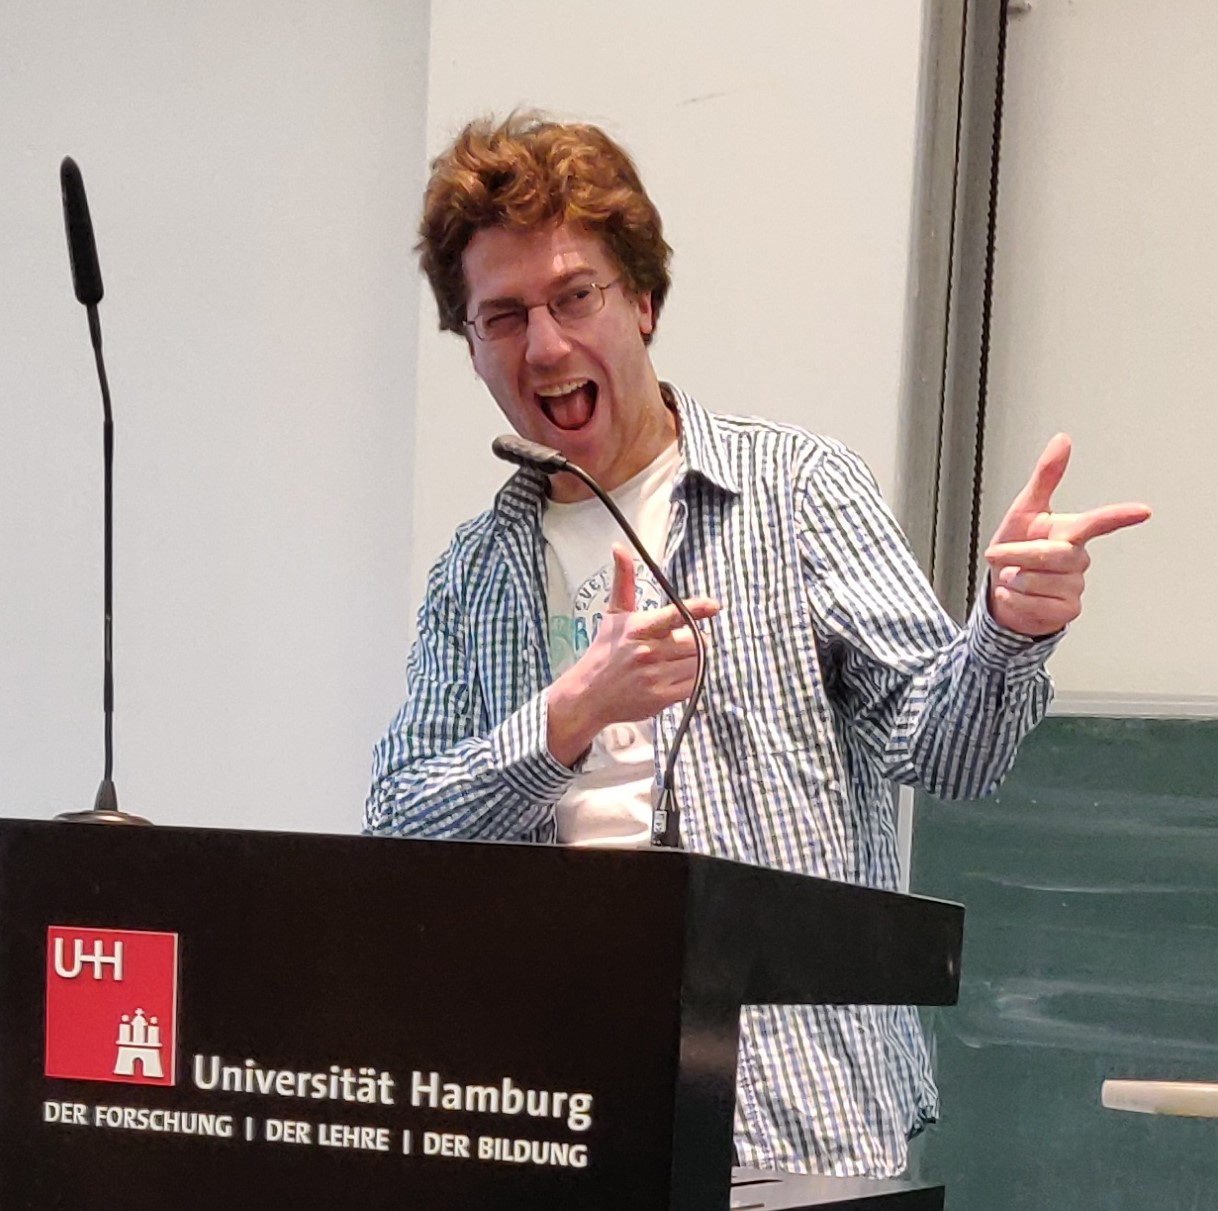
\includegraphics[height=1.4cm]{images/Christian_Schuler_Lecture.jpg} 
                Christian
            \end{minipage}%
            \begin{minipage}{.24\textwidth}
                \centering
                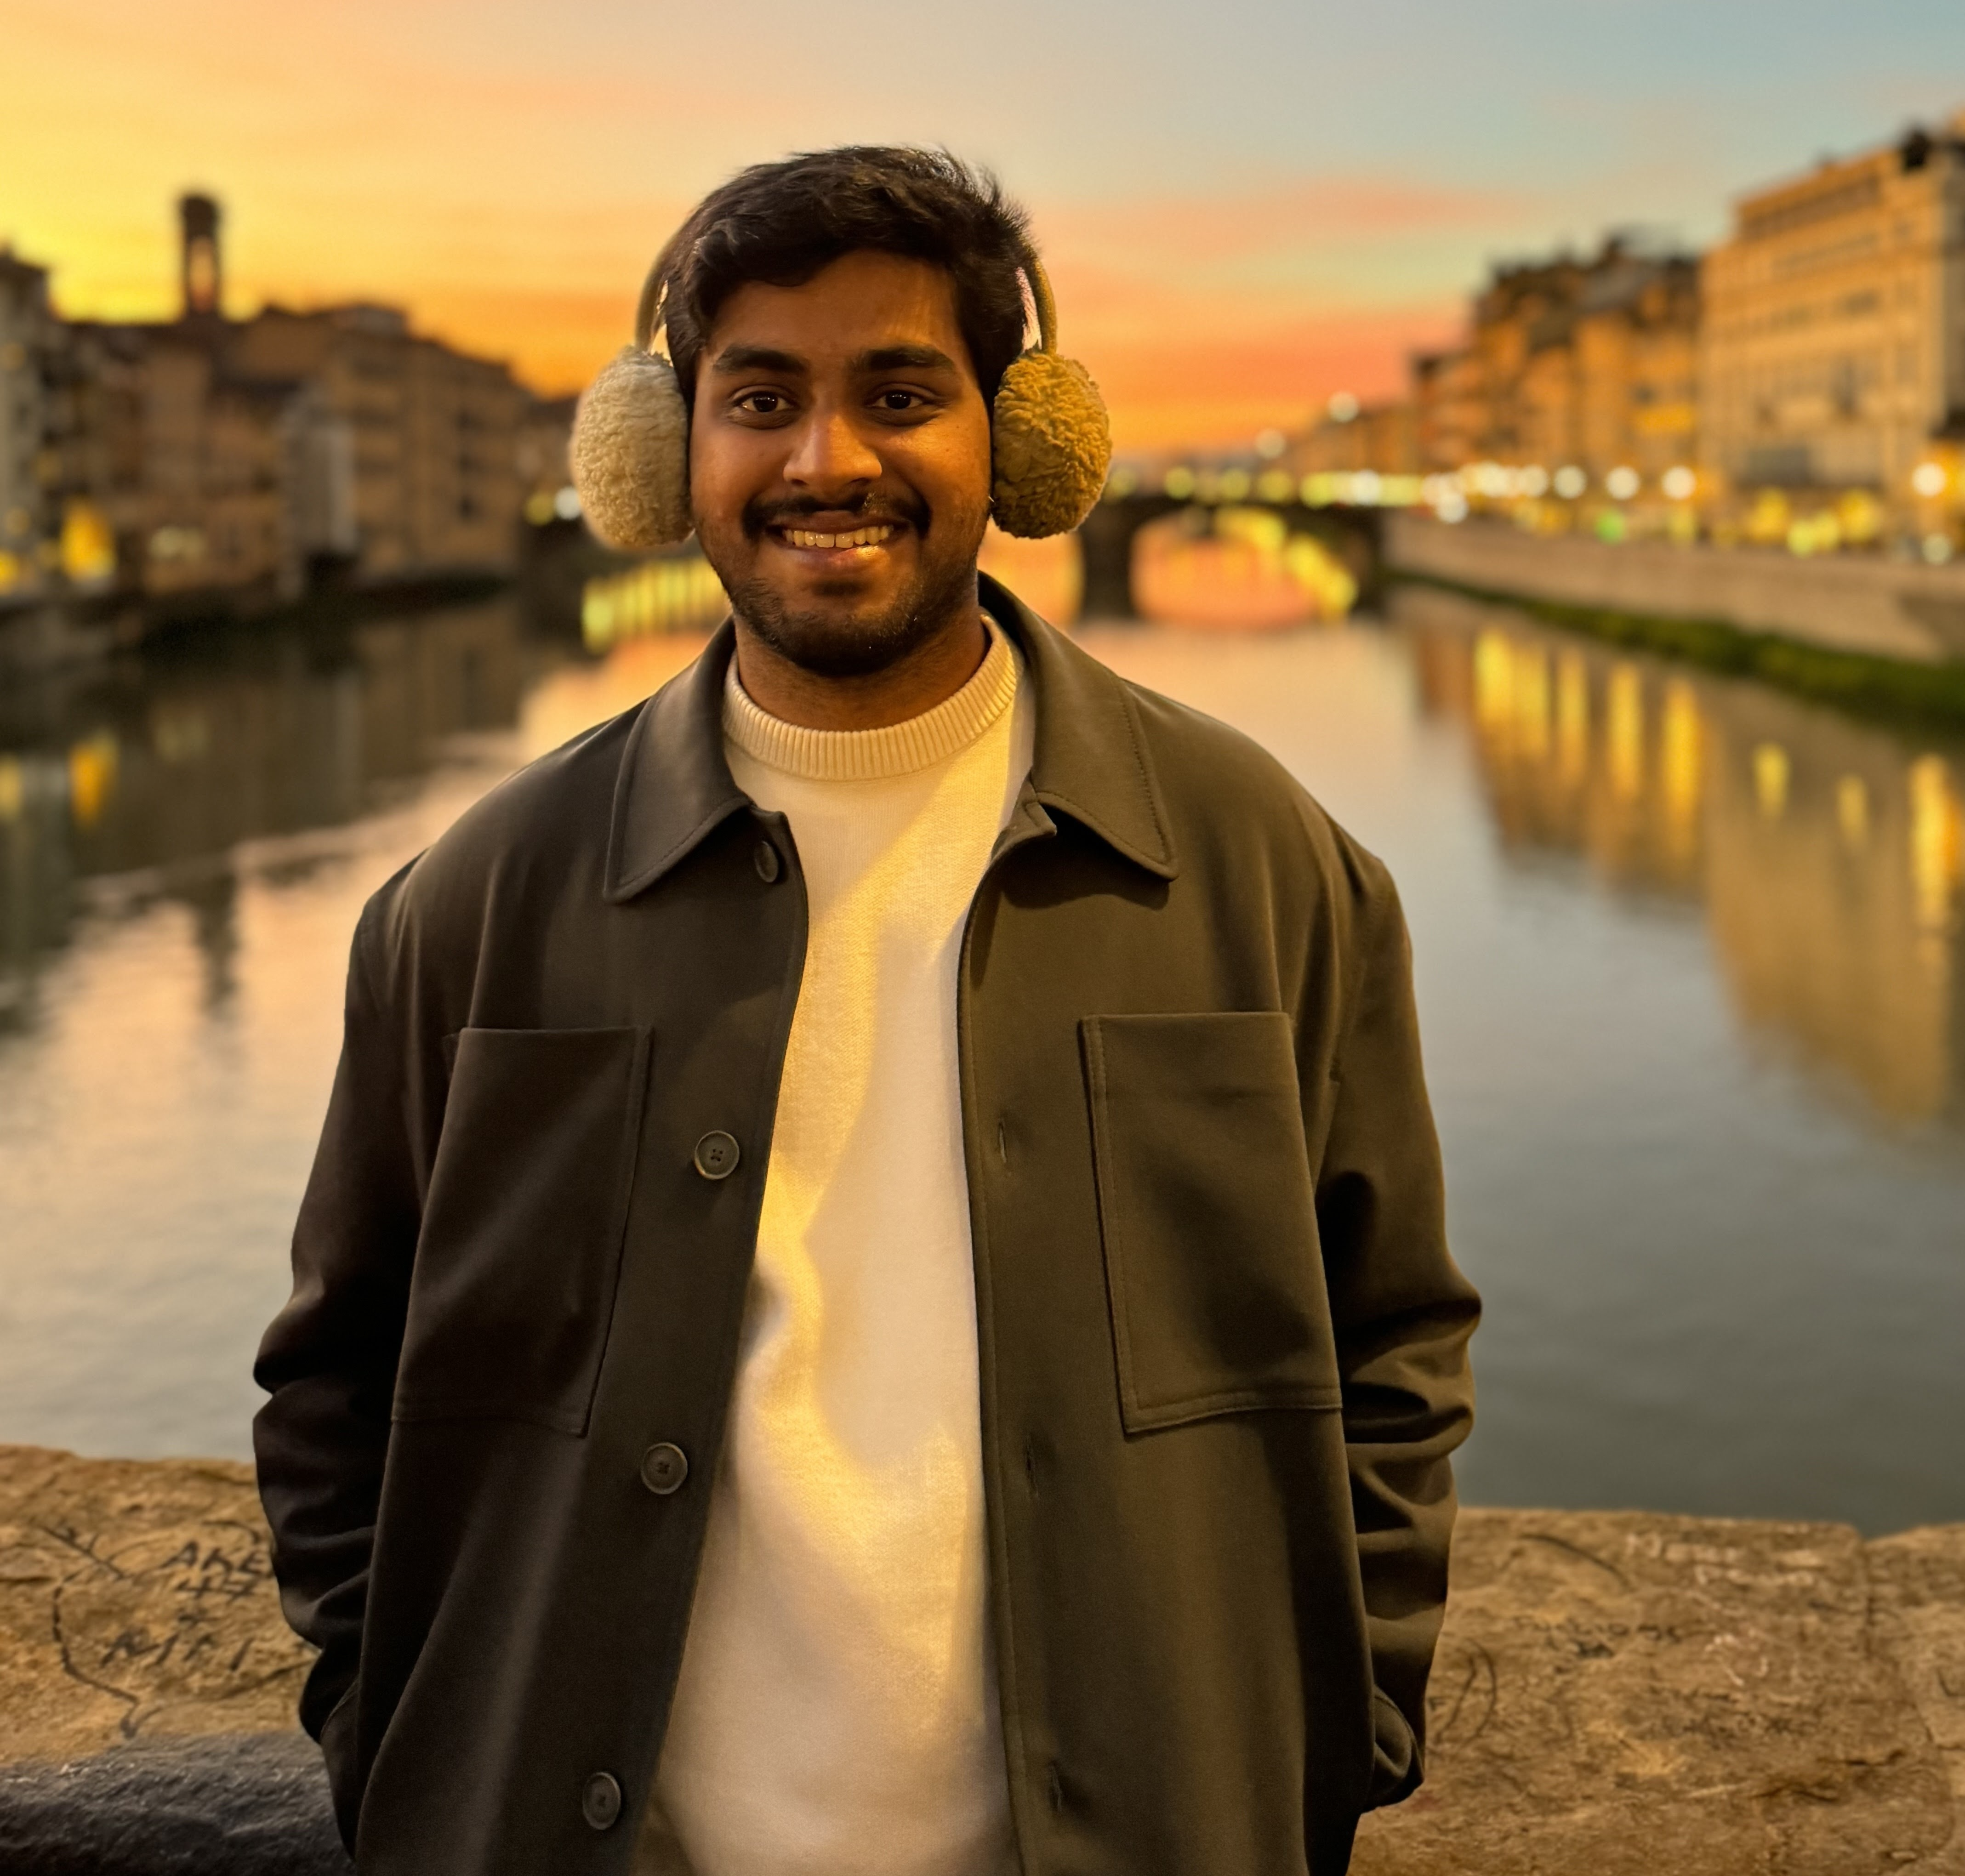
\includegraphics[height=1.4cm]{images/Shravan_Nayak.jpg}
                Shravan
            \end{minipage}%
            \begin{minipage}{.24\textwidth}
                \centering
                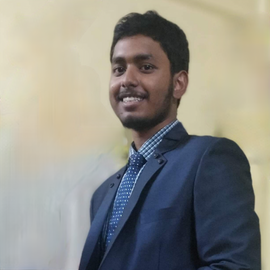
\includegraphics[height=1.4cm]{images/Debjoy_Saha.png}
                Debjoy
            \end{minipage}%
            \begin{minipage}{.24\textwidth}
                \centering
                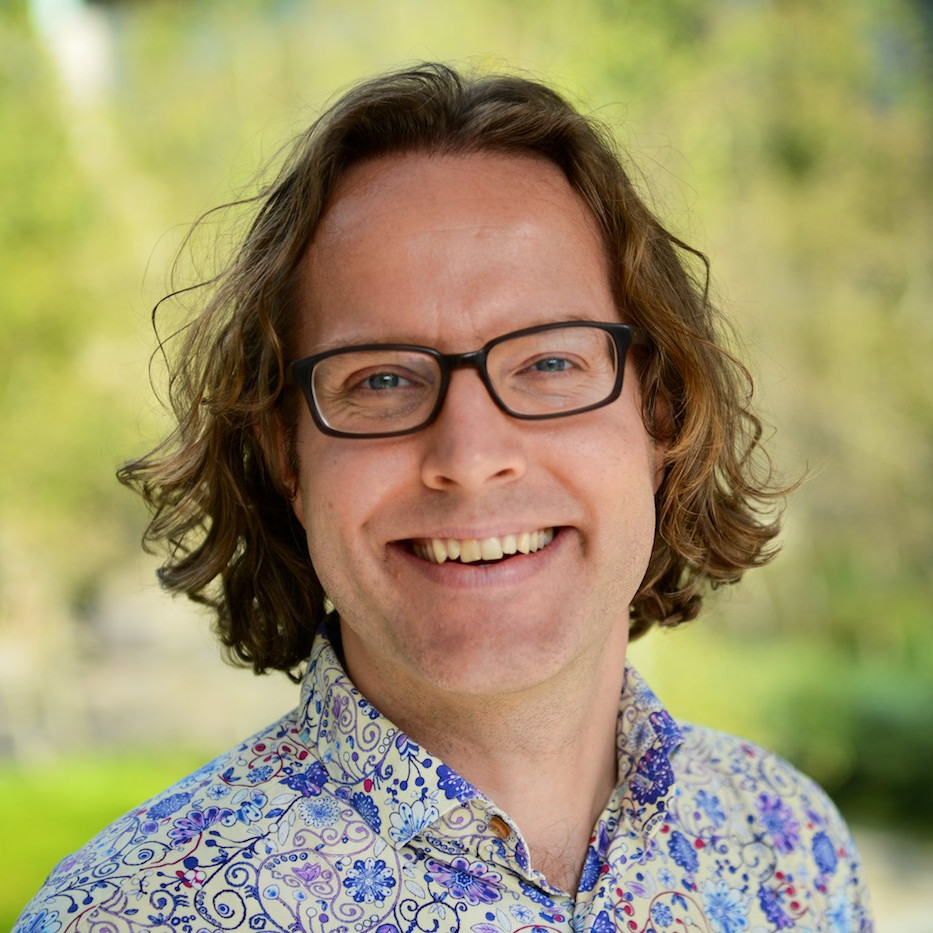
\includegraphics[height=1.4cm]{images/Timo_Baumann.jpg}
                Timo
            \end{minipage}
            % \begin{figure}
            % \centering
            % \captionsetup[subfigure]{labelformat=empty}
            %     \subfloat[]{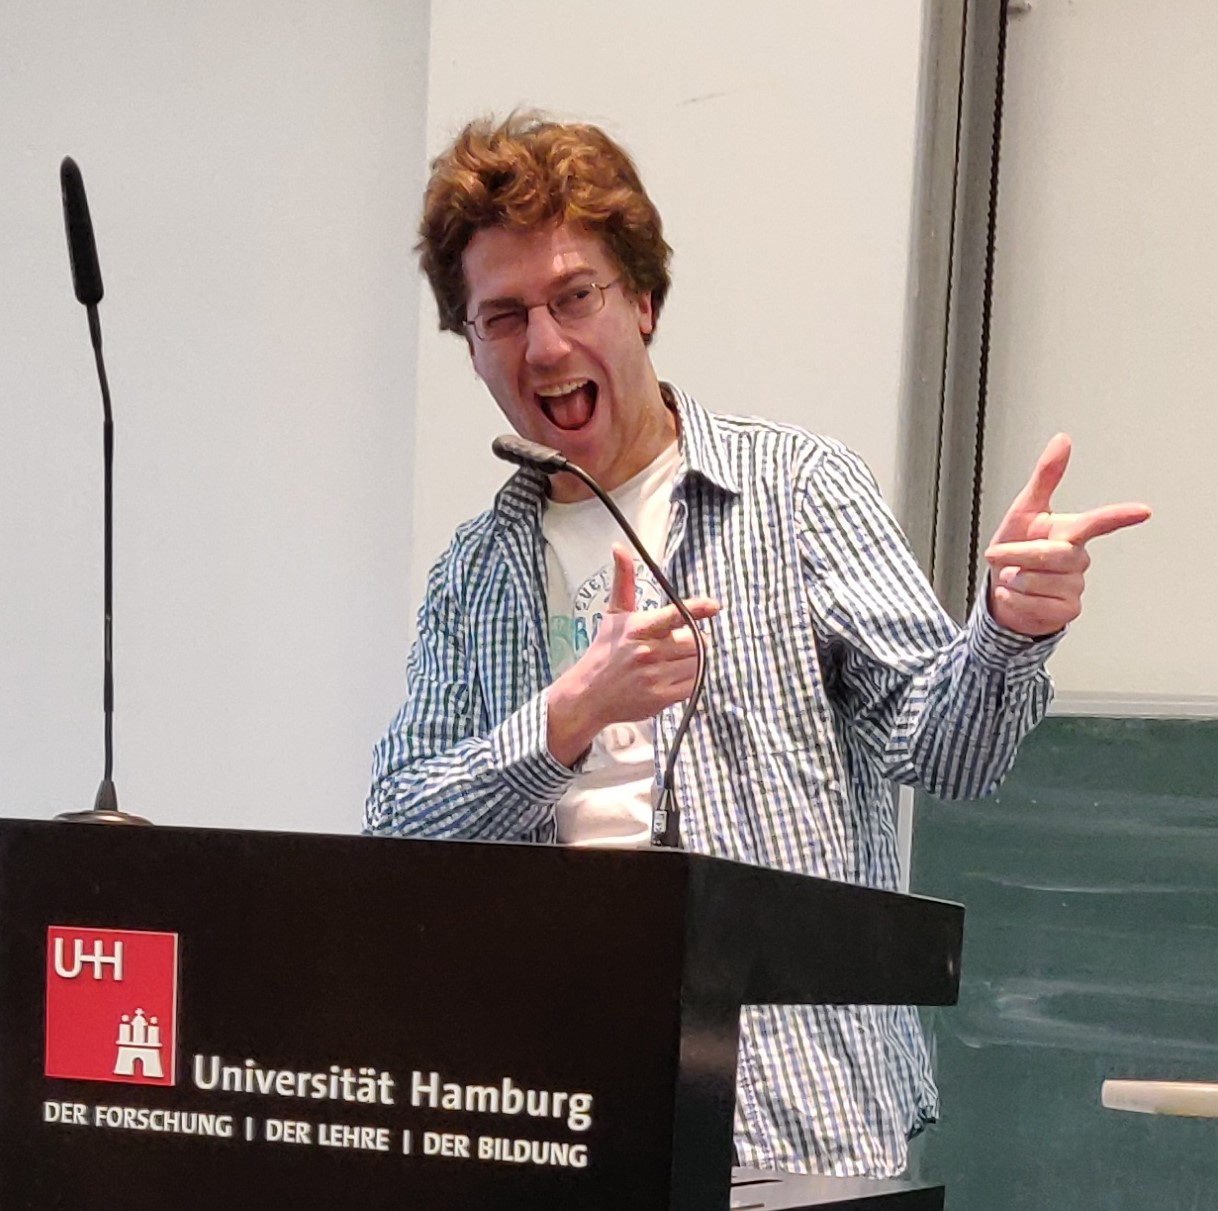
\includegraphics[height=1cm]{images/Christian_Schuler_Lecture.jpg}}
            %     \subfloat[]{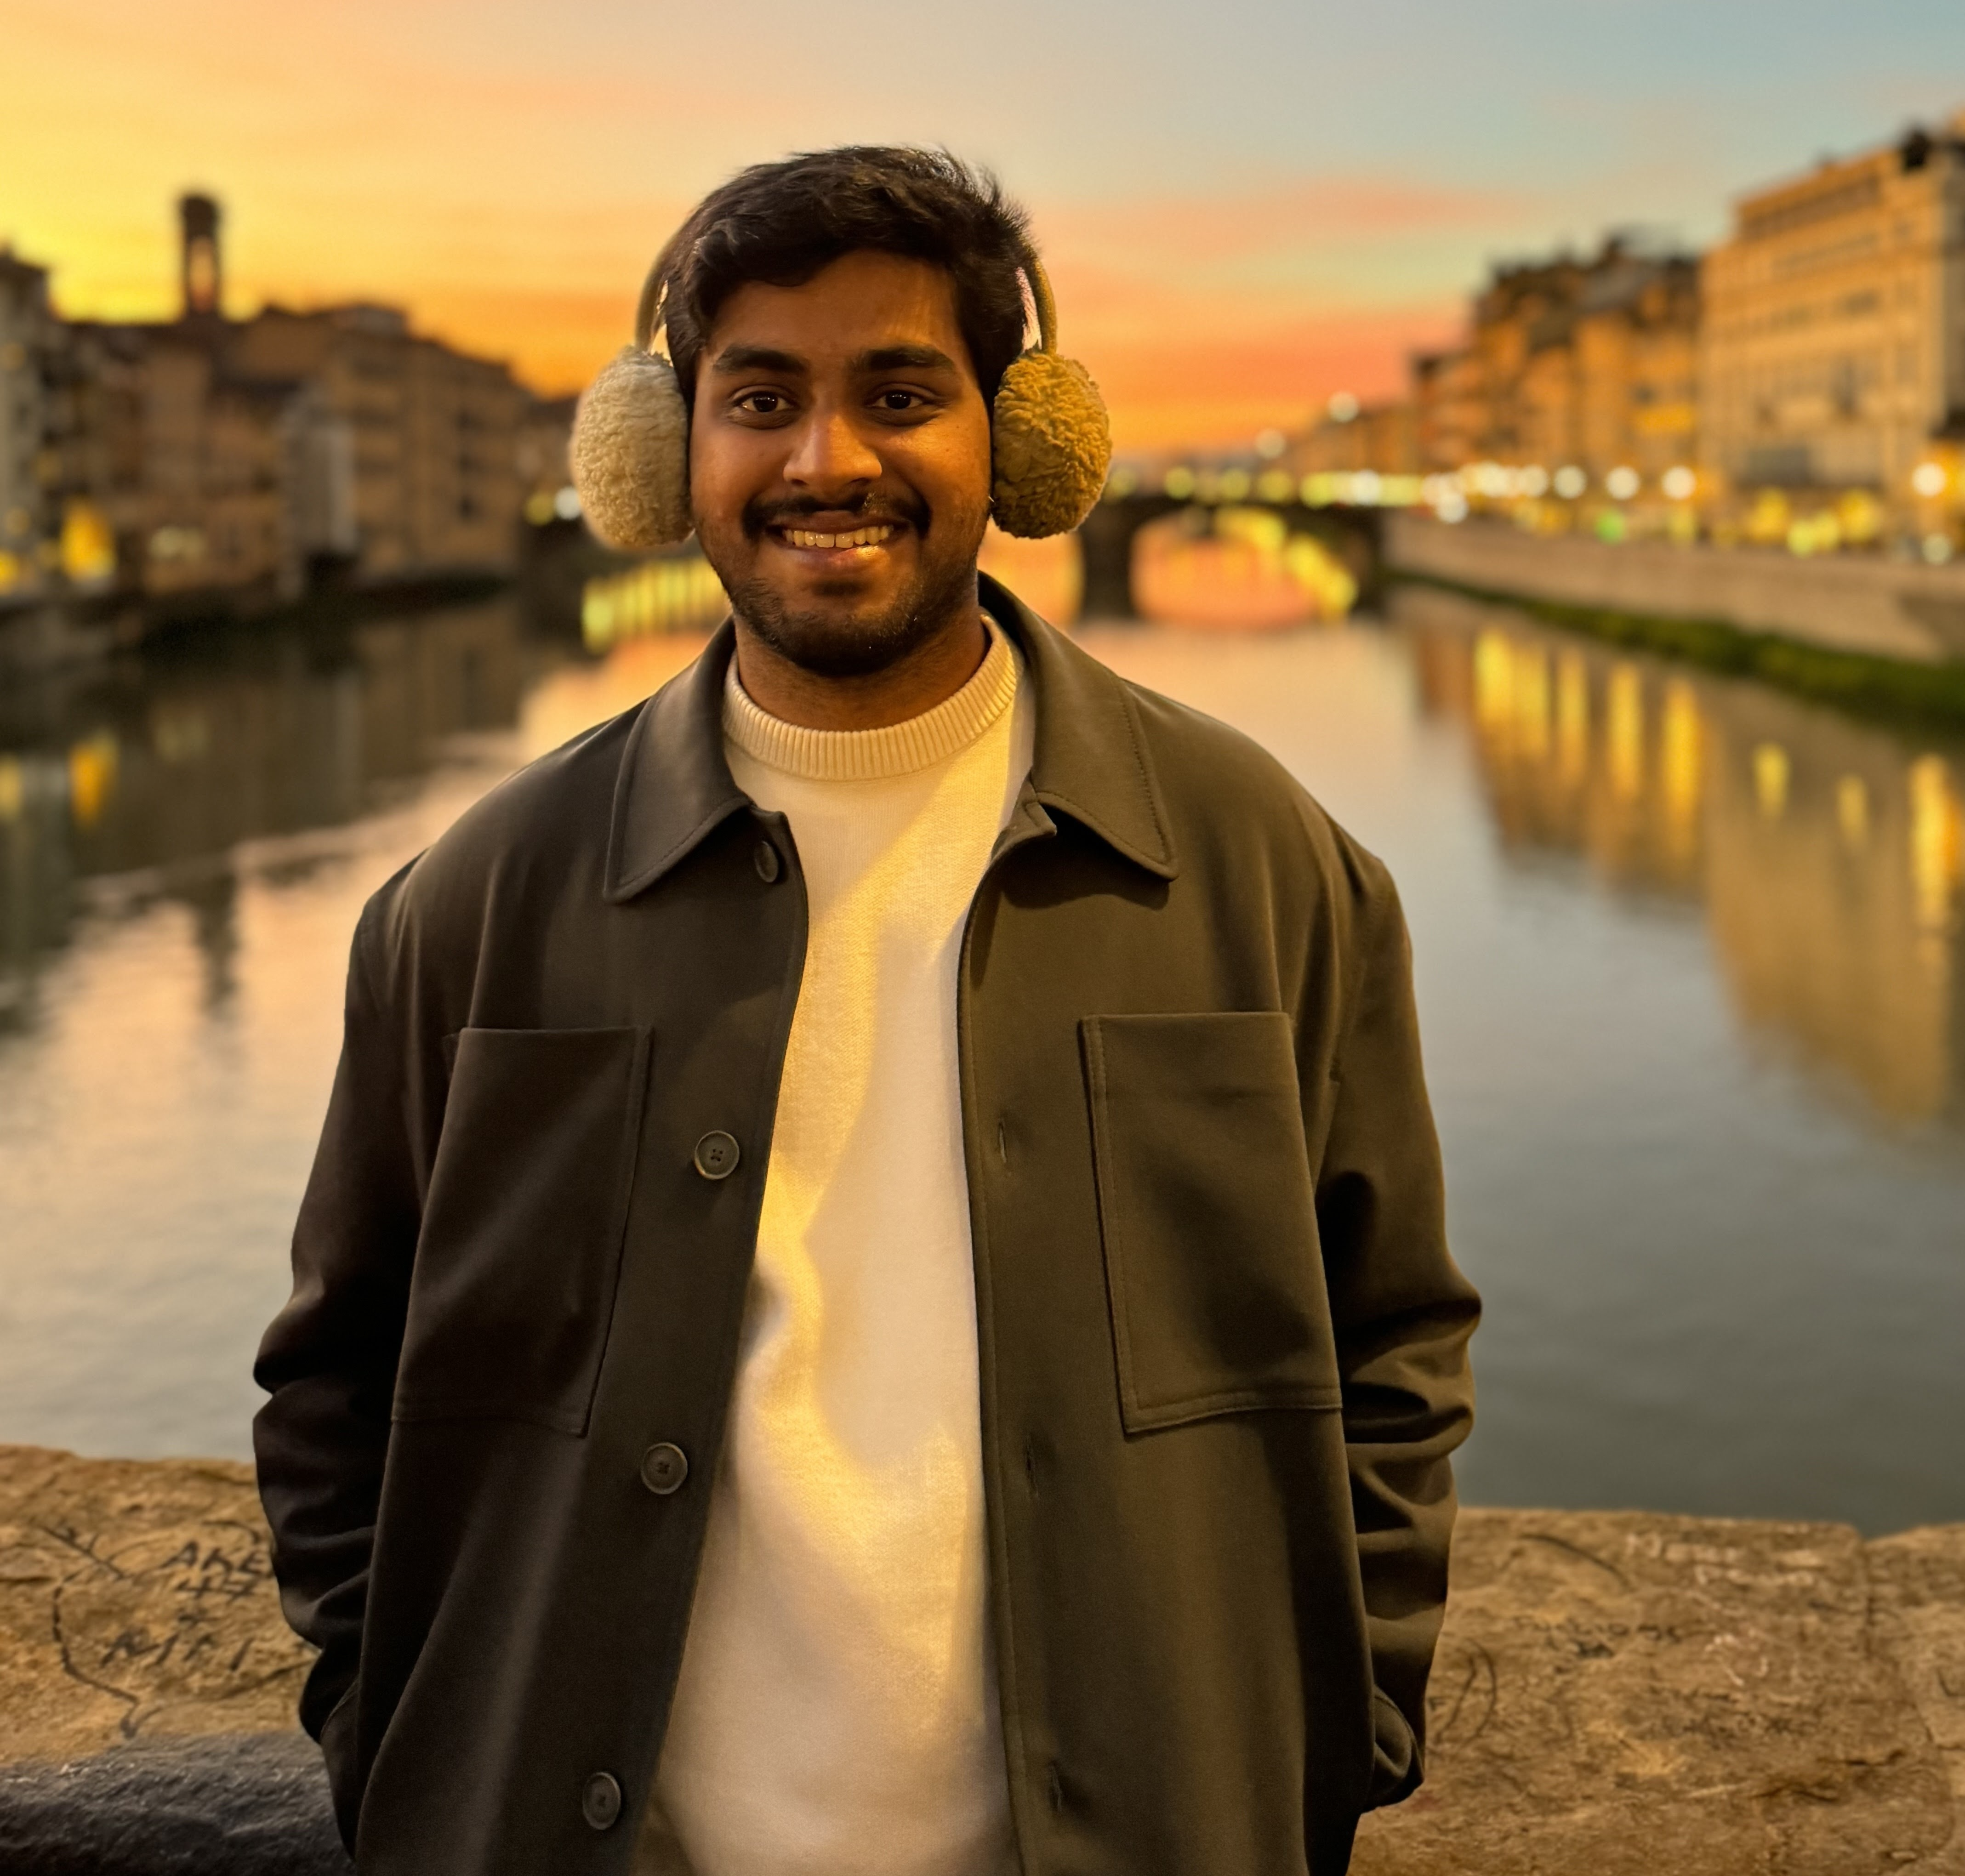
\includegraphics[height=1cm]{images/Shravan_Nayak.jpg}}
            %     \subfloat[]{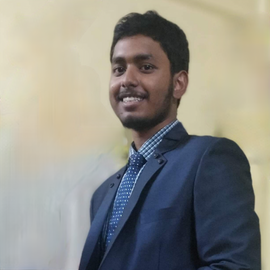
\includegraphics[height=1cm]{images/Debjoy_Saha.png}}
            %     \subfloat[]{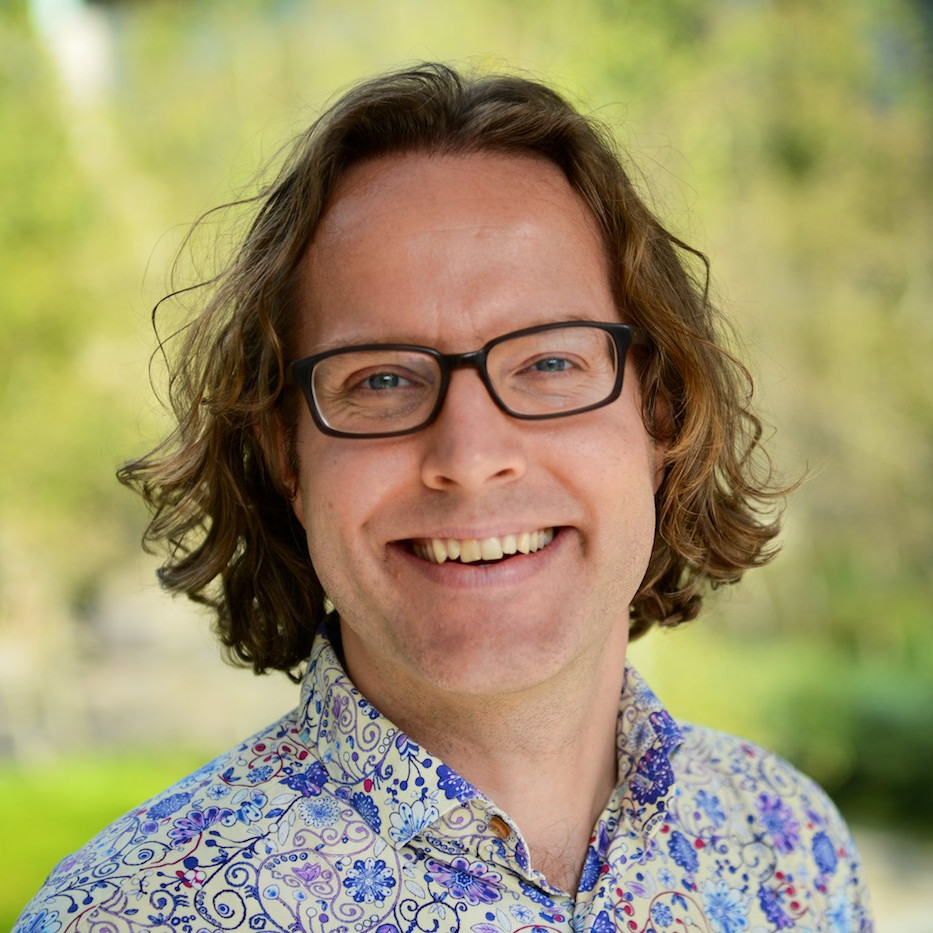
\includegraphics[height=1cm]{images/Timo_Baumann.jpg}}
            % \end{figure}
            %\\ Christian, Shravan, Debjoy, Timo
        \end{minipage}
    \end{minipage}
\end{frame}

% #############################################################################
\section{Master}

\begin{frame}[fragile]
	\frametitle{Master's Thesis Build-up I}
    \begin{minipage}{.49\textwidth}
        {\color{thiscolor}$\bullet$} Towards a Complete Mapping \\ of Kurdish Dialectology 
        \\ \citep{schuler2023CompleteMappingKurdish} Poster as ICKL6
        \vspace{5mm}
        \begin{minipage}{.70\textwidth}
            \centering
            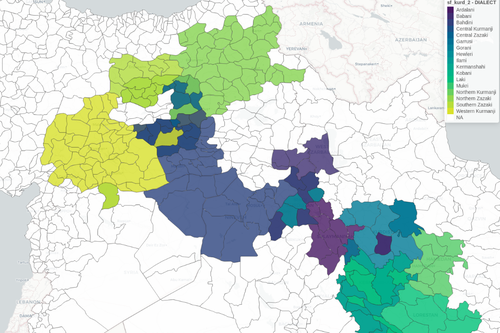
\includegraphics[width=\textwidth]{images/ickl6_dialectmapping.png}
        \end{minipage}%
        \begin{minipage}{.30\textwidth}
            \centering
            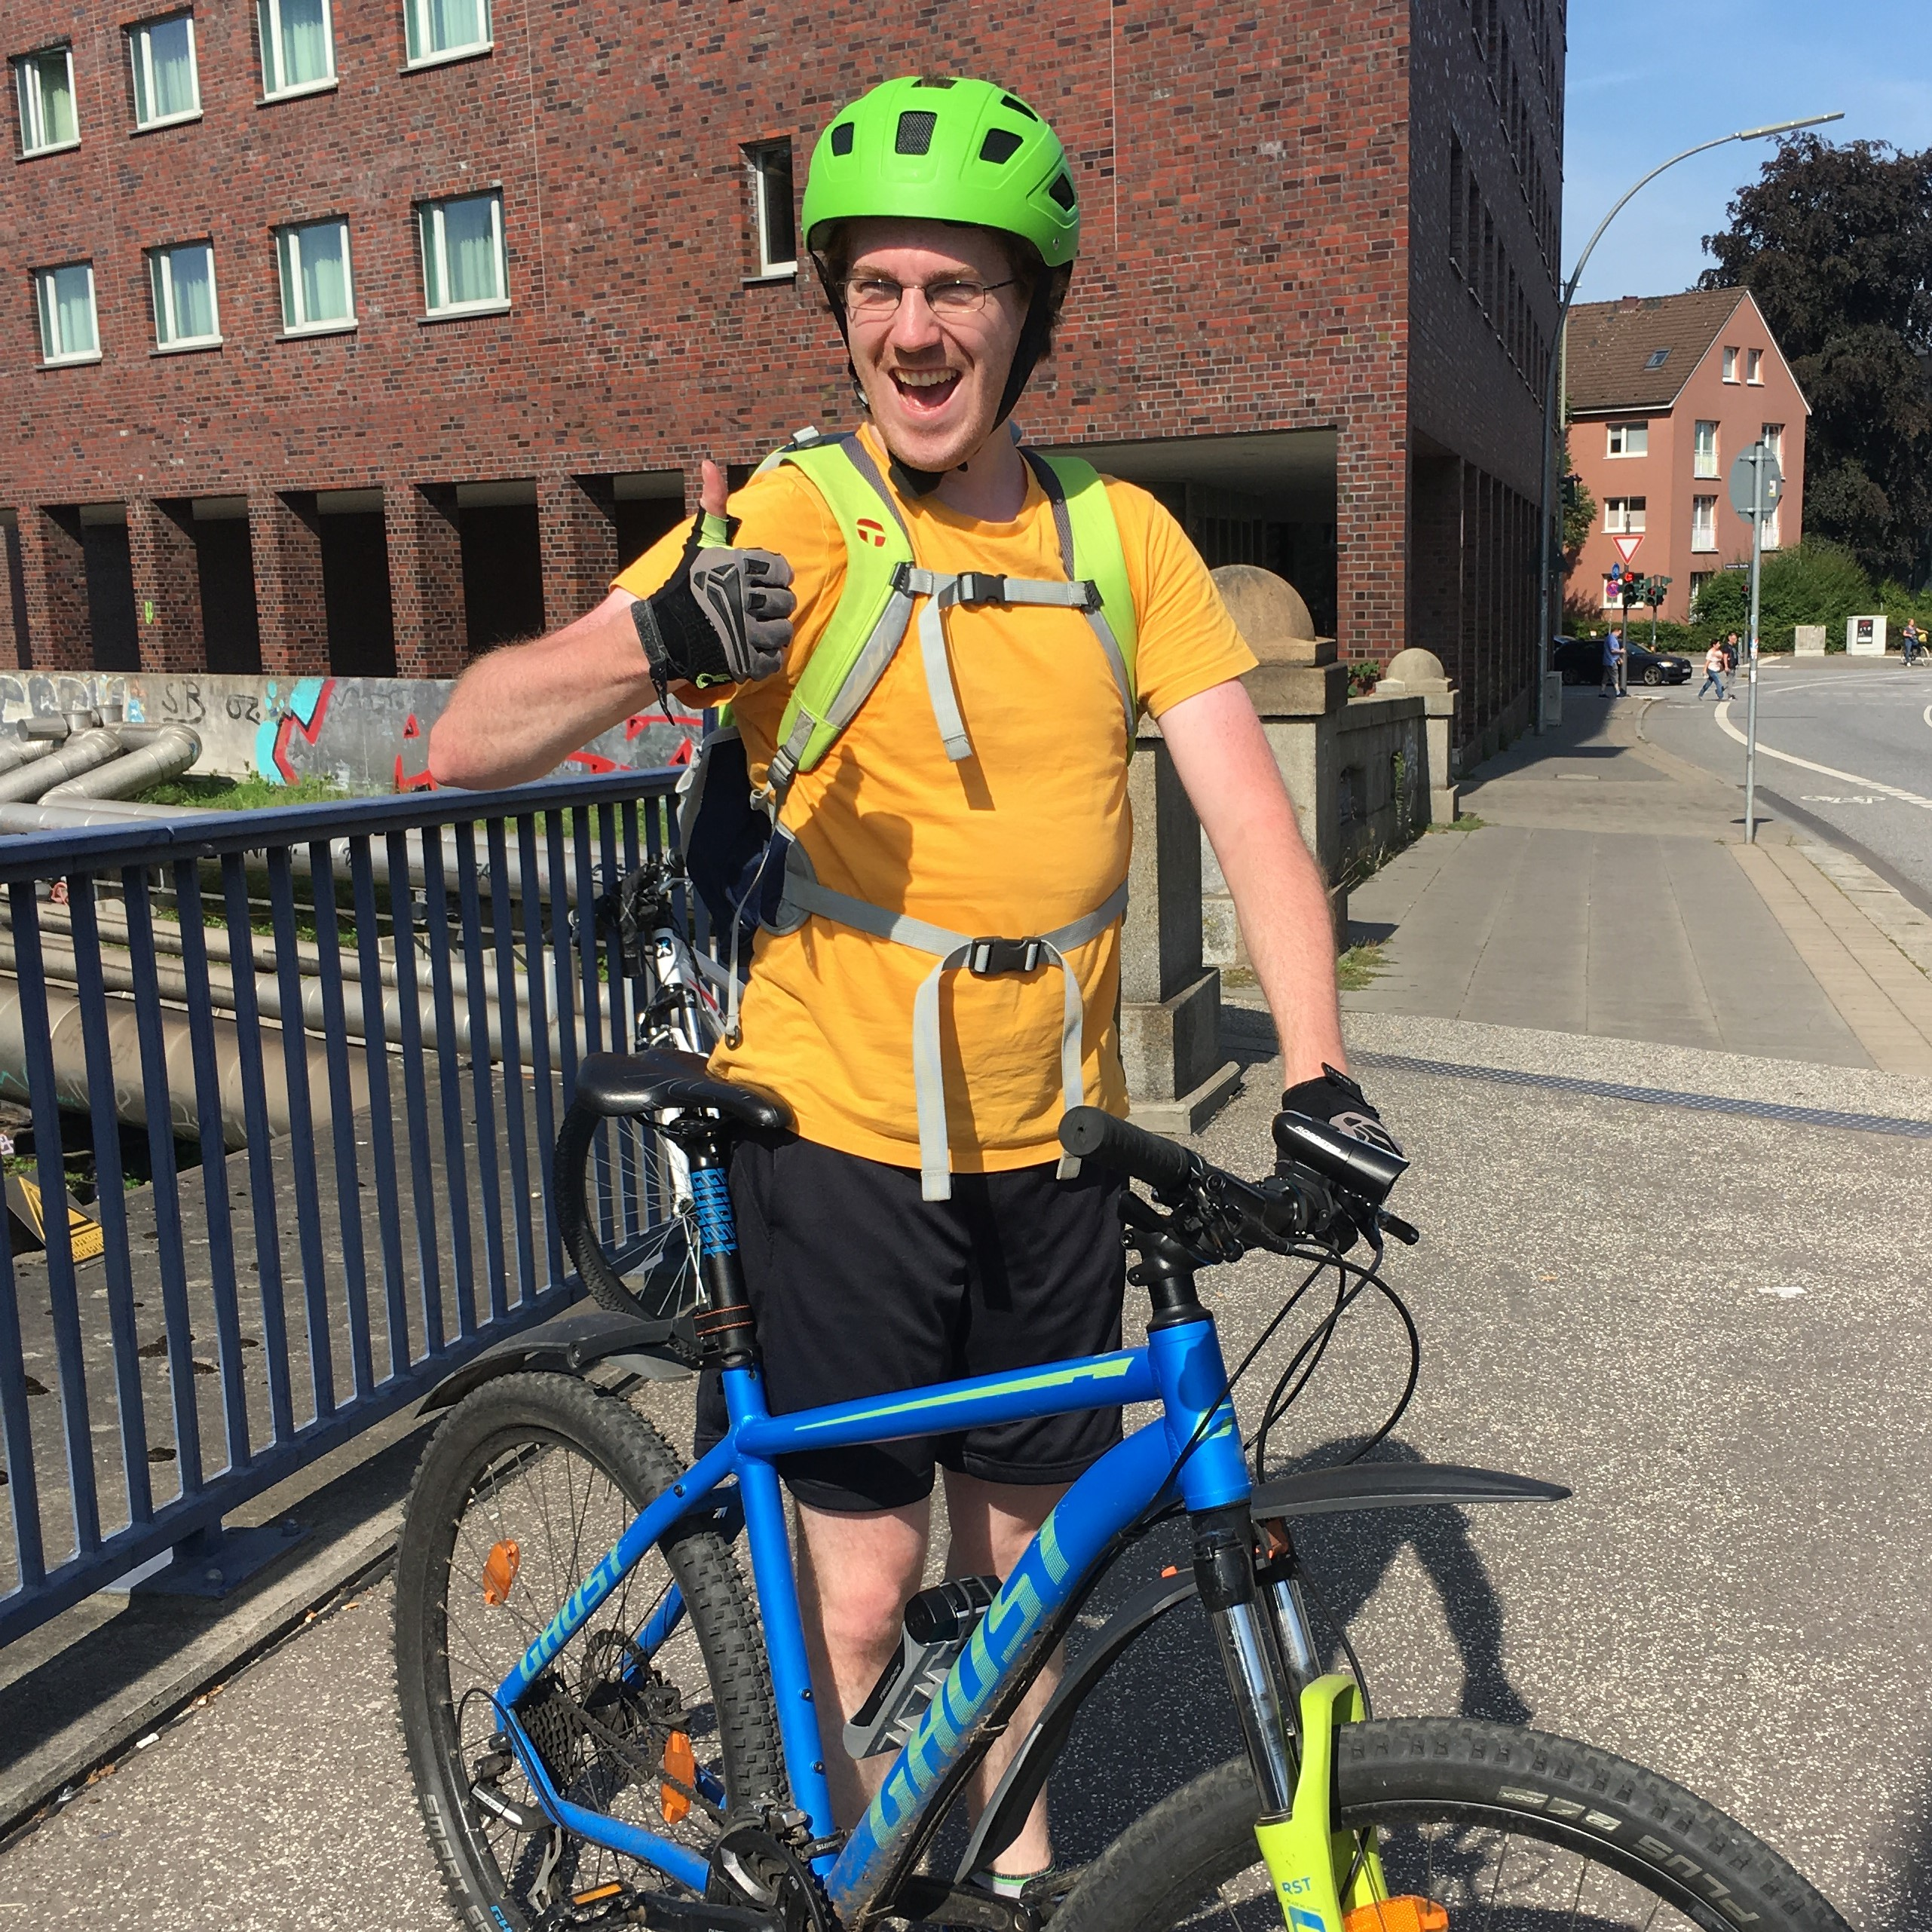
\includegraphics[height=1.3cm]{images/Christian_Schuler_Bike.JPG}
            %\\ 
            Christian
            \vspace{0.5cm}
            \\ 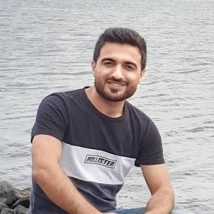
\includegraphics[height=1.3cm]{images/Raman_Ahmad.png} 
            %\\ 
            Raman
        \end{minipage}
        % 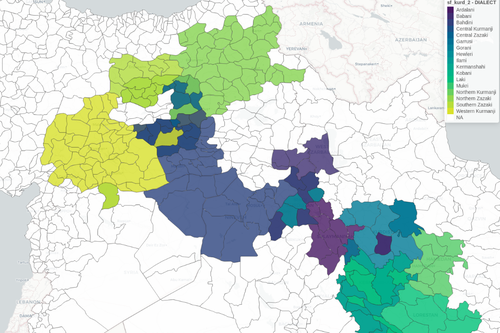
\includegraphics[height=2.5cm]{images/ickl6_dialectmapping.png}
        % 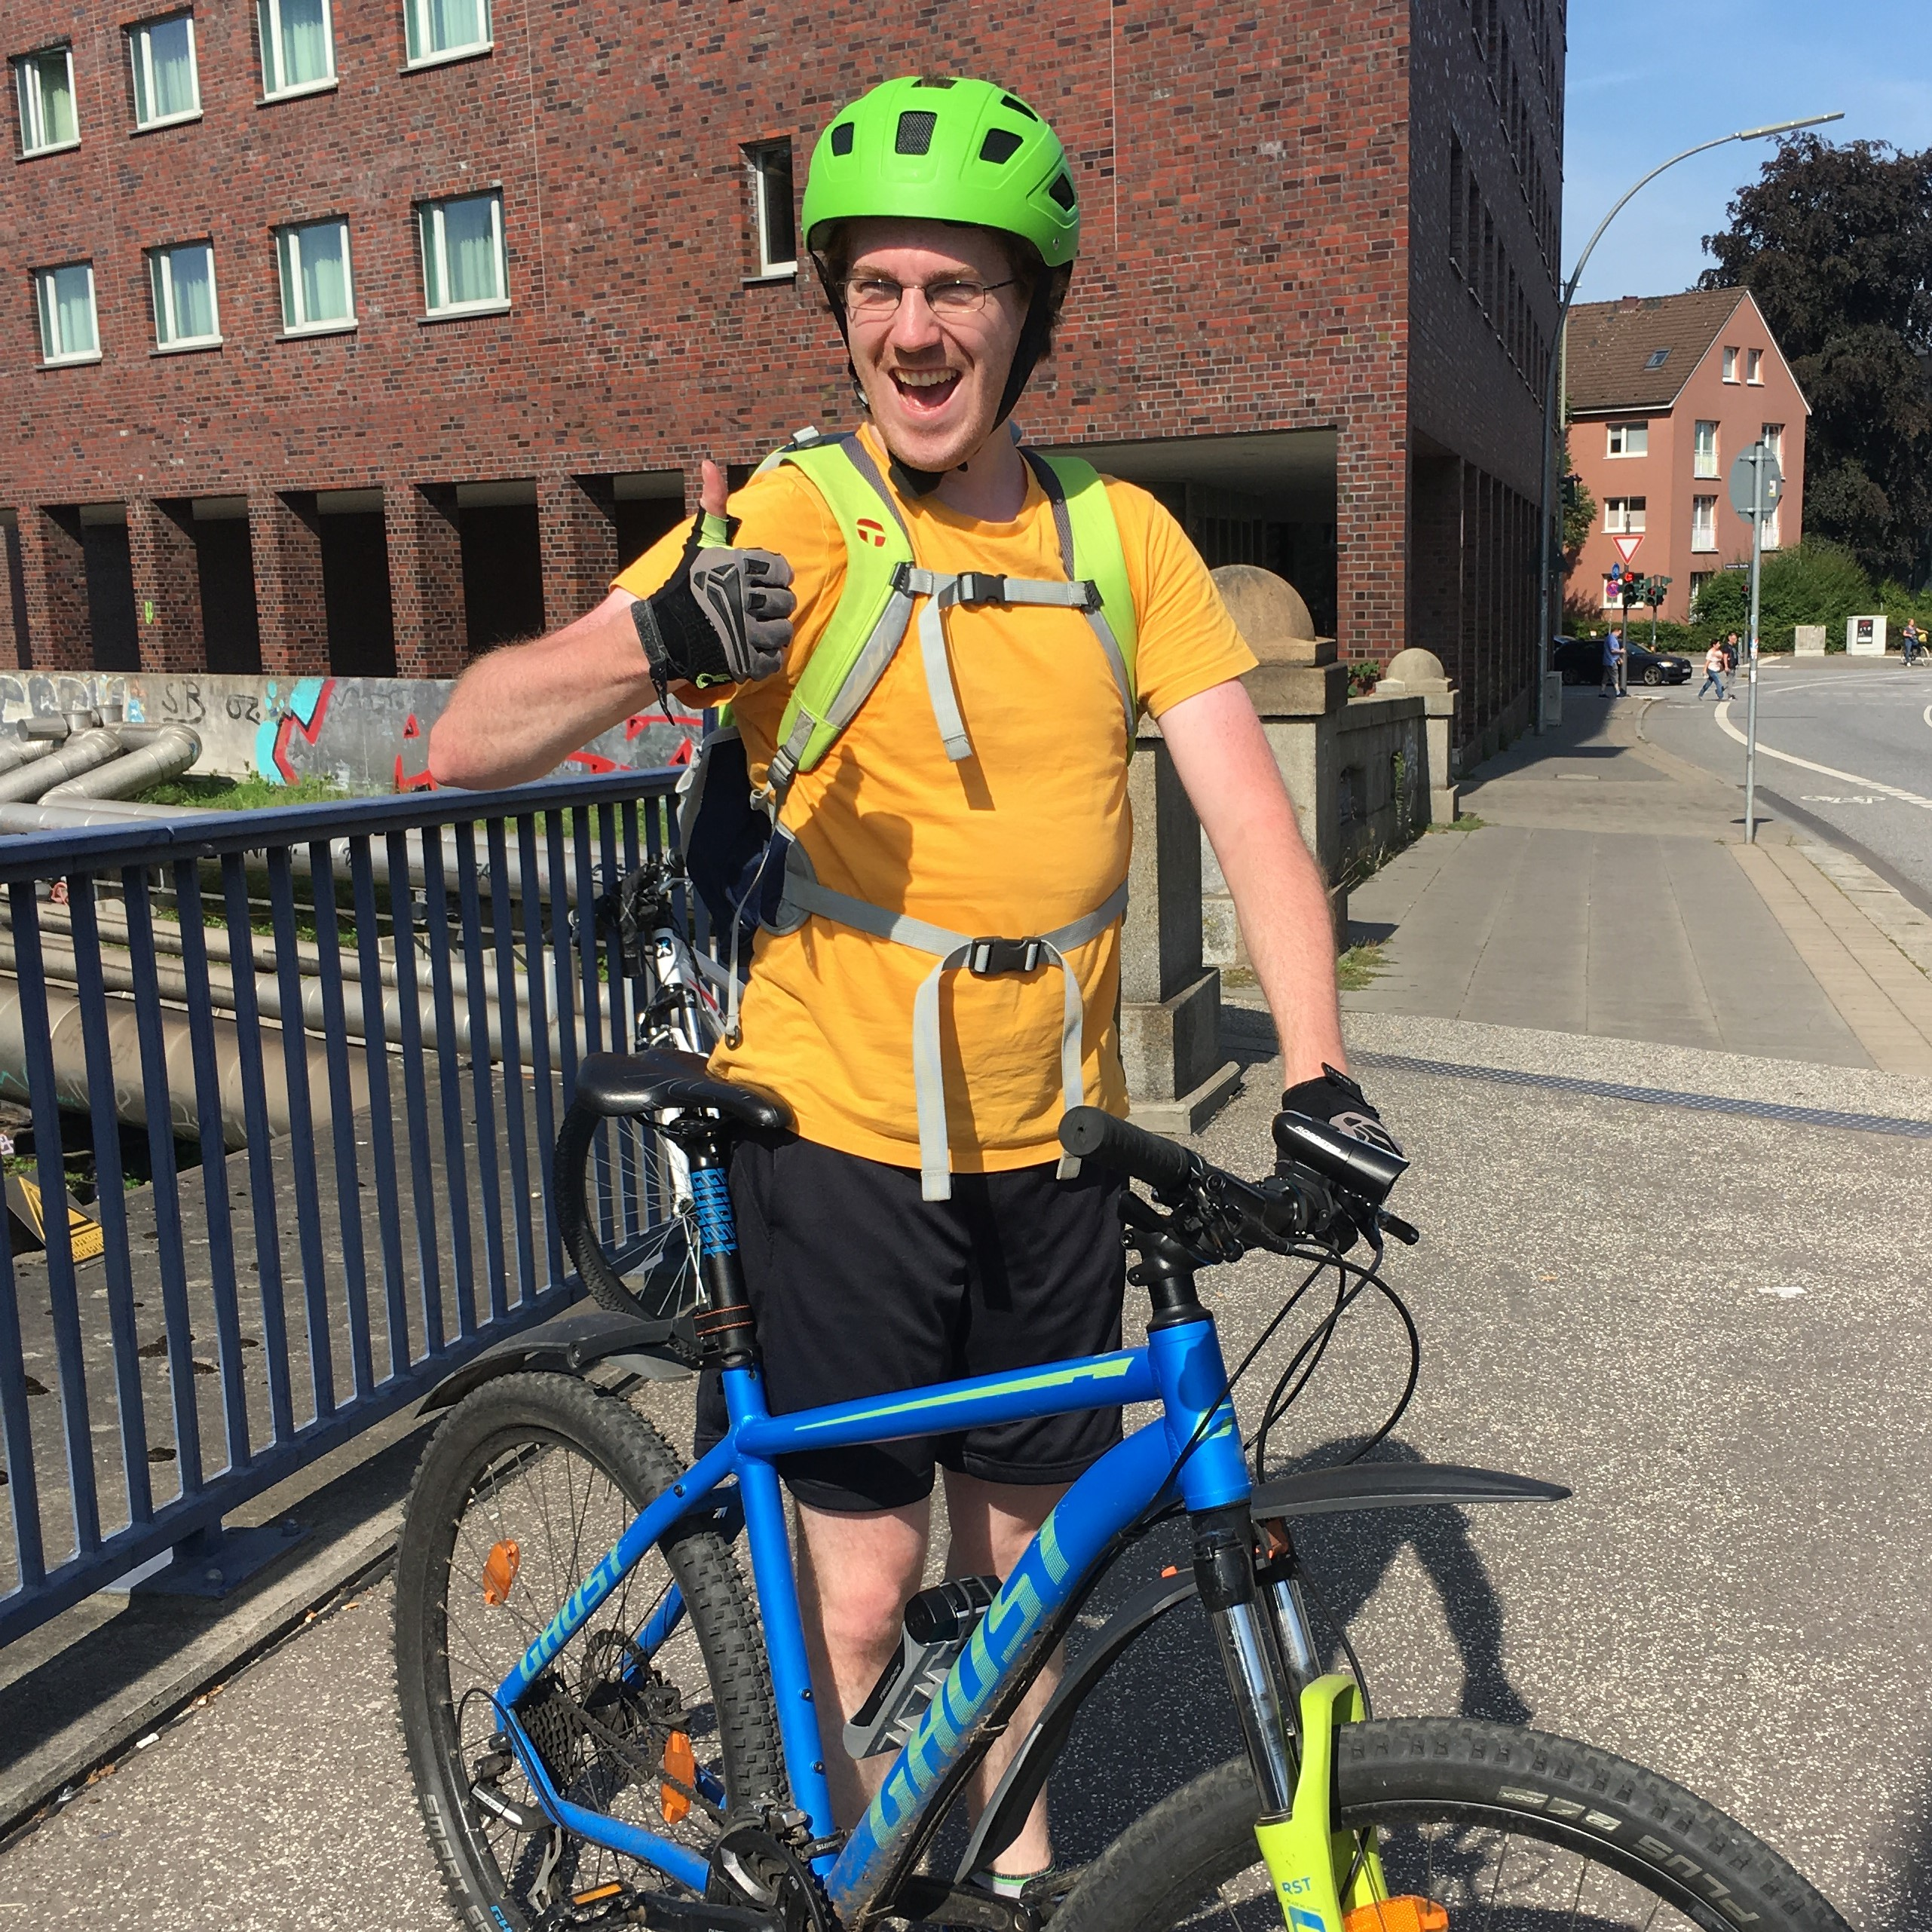
\includegraphics[height=1.2cm]{images/Christian_Schuler_Bike.JPG} 
        % 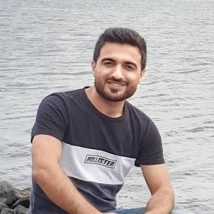
\includegraphics[height=1.2cm]{images/Raman_Ahmad.png} 
    \end{minipage}\hfill%
    \begin{minipage}{.49\textwidth}
        {\color{thiscolor}$\bullet$} Analysis of Phonology and Morphology \\ in the Kobani Dialect 
        \\ \citep{ahmad2023AnalysisPhonologyMorphology} Poster as ICKL6
        \vspace{5mm}
        \begin{minipage}{.70\textwidth}
            \centering
            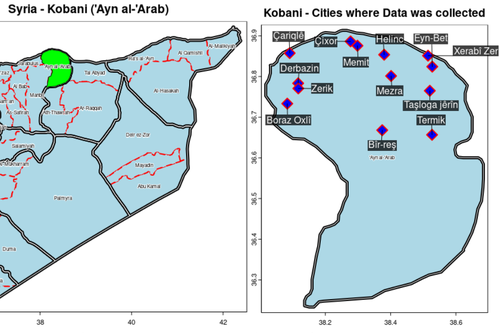
\includegraphics[width=\textwidth]{images/ickl6_kobanianalysis.png}
        \end{minipage}%
        \begin{minipage}{.30\textwidth}
            \centering
            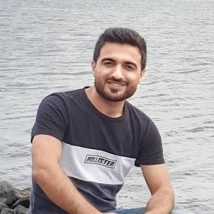
\includegraphics[height=1.3cm]{images/Raman_Ahmad.png}
            %\\ 
            Raman
            \vspace{0.5cm}
            \\ \includegraphics[height=1.3cm]{images/Christian_Schuler_Bike.JPG} 
            %\\ 
            Christian
        \end{minipage}
        % \begin{center}
        %     \includegraphics[height=2.5cm]{images/ickl6_kobanianalysis.png}
        %     \includegraphics[height=1.2cm]{images/Raman_Ahmad.png} 
        %     \includegraphics[height=1.2cm]{images/Christian_Schuler_Bike.JPG} 
        % \end{center}
    \end{minipage}
\end{frame}


\begin{frame}[fragile]
	\frametitle{Master's Thesis Build-up II}
    \begin{minipage}{1.0\textwidth}
    \centering
    {\color{thiscolor}$\bullet$} MTACR - Multilingual Text As Corpus Repository
    %\includegraphics[height=1.5cm]{images/TextAsCorpusRep-Auxiliary-Logo.png}
    \end{minipage}

    \begin{minipage}{.58\textwidth}
        \begin{figure}
            \centering
            \includegraphics[width=1.0\textwidth]{images/title-banner.png}
        \end{figure}%
        \end{minipage}
        \begin{minipage}{.4\textwidth}
            \centering
            \begin{figure}
                \centering
                \includegraphics[width=1.0\textwidth]{images/proj-2023-ddlitlab-TextAsCorpusRep.jpg}
            \end{figure}
            %\\ 
            Tania, Christian, Myy, Raman
        \end{minipage}
\end{frame}


\begin{frame}[fragile]
	\frametitle{Master's Thesis (2024) I}
    {\color{thiscolor}$\bullet$} Title: Leveraging Morphological and Lexical Features in Synthetic Data Generation for Dialect-Specific Machine Translation
    \begin{minipage}{.6\textwidth}
      \begin{figure}
        \centering
        \includegraphics[width=1.0\textwidth]{images/ChameleonMT-MT-ExperimentSetupOverview.png} 
    \end{figure}
    \end{minipage}%
    \begin{minipage}{.4\textwidth}
    \vspace{-4mm}
        \centering
        \begin{figure}
        \centering
        \captionsetup[subfigure]{labelformat=empty}
            \subfloat[Christian Schuler]{\includegraphics[height=2cm]{images/Christian_Schuler_Energydrink.jpg}}
            \subfloat[Dr. Sina Ahmadi]{\includegraphics[height=2cm]{images/Sina_Ahmadi.jpg}}\\
            \subfloat[Dr. Seid Muhie Yimam]{\includegraphics[height=2cm]{images/Seid_Muhie_Yimam.jpeg}}
            \subfloat[Prof. Chris Biemann]{\includegraphics[height=2cm]{images/Chris_Biemann.jpg}}
        \end{figure}
    \end{minipage}
   \end{frame}

\begin{frame}[fragile]
	\frametitle{Master's Thesis (2024) II}
    \begin{minipage}{.7\textwidth}
        \begin{figure}
            \centering
            \includegraphics[width=1.0\textwidth]{images/ChameleonMT-CODE-MethodsOverviewLandscape.png} 
        \end{figure}
    \end{minipage}%
    \begin{minipage}{.3\textwidth}
        \begin{figure}
            \centering
            \includegraphics[width=1.0\textwidth]{images/ChameleonMT-SYNTH-SYNTHDialectBLI.png} 
        \end{figure}
    \end{minipage}
   \end{frame}


% #############################################################################
\section{Projects}

\begin{frame}[fragile]
	\frametitle{MTACR I - Overview}
    \centering
    \begin{minipage}{1.0\textwidth}
        \centering
        \begin{figure}
            \centering
            \includegraphics[width=0.62\textwidth]{images/MTACR-Overview.png} 
        \end{figure}
    \end{minipage}
\end{frame}

\begin{frame}[fragile]
	\frametitle{MTACR II - Motivation}
    \begin{figure}
	    \centering
	    \includegraphics[width=1.0\textwidth]{images/CRAMT-Tool-MotivationSimpleMore.png}
        \caption{Translation Systems (Here Google Translate) Failing Languages.}
	\end{figure}
\end{frame}

\begin{frame}[fragile]
	\frametitle{MTACR III - Focus Languages}
    \begin{figure}
	    \centering
	    \includegraphics[width=0.33\textwidth]{images/Kurmanjî-wordcloud.png}%
        \includegraphics[width=0.15\textwidth]{images/Kurdistan-Wikipedia-Position.png}%
        \includegraphics[width=0.33\textwidth]{images/Morisien-wordcloud.png}%
        \includegraphics[width=0.15\textwidth]{images/Mauritius-Wikipedia-Position.png}
        %\\
        \includegraphics[width=0.33\textwidth]{images/Vietnamese-wordcloud.png}%
        \includegraphics[width=0.15\textwidth]{images/Vietnam-Wikipedia-Position.png}%
        \includegraphics[width=0.33\textwidth]{images/Chinese-wordcloud.png}%
        \includegraphics[width=0.15\textwidth]{images/China-Wikipedia-Position.png}
	\end{figure}
\end{frame}

\begin{frame}[fragile]
	\frametitle{MTACR IV - Pivot Languages}
    \begin{figure}
	    \centering
	    \includegraphics[width=1.0\textwidth]{images/CRAMT-Tool-TextAlignments.png}
	\end{figure}
\end{frame}

\begin{frame}[fragile]
	\frametitle{MTACR V - Annotation Tasks with Potato Tool}
    \begin{minipage}{.10\textwidth}
        \centering
        \begin{figure}
            \includegraphics[width=1.0\textwidth]{images/mtacr-potato-login.png} 
        \end{figure}
    \end{minipage}\hfill%
    \begin{minipage}{.45\textwidth}
        \centering
        \begin{figure}
            \includegraphics[width=1.0\textwidth]{images/mtacr-potato-nllb-mfe.png} 
        \end{figure}
    \end{minipage}\hfill%
    \begin{minipage}{.35\textwidth}
        \centering
        \begin{figure}
            \includegraphics[width=1.0\textwidth]{images/mtacr-potato-flickr30k-vie.png} 
        \end{figure}
    \end{minipage}
\end{frame}

\begin{frame}[fragile]
	\frametitle{MTACR VI - Anchor Items}
    \begin{figure}
	    \centering
	    \includegraphics[width=.70\textwidth]{images/CRAMT-Tool-AnnotationQuality.png}
	\end{figure}
\end{frame}

\begin{frame}[fragile]
	\frametitle{MTACR VII - Fun with Expert Translators}
    \begin{minipage}{.55\textwidth}
        \centering
    %\begin{itemize}
        \textbf{3 English sources}
        %\begin{itemize}
        \\ \tiny {\color{thiscolor}$\bullet$} "0293": "There must be something in my tone of voice, or this arrogant face—something that antagonizes everybody."
        \\ \tiny {\color{thiscolor}$\bullet$} "0294": "In spite of his success, Warner Bros. had no interest in raising Bogart's profile."
        \\ \tiny {\color{thiscolor}$\bullet$} "0295": "Bogart used these years to begin developing his film persona: a wounded, stoical, cynical, charming, vulnerable, self-mocking loner with a code of honor."
        %\end{itemize}
        \\ \normalsize \textbf{2 Vietnamese targets}
        \\ \includegraphics[width=\textwidth]{images/challenge-vie-1.png}
    %\end{itemize}
        % \begin{itemize}
        % \begin{otherlanguage*}{vietnamese}
        %     \item "0293": "Bất chấp thành công của mình, hãng Warner Bros. thể hiện ít sự quan tâm trong việc nâng cao vị thế của Bogart."
        %     \item "0294": ???
        %     \item "0295": "Bogart bắt đầu hình thành nhân vật điện ảnh của mình trong những năm này, chế tác một nhân vật bị tổn thương, khắc khổ, hoài nghi, quyến rũ, dễ bị tổn thương và tự chế giễu, nhưng duy trì một quy tắc danh dự."
        % \end{otherlanguage*}
        % \end{itemize}
    \end{minipage}%
    \begin{minipage}{.45\textwidth}
        \centering
        %\begin{itemize}
            \textbf{1 English source}
            %\begin{itemize}
            \\ \tiny {\color{thiscolor}$\bullet$} "0040": "Lloyd and Roach parted ways in 1924, and Lloyd became the independent producer of his own films."
            %\end{itemize}
            \\ \normalsize \textbf{2 Vietnamese targets}
            \\ \includegraphics[width=\textwidth]{images/challenge-vie-2.png}
        %\end{itemize}
    \end{minipage}
        % \begin{itemize}
        % \begin{otherlanguage*}{vietnamese}
        %     \item "0040": "Lloyd và Roach chia tay nhau vào năm 1924. Sau đó, Lloyd trở thành nhà sản xuất độc lập cho các bộ phim của riêng mình."
        %     \item "0040": "Lloyd và Roach đường ai lối khác vào năm 1924, và Lloyd bắt đầu tự sản xuất phim."
        % \end{otherlanguage*}
        % \end{itemize}
\end{frame}




% #############################################################################
\section{Current Work}

\begin{frame}[fragile]
	\frametitle{Corpus Statistics (Flickr30k-based Data)}
    \begin{figure}
    \centering
        \includegraphics[width=1.0\textwidth]{images/MTACR-Corpus_statistics_for_Flickr30k_dataset.png} 
    \end{figure}
\end{frame}

\begin{frame}[fragile]
	\frametitle{Corpus Statistics (NLLB-based Data)}
    \begin{figure}
    \centering
        \includegraphics[height=6.5cm]{images/MTACR-Corpus_statistics_for_NLLB_dataset.png} 
    \end{figure}
\end{frame}

\begin{frame}[fragile]
	\frametitle{Corpus Statistics (NLLB-based Data - MT in Detail)}
    \begin{figure}
    \centering
        \includegraphics[width=1.0\textwidth]{images/MTACR-Total_sentences_for_each_translation_system_and_language.png} 
    \end{figure}
\end{frame}

\begin{frame}[fragile]
	\frametitle{Bilingual Lexicon Induction}
    \begin{figure}
        \centering
        \includegraphics[width=0.8\textwidth]{images/ChameleonMT-BLI-BLI.png}
        \caption{Inspiration for this figure: (Wang et al., 2021) and (Irvine and Callison-Burch, 2017).}
    \end{figure}
\end{frame}


\begin{frame}[fragile]
	\frametitle{Dialect Filters - Dialect (Multi-)Labels}
    \begin{minipage}{.50\textwidth}
    \begin{figure}
        \centering
        \includegraphics[width=1.0\textwidth]{images/DialectFilters-Overview.png} 
    \end{figure}
    \end{minipage}%
    \begin{minipage}{.50\textwidth}
    \begin{figure}
        \centering
        \includegraphics[width=1.0\textwidth]{images/DialectFilters-PipelineOverview.png} 
    \end{figure}
    \end{minipage}
\end{frame}


% \begin{frame}[fragile]
% 	\frametitle{Projects Overview}
%     \begin{minipage}{.70\textwidth}
%     \centering
%     \textbf{Audio-Visual}
%     \begin{itemize}
%         \item Thesis $\rightarrow$ StudyToolkitVid
%         \item Pause Processing
%         \item Localizations
%     \end{itemize}
%     \textbf{Low-Resource}
%     \begin{itemize}
%         \item MTACR $\rightarrow$ CRAMT
%         \item Dialect Mapping $\rightarrow$ Dialect Ontologies
%         \item Dialect Filters
%     \end{itemize}
%     \end{minipage}%
%     \begin{minipage}{.30\textwidth}
%       \begin{figure}
%         \centering
%         \includegraphics[width=1.0\textwidth]{images/Kurdistan-Wikipedia-Position.png} 
%     \end{figure}
%     \end{minipage}

%     % \vspace{0.7cm}
%     % \begin{minipage}{1.0\textwidth}
%     % \centering
%     % \footnotesize
%     % Related work (Kobani): \citep{ahmad2023AnalysisPhonologyMorphology, najem-aldin2021IzafeKobaniVariety} \\
%     % Related work (Kurmanji): \citep{morad2024PartofSpeechTaggingNorthern, gokirmak2017DependencyTreebankKurmanjia, hassani2021CanLinguisticDistance, haig2018KurmanjiKurdishTurkey, herkenrath2022MultilingualCorpusApproach, ameen2023AssessingQualityMachine, gupta2022ProgressMultilingualSpeech, thackston2006KurmanjiKurdishReference}
%     % \end{minipage}
% \end{frame}


% \begin{frame}[fragile]
% 	\frametitle{MTACR's Future (Short-Term) - Improve \& Enhance I}
%     \begin{minipage}{.50\textwidth}
%     \footnotesize
%     \textbf{Human Study \& Data Selection}
%     \begin{itemize}
%         \item Human evaluation to leave BLEU behind
%         \item TrueSkill for higher information gain \citep{herbrich2006TrueSkillBayesianSkill, minka2018TrueSkill2Improveda}
%         \item Cross-lingual sentence representations \citep{kowtal2024DataSelectionApproach} % (Kowtal et al., 2024)
%         \item Active learning and Self-training \citep{schroder2024SelfTrainingSampleEfficientActive} % (Schröder and Heyer, 2024)
%     \end{itemize}
%     \textbf{Structured Data}
%     \begin{itemize}
%         \item ConceptNet \citep{speer2018ConceptNet55Open}
%         \item Language-specific WordNet \citep{aliabadi2014BuildingKurdNetKurdish}
%     \end{itemize}
%     \end{minipage}%
%     \begin{minipage}{.50\textwidth}
%     \footnotesize
%     \textbf{Data Post-Processing}
%     \begin{itemize}
%         \item Iron out the last alignment-flaws
%         \item Parsing morphological rich languages \citep{tsarfaty2013ParsingMorphologicallyRich} %(Tsarfaty et al., 2013)
%         \item Script normalization \citep{ahmadi2023ScriptNormalizationUnconventional, ahmadi2023PALILanguageIdentification}
%         \item Improve POS-taggins \citep{morad2024PartofSpeechTaggingNorthern}
%     \end{itemize}
%     \textbf{Utilize Monolingual Data}
%     \begin{itemize}
%         \item For low-resource MT \citep{karakanta2018NeuralMachineTranslation} %(Karakanta et al., 2018)
%         \item Revisit CommonCrawl \citep{kargaran2024GlotCCOpenBroadCoverage}, Opus \citep{tiedemann2012ParallelDataTools}, ... 
%     \end{itemize}
%     \end{minipage}
% \end{frame}

% \begin{frame}[fragile]
% 	\frametitle{MTACR's Future (Short-Term) - Improve \& Enhance II}
%     \begin{minipage}{.50\textwidth}
%     \footnotesize
%     \textbf{Text Resources}
%     \begin{itemize}
%         \item Create stopword lists
%         \item Universal Dependencies tag \citep{demarneffe2021UniversalDependencies}
%         \item CoNLL-U format \citep{buchholz2006CoNLLXSharedTask}
%         \item GrEmLIn \citep{gurgurov2025GrEmLInRepositoryGreen} % (Gurgurov et al., 2025a)
%         \item GloVe \citep{pennington2014GloVeGlobalVectors}
%     \end{itemize}
%     \textbf{Merging Corpora}
%     \begin{itemize}
%         \item Multi-label classification \citep{bernier-colborne2023DialectVariantIdentification, marchal2022EstablishingAnnotationQuality, fornaciari2021BlackWhiteLeveraging, plank2022ProblemHumanLabel}
%         \item Inflections \citep{metheniti2020WikinflectionCorpusBetter} % (Metheniti and Neumann, 2020)
%         \item Kurdish varieties \citep{ahmadi2023ApproachesCorpusCreation, ahmadi2022LeveragingMultilingualNews}
%         \item Dialect varieties \citep{alam2023CODETBenchmarkContrastive}
%     \end{itemize}
%     \end{minipage}%
%     \begin{minipage}{.50\textwidth}
%     \footnotesize
%     \textbf{Cross-lingual Alignment}
%     \begin{itemize}
%         \item Morphological rich \citep{ustun2019CrossLingualWordEmbeddingsMorphologically} % (Üstün et al., 2019)
%         \item Text alignment \citep{artetxe2019MassivelyMultilingualSentence} % (Artetxe and Schwenk, 2019)
%         \item BLI \citep{bafna2024WhenYourCousin, bafna2023SimpleMethodUnsupervised, artemova2023LowresourceBilingualDialect}
%         \item In-context word alignments \citep{martelli2023XLWAGoldEvaluation} % (Martelli et al., 2023)
%     \end{itemize}
%     \textbf{Translation Directions}
%     \begin{itemize}
%         \item Explore Backtranslation \citep{edunov2018UnderstandingBackTranslationScale}
%         \item Multi-Pivot Ensembling \citep{mohammadshahi2023InvestigatingMultiPivotEnsembling} % (Mohammadshahi et al., 2023)
%     \end{itemize}
%     \end{minipage}
% \end{frame}

% \begin{frame}[fragile]
% 	\frametitle{MTACR's Future (Long-Term) - Explore \& Investigate}
%     \begin{minipage}{.50\textwidth}
%     \footnotesize
%     \textbf{LLMs for Low-resource MT}
%     \begin{itemize}
%         \item Claude \citep{enis2024LLMNMTAdvancing} % (Enis and Hopkins, 2024)
%         \item General \citep{richburg2024HowMultilingualAre} % (Richburg and Carpuat, 2024)
%         \item Different application domains \citep{zheng2024HowWellLLMs} % (Zheng et al., 2024)
%         \item Prompting strategies \citep{schulhoff2024PromptReportSystematic} % (Schulhoff et al., 2024)
%         \item Soft prompting \citep{vykopal2024SoftLanguagePrompts} % (Vykopal et al., 2024)
%         \item Unsupervised data generation for self-supervised NMT \citep{ruiter2021IntegratingUnsupervisedDataa} % (Ruiter et al., 2021)
%         \item Explore model fine-tuning
%     \end{itemize}
%     \end{minipage}%
%     \begin{minipage}{.50\textwidth}
%     \footnotesize
%     \textbf{Adapting}
%     \begin{itemize}
%         \item Language adapters \citep{gurgurov2024AdaptingMultilingualLLMs, parovic2022BADXBilingualAdapters, ustun2022UDapterTypologybasedLanguage} % (Gurgurov et al., 2024) (Parović et al., 2022) (Üstün et al., 2022)
%         \item Task adapters \citep{held2023TADATaskAgnosticDialect, pfeiffer2021AdapterFusionNonDestructiveTask, pfeiffer2020MADXAdapterBasedFramework} % (Held et al., 2023) (Pfeiffer et al., 2021, 2020)
%         \item Vocabulary altering adapters \citep{han2024AdaptersAlteringLLM} % (Han et al., 2024)
%     \end{itemize}
%     \textbf{Going Small}
%     \begin{itemize}
%         \item Minimal data \citep{maillard2023SmallDataBig} % (Maillard et al., 2023)
%         \item Small models \citep{gurgurov2025SmallModelsBig} % (Gurgurov et al., 2025b)
%         \item Smalles comprehensive model \citep{eldan2023TinyStoriesHowSmall} % (Eldan 2023) 
%     \end{itemize}
%     \end{minipage}
% \end{frame}



\begin{frame}[fragile]
	\frametitle{La Ende}
    \Large Open for questions (and cake?) ! 
    %\Large Questions now, cake later? 
\end{frame}


%\section{References}
\begin{frame}[allowframebreaks, fragile]
	\frametitle{References}
	% \bibliographystyle{alpha}
    \bibliographystyle{apalike}
    %\bibliographystyle{authoryear}
    \tiny
	\bibliography{BetterBibTex}
    %\nocite{*}
    %\bibliography{literature}
\end{frame}




\section{Appendix}


\begin{frame}[fragile]
	\frametitle{Example I: Flickr30k-0001}
    \begin{minipage}{.50\textwidth}
    \begin{figure}
        \centering
        \includegraphics[width=1.0\textwidth]{images/13651137.jpg} 
    \end{figure}
    \end{minipage}%
    \begin{minipage}{.50\textwidth}
    \includegraphics[width=\textwidth]{images/example-flikr-1.png}
    % \textbf{Kobani}
    % \begin{itemize}
    %     \item "mêrkek bi kombrêsê erdê xerab dikê"
    % \end{itemize}
    % \textbf{Morisien}
    % \begin{itemize}
    %     \item "enn missier p craze simin avec so machine craz roche"
    % \end{itemize}
    % \textbf{Vietnamese}
    % \begin{itemize}
    %     \item "Một công nhân xây dựng đang làm việc với một búa khoan."
    %     \item "Anh ấy đang phá dỡ đường"
    % \end{itemize}
    % \textbf{Chinese}
    % \begin{itemize}
    %     \begin{CJK*}{UTF8}{gbsn}
    %     \item "一名工人正在拆除房屋前面的水泥路面"
    %     \clearpage\end{CJK*}
    % \end{itemize}
    \end{minipage}
\end{frame}

\begin{frame}[fragile]
	\frametitle{Example II: NLLB-0001}
    \includegraphics[width=\textwidth]{images/example-nllb-1.png}
    % \textbf{English}
    % \begin{itemize}
    %     \item "Lillian Diana Gish (October 14, 1893 – February 27, 1993) was an American actress, director and screenwriter."
    % \end{itemize}
    % \textbf{Morisien}
    % \begin{itemize}
    %     \item "Lillian Diana Gish (inn ne 14 Oktob 1893 – inn mor 27 Fevrie 1993) li ti enn akter, enn realizater ek enn senaris Amerikenn."
    %     \item "Lillian Diana Gish (14 Oktob 1893 - 27 Fevriye 1993) ti enn aktris, realizatris ek senarist amerikenn."
    % \end{itemize}
    % \textbf{Vietnamese}
    % \begin{itemize}
    %     \item "Lillian Diana Gish, sinh ngày 14 tháng 10 năm 1893 và mất ngày 27 tháng 2 năm 1993, là một nữ diễn viên, đạo diễn và biên kịch người Mỹ."
    %     \item "Lillian Diana Gish (14/10/1893 – 27/2/1993) là một nữ diễn viên, đạo diễn, biên kịch người Mỹ."
    %     \item "Lillian Diana Gish (14/10/1893 – 27/02/1993) là một nữ diễn viên, đạo diễn và nhà biên kịch người Mỹ."
    % \end{itemize}
    % \textbf{Kobani}
    % \begin{itemize}
    %     \item "Lillian Diana Gish (14'î mehê 10'an 1893 - 27'î mehê didîyan 1993) lîstikvan, derhêner û sînaronivîseke Emrîkî bû."
    %     \item "Lilian Diana Gish (14î meha dehan, 1893 - 27î meha didiyan , 1993) lîstikvan, derhêner, û senarîsteke Emrîkî bû."
    % \end{itemize}
    % \textbf{Chinese}
    % \begin{itemize}
    %     \begin{CJK*}{UTF8}{gbsn}
    %     \item "莉莲·戴安娜·吉什(1893年10月14日-1993年2月27日),美国女演员、导演和编剧。"
    %     \item "莉莲·戴安娜·吉什(1893年10月14日-1993年2月27日)是一位美国女演员、导演和编剧。"
    %     \item "莉莉安·黛安娜·吉许(1893年十月十四日-1993年二月27日)是一个美国演员,导演和编剧。"
    %     \clearpage\end{CJK*}
    % \end{itemize}
\end{frame}



\begin{frame}[fragile]
	\frametitle{Language Ambiguity I}
    \begin{figure}
        \centering
        \includegraphics[width=1.0\textwidth]{images/CRAMT-Tool-WordAlignmentExample.png} 
    \end{figure}
\end{frame}

\begin{frame}[fragile]
	\frametitle{Language Ambiguity II - Limitation?}
    \begin{figure}
        \centering
        \includegraphics[width=1.0\textwidth]{images/CRAMT-Tool-WordAlignmentLimitation.png} 
    \end{figure}
\end{frame}

\begin{frame}[fragile]
	\frametitle{Language Ambiguity III - Potential?}
    \begin{figure}
        \centering
        \includegraphics[width=1.0\textwidth]{images/CRAMT-Tool-WordAlignmentLimitationExample.png} 
    \end{figure}
\end{frame}


\begin{frame}[fragile]
	\frametitle{MT Evaluation - BLEU}
    \begin{figure}
        \centering
        \includegraphics[width=0.75\textwidth]{images/ChameleonMT-EVAL-BLEU.png}
    \end{figure}
\end{frame}

\begin{frame}[fragile]
	\frametitle{MT Evaluation - chrF}
    \begin{figure}
        \centering
        \includegraphics[width=0.87\textwidth]{images/ChameleonMT-EVAL-chrF.png}
    \end{figure}
\end{frame}

\begin{frame}[fragile]
	\frametitle{MT Evaluation - TER}
    \begin{figure}
        \centering
        \includegraphics[width=1.0\textwidth]{images/ChameleonMT-EVAL-TER.png}
    \end{figure}
\end{frame}


\end{document}
